\documentclass[twoside]{book}

% Packages required by doxygen
\usepackage{fixltx2e}
\usepackage{calc}
\usepackage{doxygen}
\usepackage[export]{adjustbox} % also loads graphicx
\usepackage{graphicx}
\usepackage[utf8]{inputenc}
\usepackage{makeidx}
\usepackage{multicol}
\usepackage{multirow}
\PassOptionsToPackage{warn}{textcomp}
\usepackage{textcomp}
\usepackage[nointegrals]{wasysym}
\usepackage[table]{xcolor}

% Font selection
\usepackage[T1]{fontenc}
\usepackage[scaled=.90]{helvet}
\usepackage{courier}
\usepackage{amssymb}
\usepackage{sectsty}
\renewcommand{\familydefault}{\sfdefault}
\allsectionsfont{%
  \fontseries{bc}\selectfont%
  \color{darkgray}%
}
\renewcommand{\DoxyLabelFont}{%
  \fontseries{bc}\selectfont%
  \color{darkgray}%
}
\newcommand{\+}{\discretionary{\mbox{\scriptsize$\hookleftarrow$}}{}{}}

% Page & text layout
\usepackage{geometry}
\geometry{%
  a4paper,%
  top=2.5cm,%
  bottom=2.5cm,%
  left=2.5cm,%
  right=2.5cm%
}
\tolerance=750
\hfuzz=15pt
\hbadness=750
\setlength{\emergencystretch}{15pt}
\setlength{\parindent}{0cm}
\setlength{\parskip}{3ex plus 2ex minus 2ex}
\makeatletter
\renewcommand{\paragraph}{%
  \@startsection{paragraph}{4}{0ex}{-1.0ex}{1.0ex}{%
    \normalfont\normalsize\bfseries\SS@parafont%
  }%
}
\renewcommand{\subparagraph}{%
  \@startsection{subparagraph}{5}{0ex}{-1.0ex}{1.0ex}{%
    \normalfont\normalsize\bfseries\SS@subparafont%
  }%
}
\makeatother

% Headers & footers
\usepackage{fancyhdr}
\pagestyle{fancyplain}
\fancyhead[LE]{\fancyplain{}{\bfseries\thepage}}
\fancyhead[CE]{\fancyplain{}{}}
\fancyhead[RE]{\fancyplain{}{\bfseries\leftmark}}
\fancyhead[LO]{\fancyplain{}{\bfseries\rightmark}}
\fancyhead[CO]{\fancyplain{}{}}
\fancyhead[RO]{\fancyplain{}{\bfseries\thepage}}
\fancyfoot[LE]{\fancyplain{}{}}
\fancyfoot[CE]{\fancyplain{}{}}
\fancyfoot[RE]{\fancyplain{}{\bfseries\scriptsize Generated by Doxygen }}
\fancyfoot[LO]{\fancyplain{}{\bfseries\scriptsize Generated by Doxygen }}
\fancyfoot[CO]{\fancyplain{}{}}
\fancyfoot[RO]{\fancyplain{}{}}
\renewcommand{\footrulewidth}{0.4pt}
\renewcommand{\chaptermark}[1]{%
  \markboth{#1}{}%
}
\renewcommand{\sectionmark}[1]{%
  \markright{\thesection\ #1}%
}

% Indices & bibliography
\usepackage{natbib}
\usepackage[titles]{tocloft}
\setcounter{tocdepth}{3}
\setcounter{secnumdepth}{5}
\makeindex

% Hyperlinks (required, but should be loaded last)
\usepackage{ifpdf}
\ifpdf
  \usepackage[pdftex,pagebackref=true]{hyperref}
\else
  \usepackage[ps2pdf,pagebackref=true]{hyperref}
\fi
\hypersetup{%
  colorlinks=true,%
  linkcolor=blue,%
  citecolor=blue,%
  unicode%
}

% Custom commands
\newcommand{\clearemptydoublepage}{%
  \newpage{\pagestyle{empty}\cleardoublepage}%
}

\usepackage{caption}
\captionsetup{labelsep=space,justification=centering,font={bf},singlelinecheck=off,skip=4pt,position=top}

%===== C O N T E N T S =====

\begin{document}

% Titlepage & ToC
\hypersetup{pageanchor=false,
             bookmarksnumbered=true,
             pdfencoding=unicode
            }
\pagenumbering{alph}
\begin{titlepage}
\vspace*{7cm}
\begin{center}%
{\Large My Project }\\
\vspace*{1cm}
{\large Generated by Doxygen 1.8.13}\\
\end{center}
\end{titlepage}
\clearemptydoublepage
\pagenumbering{roman}
\tableofcontents
\clearemptydoublepage
\pagenumbering{arabic}
\hypersetup{pageanchor=true}

%--- Begin generated contents ---
\chapter{Namespace Index}
\section{Namespace List}
Here is a list of all namespaces with brief descriptions\+:\begin{DoxyCompactList}
\item\contentsline{section}{\hyperlink{namespacescpp}{scpp} }{\pageref{namespacescpp}}{}
\end{DoxyCompactList}

\chapter{Class Index}
\section{Class List}
Here are the classes, structs, unions and interfaces with brief descriptions\+:\begin{DoxyCompactList}
\item\contentsline{section}{\hyperlink{classCanBuffer}{Can\+Buffer} }{\pageref{classCanBuffer}}{}
\item\contentsline{section}{\hyperlink{structCanData__struct}{Can\+Data\+\_\+struct} }{\pageref{structCanData__struct}}{}
\item\contentsline{section}{\hyperlink{structscpp_1_1CanFrame}{scpp\+::\+Can\+Frame} }{\pageref{structscpp_1_1CanFrame}}{}
\item\contentsline{section}{\hyperlink{classCanIOThread}{Can\+I\+O\+Thread} }{\pageref{classCanIOThread}}{}
\item\contentsline{section}{\hyperlink{classEngine}{Engine} }{\pageref{classEngine}}{}
\item\contentsline{section}{\hyperlink{classGearbox}{Gearbox} }{\pageref{classGearbox}}{}
\item\contentsline{section}{\hyperlink{classInputReader}{Input\+Reader} }{\pageref{classInputReader}}{}
\item\contentsline{section}{\hyperlink{classRingbuffer}{Ringbuffer$<$ T, size $>$} }{\pageref{classRingbuffer}}{}
\item\contentsline{section}{\hyperlink{classscpp_1_1SocketCan}{scpp\+::\+Socket\+Can} }{\pageref{classscpp_1_1SocketCan}}{}
\item\contentsline{section}{\hyperlink{structuser__input__struct}{user\+\_\+input\+\_\+struct} }{\pageref{structuser__input__struct}}{}
\item\contentsline{section}{\hyperlink{classVehicle}{Vehicle} }{\pageref{classVehicle}}{}
\end{DoxyCompactList}

\chapter{File Index}
\section{File List}
Here is a list of all files with brief descriptions\+:\begin{DoxyCompactList}
\item\contentsline{section}{/home/rjohan59/repos/bootcamp\+\_\+course/project/source\+\_\+code/drivetrain/include/\hyperlink{engine__simulator_8h}{engine\+\_\+simulator.\+h} }{\pageref{engine__simulator_8h}}{}
\item\contentsline{section}{/home/rjohan59/repos/bootcamp\+\_\+course/project/source\+\_\+code/drivetrain/include/\hyperlink{gearbox__simulator_8h}{gearbox\+\_\+simulator.\+h} }{\pageref{gearbox__simulator_8h}}{}
\item\contentsline{section}{/home/rjohan59/repos/bootcamp\+\_\+course/project/source\+\_\+code/drivetrain/include/\hyperlink{ringbuffer_8h}{ringbuffer.\+h} }{\pageref{ringbuffer_8h}}{}
\item\contentsline{section}{/home/rjohan59/repos/bootcamp\+\_\+course/project/source\+\_\+code/drivetrain/include/\hyperlink{vehicle_8h}{vehicle.\+h} }{\pageref{vehicle_8h}}{}
\item\contentsline{section}{/home/rjohan59/repos/bootcamp\+\_\+course/project/source\+\_\+code/drivetrain/src/\hyperlink{engine__simulator_8cpp}{engine\+\_\+simulator.\+cpp} }{\pageref{engine__simulator_8cpp}}{}
\item\contentsline{section}{/home/rjohan59/repos/bootcamp\+\_\+course/project/source\+\_\+code/drivetrain/src/\hyperlink{gearbox__simulator_8cpp}{gearbox\+\_\+simulator.\+cpp} }{\pageref{gearbox__simulator_8cpp}}{}
\item\contentsline{section}{/home/rjohan59/repos/bootcamp\+\_\+course/project/source\+\_\+code/drivetrain/src/\hyperlink{drivetrain_2src_2main_8cpp}{main.\+cpp} }{\pageref{drivetrain_2src_2main_8cpp}}{}
\item\contentsline{section}{/home/rjohan59/repos/bootcamp\+\_\+course/project/source\+\_\+code/drivetrain/src/\hyperlink{vehicle_8cpp}{vehicle.\+cpp} }{\pageref{vehicle_8cpp}}{}
\item\contentsline{section}{/home/rjohan59/repos/bootcamp\+\_\+course/project/source\+\_\+code/input\+\_\+handler/include/\hyperlink{keyboard__input__reader_8h}{keyboard\+\_\+input\+\_\+reader.\+h} }{\pageref{keyboard__input__reader_8h}}{}
\item\contentsline{section}{/home/rjohan59/repos/bootcamp\+\_\+course/project/source\+\_\+code/input\+\_\+handler/src/\hyperlink{keyboard__input__reader_8cpp}{keyboard\+\_\+input\+\_\+reader.\+cpp} }{\pageref{keyboard__input__reader_8cpp}}{}
\item\contentsline{section}{/home/rjohan59/repos/bootcamp\+\_\+course/project/source\+\_\+code/input\+\_\+handler/src/\hyperlink{input__handler_2src_2main_8cpp}{main.\+cpp} }{\pageref{input__handler_2src_2main_8cpp}}{}
\item\contentsline{section}{/home/rjohan59/repos/bootcamp\+\_\+course/project/source\+\_\+code/output\+\_\+handler/src/\hyperlink{output__handler_2src_2main_8cpp}{main.\+cpp} }{\pageref{output__handler_2src_2main_8cpp}}{}
\item\contentsline{section}{/home/rjohan59/repos/bootcamp\+\_\+course/project/source\+\_\+code/utils/include/\hyperlink{can__buffer_8h}{can\+\_\+buffer.\+h} }{\pageref{can__buffer_8h}}{}
\item\contentsline{section}{/home/rjohan59/repos/bootcamp\+\_\+course/project/source\+\_\+code/utils/include/\hyperlink{can__io__thread_8h}{can\+\_\+io\+\_\+thread.\+h} }{\pageref{can__io__thread_8h}}{}
\item\contentsline{section}{/home/rjohan59/repos/bootcamp\+\_\+course/project/source\+\_\+code/utils/include/\hyperlink{socketcan_8h}{socketcan.\+h} }{\pageref{socketcan_8h}}{}
\item\contentsline{section}{/home/rjohan59/repos/bootcamp\+\_\+course/project/source\+\_\+code/utils/include/\hyperlink{user__input_8h}{user\+\_\+input.\+h} }{\pageref{user__input_8h}}{}
\item\contentsline{section}{/home/rjohan59/repos/bootcamp\+\_\+course/project/source\+\_\+code/utils/src/\hyperlink{can__buffer_8cpp}{can\+\_\+buffer.\+cpp} }{\pageref{can__buffer_8cpp}}{}
\item\contentsline{section}{/home/rjohan59/repos/bootcamp\+\_\+course/project/source\+\_\+code/utils/src/\hyperlink{can__io__thread_8cpp}{can\+\_\+io\+\_\+thread.\+cpp} }{\pageref{can__io__thread_8cpp}}{}
\item\contentsline{section}{/home/rjohan59/repos/bootcamp\+\_\+course/project/source\+\_\+code/utils/src/\hyperlink{socketcan_8cpp}{socketcan.\+cpp} }{\pageref{socketcan_8cpp}}{}
\end{DoxyCompactList}

\chapter{Namespace Documentation}
\hypertarget{namespacescpp}{}\section{scpp Namespace Reference}
\label{namespacescpp}\index{scpp@{scpp}}
\subsection*{Classes}
\begin{DoxyCompactItemize}
\item 
struct \hyperlink{structscpp_1_1CanFrame}{Can\+Frame}
\item 
class \hyperlink{classscpp_1_1SocketCan}{Socket\+Can}
\end{DoxyCompactItemize}
\subsection*{Enumerations}
\begin{DoxyCompactItemize}
\item 
enum \hyperlink{namespacescpp_abc60b9ed5f90c311397500d39ff15ef2}{Socket\+Can\+Status} \{ \newline
\hyperlink{namespacescpp_abc60b9ed5f90c311397500d39ff15ef2a53b5fdc5faaffef39e0e68f5a21d325e}{S\+T\+A\+T\+U\+S\+\_\+\+OK} = 1 $<$$<$ 0, 
\hyperlink{namespacescpp_abc60b9ed5f90c311397500d39ff15ef2aded24dcc95cb7802e507c43626f9b421}{S\+T\+A\+T\+U\+S\+\_\+\+S\+O\+C\+K\+E\+T\+\_\+\+C\+R\+E\+A\+T\+E\+\_\+\+E\+R\+R\+OR} = 1 $<$$<$ 2, 
\hyperlink{namespacescpp_abc60b9ed5f90c311397500d39ff15ef2a252ae5e35f3ed5052bedce23d61608e6}{S\+T\+A\+T\+U\+S\+\_\+\+I\+N\+T\+E\+R\+F\+A\+C\+E\+\_\+\+N\+A\+M\+E\+\_\+\+T\+O\+\_\+\+I\+D\+X\+\_\+\+E\+R\+R\+OR} = 1 $<$$<$ 3, 
\hyperlink{namespacescpp_abc60b9ed5f90c311397500d39ff15ef2ac225743b21fce584ff408ae539f787dc}{S\+T\+A\+T\+U\+S\+\_\+\+M\+T\+U\+\_\+\+E\+R\+R\+OR} = 1 $<$$<$ 4, 
\newline
\hyperlink{namespacescpp_abc60b9ed5f90c311397500d39ff15ef2ae8db68c020fb95b48e69d9692851fe8b}{S\+T\+A\+T\+U\+S\+\_\+\+C\+A\+N\+F\+D\+\_\+\+N\+O\+T\+\_\+\+S\+U\+P\+P\+O\+R\+T\+ED} = 1 $<$$<$ 5, 
\hyperlink{namespacescpp_abc60b9ed5f90c311397500d39ff15ef2ad201ecb521d02b418c77f468fd01d0d4}{S\+T\+A\+T\+U\+S\+\_\+\+E\+N\+A\+B\+L\+E\+\_\+\+F\+D\+\_\+\+S\+U\+P\+P\+O\+R\+T\+\_\+\+E\+R\+R\+OR} = 1 $<$$<$ 6, 
\hyperlink{namespacescpp_abc60b9ed5f90c311397500d39ff15ef2a918ddd3e17c5ee4817cc69c1573a085e}{S\+T\+A\+T\+U\+S\+\_\+\+W\+R\+I\+T\+E\+\_\+\+E\+R\+R\+OR} = 1 $<$$<$ 7, 
\hyperlink{namespacescpp_abc60b9ed5f90c311397500d39ff15ef2aeff45184006bb41061453d3c006d2790}{S\+T\+A\+T\+U\+S\+\_\+\+R\+E\+A\+D\+\_\+\+E\+R\+R\+OR} = 1 $<$$<$ 8, 
\newline
\hyperlink{namespacescpp_abc60b9ed5f90c311397500d39ff15ef2a88c97d9764f286b7ad6ae18813d5268b}{S\+T\+A\+T\+U\+S\+\_\+\+B\+I\+N\+D\+\_\+\+E\+R\+R\+OR} = 1$<$$<$9, 
\hyperlink{namespacescpp_abc60b9ed5f90c311397500d39ff15ef2a87cc201637559e32e65cd179ca92e63a}{S\+T\+A\+T\+U\+S\+\_\+\+N\+O\+T\+H\+I\+N\+G\+\_\+\+T\+O\+\_\+\+R\+E\+AD} = 1$<$$<$10
 \}
\end{DoxyCompactItemize}
\subsection*{Functions}
\begin{DoxyCompactItemize}
\item 
bool \hyperlink{namespacescpp_a7acc4f95274c9fdd3fccecbb5e0a9b4c}{Set\+Socket\+Blocking\+Enabled} (int fd, bool blocking)
\end{DoxyCompactItemize}


\subsection{Enumeration Type Documentation}
\mbox{\Hypertarget{namespacescpp_abc60b9ed5f90c311397500d39ff15ef2}\label{namespacescpp_abc60b9ed5f90c311397500d39ff15ef2}} 
\index{scpp@{scpp}!Socket\+Can\+Status@{Socket\+Can\+Status}}
\index{Socket\+Can\+Status@{Socket\+Can\+Status}!scpp@{scpp}}
\subsubsection{\texorpdfstring{Socket\+Can\+Status}{SocketCanStatus}}
{\footnotesize\ttfamily enum \hyperlink{namespacescpp_abc60b9ed5f90c311397500d39ff15ef2}{scpp\+::\+Socket\+Can\+Status}}

\begin{DoxyEnumFields}{Enumerator}
\raisebox{\heightof{T}}[0pt][0pt]{\index{S\+T\+A\+T\+U\+S\+\_\+\+OK@{S\+T\+A\+T\+U\+S\+\_\+\+OK}!scpp@{scpp}}\index{scpp@{scpp}!S\+T\+A\+T\+U\+S\+\_\+\+OK@{S\+T\+A\+T\+U\+S\+\_\+\+OK}}}\mbox{\Hypertarget{namespacescpp_abc60b9ed5f90c311397500d39ff15ef2a53b5fdc5faaffef39e0e68f5a21d325e}\label{namespacescpp_abc60b9ed5f90c311397500d39ff15ef2a53b5fdc5faaffef39e0e68f5a21d325e}} 
S\+T\+A\+T\+U\+S\+\_\+\+OK&\\
\hline

\raisebox{\heightof{T}}[0pt][0pt]{\index{S\+T\+A\+T\+U\+S\+\_\+\+S\+O\+C\+K\+E\+T\+\_\+\+C\+R\+E\+A\+T\+E\+\_\+\+E\+R\+R\+OR@{S\+T\+A\+T\+U\+S\+\_\+\+S\+O\+C\+K\+E\+T\+\_\+\+C\+R\+E\+A\+T\+E\+\_\+\+E\+R\+R\+OR}!scpp@{scpp}}\index{scpp@{scpp}!S\+T\+A\+T\+U\+S\+\_\+\+S\+O\+C\+K\+E\+T\+\_\+\+C\+R\+E\+A\+T\+E\+\_\+\+E\+R\+R\+OR@{S\+T\+A\+T\+U\+S\+\_\+\+S\+O\+C\+K\+E\+T\+\_\+\+C\+R\+E\+A\+T\+E\+\_\+\+E\+R\+R\+OR}}}\mbox{\Hypertarget{namespacescpp_abc60b9ed5f90c311397500d39ff15ef2aded24dcc95cb7802e507c43626f9b421}\label{namespacescpp_abc60b9ed5f90c311397500d39ff15ef2aded24dcc95cb7802e507c43626f9b421}} 
S\+T\+A\+T\+U\+S\+\_\+\+S\+O\+C\+K\+E\+T\+\_\+\+C\+R\+E\+A\+T\+E\+\_\+\+E\+R\+R\+OR&\\
\hline

\raisebox{\heightof{T}}[0pt][0pt]{\index{S\+T\+A\+T\+U\+S\+\_\+\+I\+N\+T\+E\+R\+F\+A\+C\+E\+\_\+\+N\+A\+M\+E\+\_\+\+T\+O\+\_\+\+I\+D\+X\+\_\+\+E\+R\+R\+OR@{S\+T\+A\+T\+U\+S\+\_\+\+I\+N\+T\+E\+R\+F\+A\+C\+E\+\_\+\+N\+A\+M\+E\+\_\+\+T\+O\+\_\+\+I\+D\+X\+\_\+\+E\+R\+R\+OR}!scpp@{scpp}}\index{scpp@{scpp}!S\+T\+A\+T\+U\+S\+\_\+\+I\+N\+T\+E\+R\+F\+A\+C\+E\+\_\+\+N\+A\+M\+E\+\_\+\+T\+O\+\_\+\+I\+D\+X\+\_\+\+E\+R\+R\+OR@{S\+T\+A\+T\+U\+S\+\_\+\+I\+N\+T\+E\+R\+F\+A\+C\+E\+\_\+\+N\+A\+M\+E\+\_\+\+T\+O\+\_\+\+I\+D\+X\+\_\+\+E\+R\+R\+OR}}}\mbox{\Hypertarget{namespacescpp_abc60b9ed5f90c311397500d39ff15ef2a252ae5e35f3ed5052bedce23d61608e6}\label{namespacescpp_abc60b9ed5f90c311397500d39ff15ef2a252ae5e35f3ed5052bedce23d61608e6}} 
S\+T\+A\+T\+U\+S\+\_\+\+I\+N\+T\+E\+R\+F\+A\+C\+E\+\_\+\+N\+A\+M\+E\+\_\+\+T\+O\+\_\+\+I\+D\+X\+\_\+\+E\+R\+R\+OR&\\
\hline

\raisebox{\heightof{T}}[0pt][0pt]{\index{S\+T\+A\+T\+U\+S\+\_\+\+M\+T\+U\+\_\+\+E\+R\+R\+OR@{S\+T\+A\+T\+U\+S\+\_\+\+M\+T\+U\+\_\+\+E\+R\+R\+OR}!scpp@{scpp}}\index{scpp@{scpp}!S\+T\+A\+T\+U\+S\+\_\+\+M\+T\+U\+\_\+\+E\+R\+R\+OR@{S\+T\+A\+T\+U\+S\+\_\+\+M\+T\+U\+\_\+\+E\+R\+R\+OR}}}\mbox{\Hypertarget{namespacescpp_abc60b9ed5f90c311397500d39ff15ef2ac225743b21fce584ff408ae539f787dc}\label{namespacescpp_abc60b9ed5f90c311397500d39ff15ef2ac225743b21fce584ff408ae539f787dc}} 
S\+T\+A\+T\+U\+S\+\_\+\+M\+T\+U\+\_\+\+E\+R\+R\+OR&\\
\hline

\raisebox{\heightof{T}}[0pt][0pt]{\index{S\+T\+A\+T\+U\+S\+\_\+\+C\+A\+N\+F\+D\+\_\+\+N\+O\+T\+\_\+\+S\+U\+P\+P\+O\+R\+T\+ED@{S\+T\+A\+T\+U\+S\+\_\+\+C\+A\+N\+F\+D\+\_\+\+N\+O\+T\+\_\+\+S\+U\+P\+P\+O\+R\+T\+ED}!scpp@{scpp}}\index{scpp@{scpp}!S\+T\+A\+T\+U\+S\+\_\+\+C\+A\+N\+F\+D\+\_\+\+N\+O\+T\+\_\+\+S\+U\+P\+P\+O\+R\+T\+ED@{S\+T\+A\+T\+U\+S\+\_\+\+C\+A\+N\+F\+D\+\_\+\+N\+O\+T\+\_\+\+S\+U\+P\+P\+O\+R\+T\+ED}}}\mbox{\Hypertarget{namespacescpp_abc60b9ed5f90c311397500d39ff15ef2ae8db68c020fb95b48e69d9692851fe8b}\label{namespacescpp_abc60b9ed5f90c311397500d39ff15ef2ae8db68c020fb95b48e69d9692851fe8b}} 
S\+T\+A\+T\+U\+S\+\_\+\+C\+A\+N\+F\+D\+\_\+\+N\+O\+T\+\_\+\+S\+U\+P\+P\+O\+R\+T\+ED&maximum transfer unit \\
\hline

\raisebox{\heightof{T}}[0pt][0pt]{\index{S\+T\+A\+T\+U\+S\+\_\+\+E\+N\+A\+B\+L\+E\+\_\+\+F\+D\+\_\+\+S\+U\+P\+P\+O\+R\+T\+\_\+\+E\+R\+R\+OR@{S\+T\+A\+T\+U\+S\+\_\+\+E\+N\+A\+B\+L\+E\+\_\+\+F\+D\+\_\+\+S\+U\+P\+P\+O\+R\+T\+\_\+\+E\+R\+R\+OR}!scpp@{scpp}}\index{scpp@{scpp}!S\+T\+A\+T\+U\+S\+\_\+\+E\+N\+A\+B\+L\+E\+\_\+\+F\+D\+\_\+\+S\+U\+P\+P\+O\+R\+T\+\_\+\+E\+R\+R\+OR@{S\+T\+A\+T\+U\+S\+\_\+\+E\+N\+A\+B\+L\+E\+\_\+\+F\+D\+\_\+\+S\+U\+P\+P\+O\+R\+T\+\_\+\+E\+R\+R\+OR}}}\mbox{\Hypertarget{namespacescpp_abc60b9ed5f90c311397500d39ff15ef2ad201ecb521d02b418c77f468fd01d0d4}\label{namespacescpp_abc60b9ed5f90c311397500d39ff15ef2ad201ecb521d02b418c77f468fd01d0d4}} 
S\+T\+A\+T\+U\+S\+\_\+\+E\+N\+A\+B\+L\+E\+\_\+\+F\+D\+\_\+\+S\+U\+P\+P\+O\+R\+T\+\_\+\+E\+R\+R\+OR&Flexible data-\/rate is not supported on this interface. \\
\hline

\raisebox{\heightof{T}}[0pt][0pt]{\index{S\+T\+A\+T\+U\+S\+\_\+\+W\+R\+I\+T\+E\+\_\+\+E\+R\+R\+OR@{S\+T\+A\+T\+U\+S\+\_\+\+W\+R\+I\+T\+E\+\_\+\+E\+R\+R\+OR}!scpp@{scpp}}\index{scpp@{scpp}!S\+T\+A\+T\+U\+S\+\_\+\+W\+R\+I\+T\+E\+\_\+\+E\+R\+R\+OR@{S\+T\+A\+T\+U\+S\+\_\+\+W\+R\+I\+T\+E\+\_\+\+E\+R\+R\+OR}}}\mbox{\Hypertarget{namespacescpp_abc60b9ed5f90c311397500d39ff15ef2a918ddd3e17c5ee4817cc69c1573a085e}\label{namespacescpp_abc60b9ed5f90c311397500d39ff15ef2a918ddd3e17c5ee4817cc69c1573a085e}} 
S\+T\+A\+T\+U\+S\+\_\+\+W\+R\+I\+T\+E\+\_\+\+E\+R\+R\+OR&Error on enabling fexible-\/data-\/rate support. \\
\hline

\raisebox{\heightof{T}}[0pt][0pt]{\index{S\+T\+A\+T\+U\+S\+\_\+\+R\+E\+A\+D\+\_\+\+E\+R\+R\+OR@{S\+T\+A\+T\+U\+S\+\_\+\+R\+E\+A\+D\+\_\+\+E\+R\+R\+OR}!scpp@{scpp}}\index{scpp@{scpp}!S\+T\+A\+T\+U\+S\+\_\+\+R\+E\+A\+D\+\_\+\+E\+R\+R\+OR@{S\+T\+A\+T\+U\+S\+\_\+\+R\+E\+A\+D\+\_\+\+E\+R\+R\+OR}}}\mbox{\Hypertarget{namespacescpp_abc60b9ed5f90c311397500d39ff15ef2aeff45184006bb41061453d3c006d2790}\label{namespacescpp_abc60b9ed5f90c311397500d39ff15ef2aeff45184006bb41061453d3c006d2790}} 
S\+T\+A\+T\+U\+S\+\_\+\+R\+E\+A\+D\+\_\+\+E\+R\+R\+OR&\\
\hline

\raisebox{\heightof{T}}[0pt][0pt]{\index{S\+T\+A\+T\+U\+S\+\_\+\+B\+I\+N\+D\+\_\+\+E\+R\+R\+OR@{S\+T\+A\+T\+U\+S\+\_\+\+B\+I\+N\+D\+\_\+\+E\+R\+R\+OR}!scpp@{scpp}}\index{scpp@{scpp}!S\+T\+A\+T\+U\+S\+\_\+\+B\+I\+N\+D\+\_\+\+E\+R\+R\+OR@{S\+T\+A\+T\+U\+S\+\_\+\+B\+I\+N\+D\+\_\+\+E\+R\+R\+OR}}}\mbox{\Hypertarget{namespacescpp_abc60b9ed5f90c311397500d39ff15ef2a88c97d9764f286b7ad6ae18813d5268b}\label{namespacescpp_abc60b9ed5f90c311397500d39ff15ef2a88c97d9764f286b7ad6ae18813d5268b}} 
S\+T\+A\+T\+U\+S\+\_\+\+B\+I\+N\+D\+\_\+\+E\+R\+R\+OR&\\
\hline

\raisebox{\heightof{T}}[0pt][0pt]{\index{S\+T\+A\+T\+U\+S\+\_\+\+N\+O\+T\+H\+I\+N\+G\+\_\+\+T\+O\+\_\+\+R\+E\+AD@{S\+T\+A\+T\+U\+S\+\_\+\+N\+O\+T\+H\+I\+N\+G\+\_\+\+T\+O\+\_\+\+R\+E\+AD}!scpp@{scpp}}\index{scpp@{scpp}!S\+T\+A\+T\+U\+S\+\_\+\+N\+O\+T\+H\+I\+N\+G\+\_\+\+T\+O\+\_\+\+R\+E\+AD@{S\+T\+A\+T\+U\+S\+\_\+\+N\+O\+T\+H\+I\+N\+G\+\_\+\+T\+O\+\_\+\+R\+E\+AD}}}\mbox{\Hypertarget{namespacescpp_abc60b9ed5f90c311397500d39ff15ef2a87cc201637559e32e65cd179ca92e63a}\label{namespacescpp_abc60b9ed5f90c311397500d39ff15ef2a87cc201637559e32e65cd179ca92e63a}} 
S\+T\+A\+T\+U\+S\+\_\+\+N\+O\+T\+H\+I\+N\+G\+\_\+\+T\+O\+\_\+\+R\+E\+AD&\\
\hline

\end{DoxyEnumFields}


\subsection{Function Documentation}
\mbox{\Hypertarget{namespacescpp_a7acc4f95274c9fdd3fccecbb5e0a9b4c}\label{namespacescpp_a7acc4f95274c9fdd3fccecbb5e0a9b4c}} 
\index{scpp@{scpp}!Set\+Socket\+Blocking\+Enabled@{Set\+Socket\+Blocking\+Enabled}}
\index{Set\+Socket\+Blocking\+Enabled@{Set\+Socket\+Blocking\+Enabled}!scpp@{scpp}}
\subsubsection{\texorpdfstring{Set\+Socket\+Blocking\+Enabled()}{SetSocketBlockingEnabled()}}
{\footnotesize\ttfamily bool scpp\+::\+Set\+Socket\+Blocking\+Enabled (\begin{DoxyParamCaption}\item[{int}]{fd,  }\item[{bool}]{blocking }\end{DoxyParamCaption})}

Returns true on success, or false if there was an error Here is the caller graph for this function\+:
\nopagebreak
\begin{figure}[H]
\begin{center}
\leavevmode
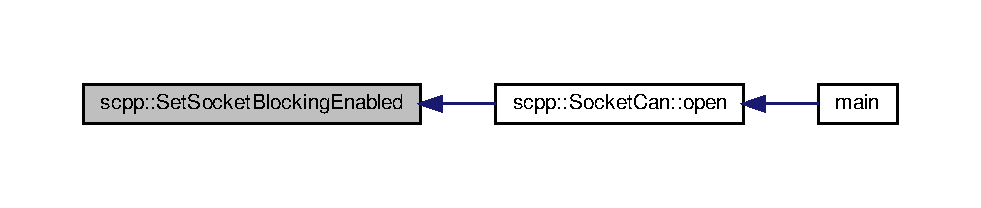
\includegraphics[width=350pt]{namespacescpp_a7acc4f95274c9fdd3fccecbb5e0a9b4c_icgraph}
\end{center}
\end{figure}

\chapter{Class Documentation}
\hypertarget{classCanBuffer}{}\section{Can\+Buffer Class Reference}
\label{classCanBuffer}\index{Can\+Buffer@{Can\+Buffer}}


{\ttfamily \#include $<$can\+\_\+buffer.\+h$>$}



Collaboration diagram for Can\+Buffer\+:
\nopagebreak
\begin{figure}[H]
\begin{center}
\leavevmode
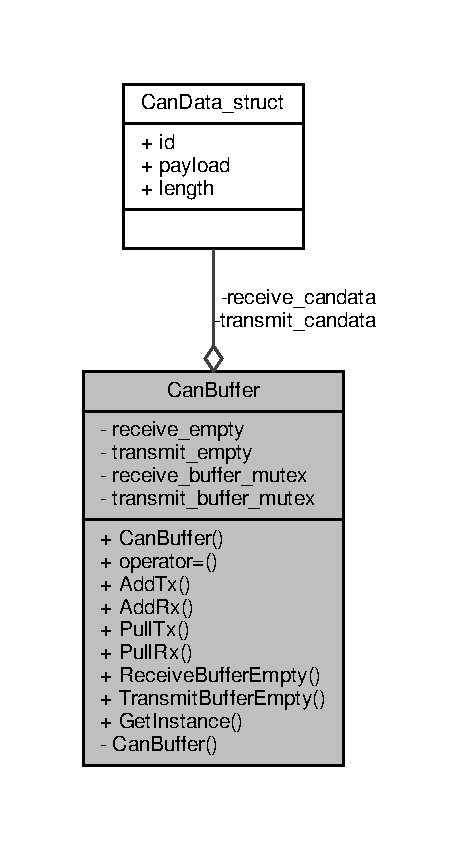
\includegraphics[width=222pt]{classCanBuffer__coll__graph}
\end{center}
\end{figure}
\subsection*{Public Member Functions}
\begin{DoxyCompactItemize}
\item 
\hyperlink{classCanBuffer_a02b0f8e006051bf73a8a0a70d0e919ec}{Can\+Buffer} (\hyperlink{classCanBuffer}{Can\+Buffer} const \&)=delete
\item 
void \hyperlink{classCanBuffer_aa2a1c35e5a3cf6106d78f986de53911d}{operator=} (\hyperlink{classCanBuffer}{Can\+Buffer} const \&)=delete
\item 
void \hyperlink{classCanBuffer_a9f61d33ebf8b9b98fb30998074351b90}{Add\+Tx} (const uint32\+\_\+t $\ast$id, uint8\+\_\+t payload\mbox{[}$\,$\mbox{]}, const uint8\+\_\+t $\ast$length)
\item 
void \hyperlink{classCanBuffer_a2038c19fd2b63223a86a48a8faef2996}{Add\+Rx} (const uint32\+\_\+t $\ast$id, uint8\+\_\+t payload\mbox{[}$\,$\mbox{]}, const uint8\+\_\+t $\ast$length)
\item 
\hyperlink{can__buffer_8h_a7a5dfa274d7d04c73e0b6b3e4dbbb87c}{Can\+Data} \hyperlink{classCanBuffer_a06cbabdf2a97378a2d4cd9120e909d53}{Pull\+Tx} ()
\item 
\hyperlink{can__buffer_8h_a7a5dfa274d7d04c73e0b6b3e4dbbb87c}{Can\+Data} \hyperlink{classCanBuffer_a66691d3306e47774f768fd391fff1802}{Pull\+Rx} ()
\item 
bool \hyperlink{classCanBuffer_a4b9e4e25a3312729bc64b0a7e7e80abf}{Receive\+Buffer\+Empty} ()
\item 
bool \hyperlink{classCanBuffer_a3826a986a95c4eb24f363a7ace01bec2}{Transmit\+Buffer\+Empty} ()
\end{DoxyCompactItemize}
\subsection*{Static Public Member Functions}
\begin{DoxyCompactItemize}
\item 
static \hyperlink{classCanBuffer}{Can\+Buffer} \& \hyperlink{classCanBuffer_add61873bc4e32e5b79ca665c1926f3b9}{Get\+Instance} ()
\end{DoxyCompactItemize}
\subsection*{Private Member Functions}
\begin{DoxyCompactItemize}
\item 
\hyperlink{classCanBuffer_a48282381b606242cfc4163e445c85409}{Can\+Buffer} ()
\end{DoxyCompactItemize}
\subsection*{Private Attributes}
\begin{DoxyCompactItemize}
\item 
\hyperlink{can__buffer_8h_a7a5dfa274d7d04c73e0b6b3e4dbbb87c}{Can\+Data} \hyperlink{classCanBuffer_a2f9526d98638e5c92695ba208a1a6084}{receive\+\_\+candata}
\item 
\hyperlink{can__buffer_8h_a7a5dfa274d7d04c73e0b6b3e4dbbb87c}{Can\+Data} \hyperlink{classCanBuffer_a8b7056beaeb5970d637001adb4722302}{transmit\+\_\+candata}
\item 
bool \hyperlink{classCanBuffer_a7a06170000a5bb8e66d6feed7ade64ad}{receive\+\_\+empty} = true
\item 
bool \hyperlink{classCanBuffer_a60d0c06e2b6ec133bc3d2b99872dc536}{transmit\+\_\+empty} = true
\item 
std\+::mutex \hyperlink{classCanBuffer_a99e2db7eb22a8f25ca92d5c5e791e99f}{receive\+\_\+buffer\+\_\+mutex}
\item 
std\+::mutex \hyperlink{classCanBuffer_aea5dc877a2bcdec8d3da11649346ca21}{transmit\+\_\+buffer\+\_\+mutex}
\end{DoxyCompactItemize}


\subsection{Constructor \& Destructor Documentation}
\mbox{\Hypertarget{classCanBuffer_a02b0f8e006051bf73a8a0a70d0e919ec}\label{classCanBuffer_a02b0f8e006051bf73a8a0a70d0e919ec}} 
\index{Can\+Buffer@{Can\+Buffer}!Can\+Buffer@{Can\+Buffer}}
\index{Can\+Buffer@{Can\+Buffer}!Can\+Buffer@{Can\+Buffer}}
\subsubsection{\texorpdfstring{Can\+Buffer()}{CanBuffer()}\hspace{0.1cm}{\footnotesize\ttfamily [1/2]}}
{\footnotesize\ttfamily Can\+Buffer\+::\+Can\+Buffer (\begin{DoxyParamCaption}\item[{\hyperlink{classCanBuffer}{Can\+Buffer} const \&}]{ }\end{DoxyParamCaption})\hspace{0.3cm}{\ttfamily [delete]}}

\mbox{\Hypertarget{classCanBuffer_a48282381b606242cfc4163e445c85409}\label{classCanBuffer_a48282381b606242cfc4163e445c85409}} 
\index{Can\+Buffer@{Can\+Buffer}!Can\+Buffer@{Can\+Buffer}}
\index{Can\+Buffer@{Can\+Buffer}!Can\+Buffer@{Can\+Buffer}}
\subsubsection{\texorpdfstring{Can\+Buffer()}{CanBuffer()}\hspace{0.1cm}{\footnotesize\ttfamily [2/2]}}
{\footnotesize\ttfamily Can\+Buffer\+::\+Can\+Buffer (\begin{DoxyParamCaption}{ }\end{DoxyParamCaption})\hspace{0.3cm}{\ttfamily [inline]}, {\ttfamily [private]}}



\subsection{Member Function Documentation}
\mbox{\Hypertarget{classCanBuffer_a2038c19fd2b63223a86a48a8faef2996}\label{classCanBuffer_a2038c19fd2b63223a86a48a8faef2996}} 
\index{Can\+Buffer@{Can\+Buffer}!Add\+Rx@{Add\+Rx}}
\index{Add\+Rx@{Add\+Rx}!Can\+Buffer@{Can\+Buffer}}
\subsubsection{\texorpdfstring{Add\+Rx()}{AddRx()}}
{\footnotesize\ttfamily void Can\+Buffer\+::\+Add\+Rx (\begin{DoxyParamCaption}\item[{const uint32\+\_\+t $\ast$}]{id,  }\item[{uint8\+\_\+t}]{payload\mbox{[}$\,$\mbox{]},  }\item[{const uint8\+\_\+t $\ast$}]{length }\end{DoxyParamCaption})}


\begin{DoxyItemize}
\item Adds received can data to the receive (RX) buffer 
\begin{DoxyParams}{Parameters}
{\em data} & received can data \\
\hline
\end{DoxyParams}

\end{DoxyItemize}Here is the caller graph for this function\+:
\nopagebreak
\begin{figure}[H]
\begin{center}
\leavevmode
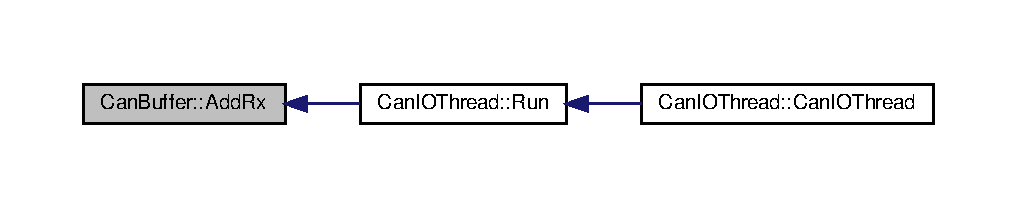
\includegraphics[width=350pt]{classCanBuffer_a2038c19fd2b63223a86a48a8faef2996_icgraph}
\end{center}
\end{figure}
\mbox{\Hypertarget{classCanBuffer_a9f61d33ebf8b9b98fb30998074351b90}\label{classCanBuffer_a9f61d33ebf8b9b98fb30998074351b90}} 
\index{Can\+Buffer@{Can\+Buffer}!Add\+Tx@{Add\+Tx}}
\index{Add\+Tx@{Add\+Tx}!Can\+Buffer@{Can\+Buffer}}
\subsubsection{\texorpdfstring{Add\+Tx()}{AddTx()}}
{\footnotesize\ttfamily void Can\+Buffer\+::\+Add\+Tx (\begin{DoxyParamCaption}\item[{const uint32\+\_\+t $\ast$}]{id,  }\item[{uint8\+\_\+t}]{payload\mbox{[}$\,$\mbox{]},  }\item[{const uint8\+\_\+t $\ast$}]{length }\end{DoxyParamCaption})}

Adds data to be sent to the transmit (TX) buffer 
\begin{DoxyParams}{Parameters}
{\em data} & data to be transmitted \\
\hline
\end{DoxyParams}
Here is the caller graph for this function\+:
\nopagebreak
\begin{figure}[H]
\begin{center}
\leavevmode
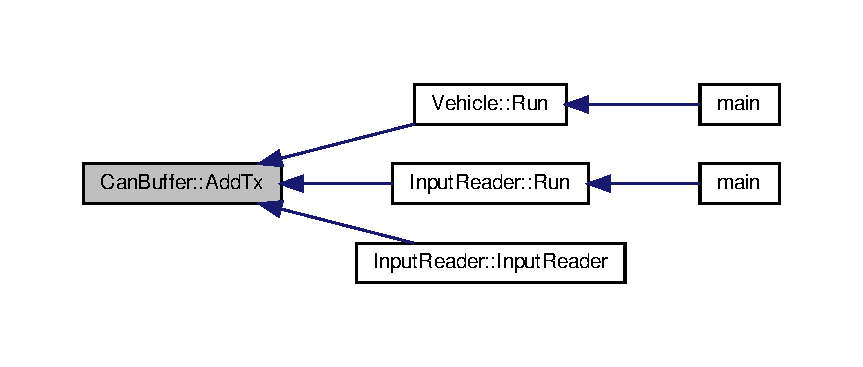
\includegraphics[width=350pt]{classCanBuffer_a9f61d33ebf8b9b98fb30998074351b90_icgraph}
\end{center}
\end{figure}
\mbox{\Hypertarget{classCanBuffer_add61873bc4e32e5b79ca665c1926f3b9}\label{classCanBuffer_add61873bc4e32e5b79ca665c1926f3b9}} 
\index{Can\+Buffer@{Can\+Buffer}!Get\+Instance@{Get\+Instance}}
\index{Get\+Instance@{Get\+Instance}!Can\+Buffer@{Can\+Buffer}}
\subsubsection{\texorpdfstring{Get\+Instance()}{GetInstance()}}
{\footnotesize\ttfamily static \hyperlink{classCanBuffer}{Can\+Buffer}\& Can\+Buffer\+::\+Get\+Instance (\begin{DoxyParamCaption}{ }\end{DoxyParamCaption})\hspace{0.3cm}{\ttfamily [inline]}, {\ttfamily [static]}}

Here is the caller graph for this function\+:
\nopagebreak
\begin{figure}[H]
\begin{center}
\leavevmode
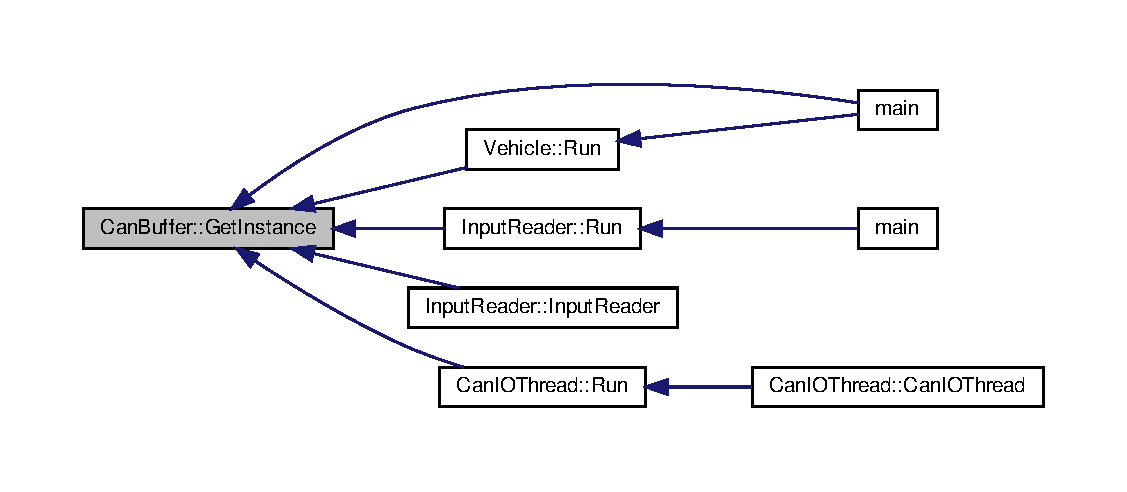
\includegraphics[width=350pt]{classCanBuffer_add61873bc4e32e5b79ca665c1926f3b9_icgraph}
\end{center}
\end{figure}
\mbox{\Hypertarget{classCanBuffer_aa2a1c35e5a3cf6106d78f986de53911d}\label{classCanBuffer_aa2a1c35e5a3cf6106d78f986de53911d}} 
\index{Can\+Buffer@{Can\+Buffer}!operator=@{operator=}}
\index{operator=@{operator=}!Can\+Buffer@{Can\+Buffer}}
\subsubsection{\texorpdfstring{operator=()}{operator=()}}
{\footnotesize\ttfamily void Can\+Buffer\+::operator= (\begin{DoxyParamCaption}\item[{\hyperlink{classCanBuffer}{Can\+Buffer} const \&}]{ }\end{DoxyParamCaption})\hspace{0.3cm}{\ttfamily [delete]}}

\mbox{\Hypertarget{classCanBuffer_a66691d3306e47774f768fd391fff1802}\label{classCanBuffer_a66691d3306e47774f768fd391fff1802}} 
\index{Can\+Buffer@{Can\+Buffer}!Pull\+Rx@{Pull\+Rx}}
\index{Pull\+Rx@{Pull\+Rx}!Can\+Buffer@{Can\+Buffer}}
\subsubsection{\texorpdfstring{Pull\+Rx()}{PullRx()}}
{\footnotesize\ttfamily \hyperlink{can__buffer_8h_a7a5dfa274d7d04c73e0b6b3e4dbbb87c}{Can\+Data} Can\+Buffer\+::\+Pull\+Rx (\begin{DoxyParamCaption}{ }\end{DoxyParamCaption})}

Pulls next data package from the receive (RX) buffer \begin{DoxyReturn}{Returns}
received data 
\end{DoxyReturn}
Here is the caller graph for this function\+:
\nopagebreak
\begin{figure}[H]
\begin{center}
\leavevmode
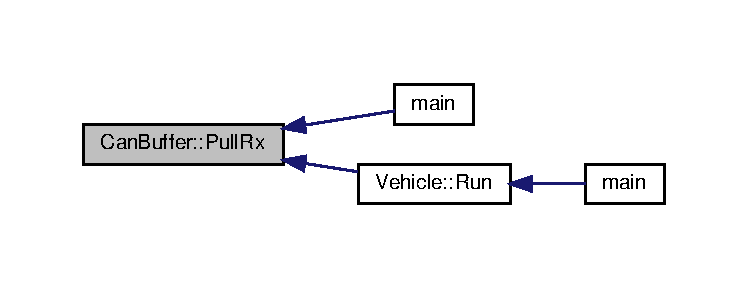
\includegraphics[width=350pt]{classCanBuffer_a66691d3306e47774f768fd391fff1802_icgraph}
\end{center}
\end{figure}
\mbox{\Hypertarget{classCanBuffer_a06cbabdf2a97378a2d4cd9120e909d53}\label{classCanBuffer_a06cbabdf2a97378a2d4cd9120e909d53}} 
\index{Can\+Buffer@{Can\+Buffer}!Pull\+Tx@{Pull\+Tx}}
\index{Pull\+Tx@{Pull\+Tx}!Can\+Buffer@{Can\+Buffer}}
\subsubsection{\texorpdfstring{Pull\+Tx()}{PullTx()}}
{\footnotesize\ttfamily \hyperlink{can__buffer_8h_a7a5dfa274d7d04c73e0b6b3e4dbbb87c}{Can\+Data} Can\+Buffer\+::\+Pull\+Tx (\begin{DoxyParamCaption}{ }\end{DoxyParamCaption})}

Pulls next data package from the transmit (TX) buffer \begin{DoxyReturn}{Returns}
data to be transmitted 
\end{DoxyReturn}
Here is the caller graph for this function\+:
\nopagebreak
\begin{figure}[H]
\begin{center}
\leavevmode
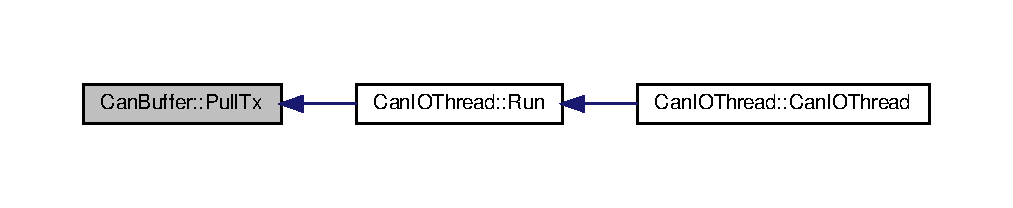
\includegraphics[width=350pt]{classCanBuffer_a06cbabdf2a97378a2d4cd9120e909d53_icgraph}
\end{center}
\end{figure}
\mbox{\Hypertarget{classCanBuffer_a4b9e4e25a3312729bc64b0a7e7e80abf}\label{classCanBuffer_a4b9e4e25a3312729bc64b0a7e7e80abf}} 
\index{Can\+Buffer@{Can\+Buffer}!Receive\+Buffer\+Empty@{Receive\+Buffer\+Empty}}
\index{Receive\+Buffer\+Empty@{Receive\+Buffer\+Empty}!Can\+Buffer@{Can\+Buffer}}
\subsubsection{\texorpdfstring{Receive\+Buffer\+Empty()}{ReceiveBufferEmpty()}}
{\footnotesize\ttfamily bool Can\+Buffer\+::\+Receive\+Buffer\+Empty (\begin{DoxyParamCaption}{ }\end{DoxyParamCaption})}

Check if receive buffer contains any elements \begin{DoxyReturn}{Returns}
T\+R\+UE if receive buffer is empty 
\end{DoxyReturn}
\mbox{\Hypertarget{classCanBuffer_a3826a986a95c4eb24f363a7ace01bec2}\label{classCanBuffer_a3826a986a95c4eb24f363a7ace01bec2}} 
\index{Can\+Buffer@{Can\+Buffer}!Transmit\+Buffer\+Empty@{Transmit\+Buffer\+Empty}}
\index{Transmit\+Buffer\+Empty@{Transmit\+Buffer\+Empty}!Can\+Buffer@{Can\+Buffer}}
\subsubsection{\texorpdfstring{Transmit\+Buffer\+Empty()}{TransmitBufferEmpty()}}
{\footnotesize\ttfamily bool Can\+Buffer\+::\+Transmit\+Buffer\+Empty (\begin{DoxyParamCaption}{ }\end{DoxyParamCaption})}

Check if transmit buffer contains any elements \begin{DoxyReturn}{Returns}
T\+R\+UE if transmit buffer is empty 
\end{DoxyReturn}


\subsection{Member Data Documentation}
\mbox{\Hypertarget{classCanBuffer_a99e2db7eb22a8f25ca92d5c5e791e99f}\label{classCanBuffer_a99e2db7eb22a8f25ca92d5c5e791e99f}} 
\index{Can\+Buffer@{Can\+Buffer}!receive\+\_\+buffer\+\_\+mutex@{receive\+\_\+buffer\+\_\+mutex}}
\index{receive\+\_\+buffer\+\_\+mutex@{receive\+\_\+buffer\+\_\+mutex}!Can\+Buffer@{Can\+Buffer}}
\subsubsection{\texorpdfstring{receive\+\_\+buffer\+\_\+mutex}{receive\_buffer\_mutex}}
{\footnotesize\ttfamily std\+::mutex Can\+Buffer\+::receive\+\_\+buffer\+\_\+mutex\hspace{0.3cm}{\ttfamily [private]}}

\mbox{\Hypertarget{classCanBuffer_a2f9526d98638e5c92695ba208a1a6084}\label{classCanBuffer_a2f9526d98638e5c92695ba208a1a6084}} 
\index{Can\+Buffer@{Can\+Buffer}!receive\+\_\+candata@{receive\+\_\+candata}}
\index{receive\+\_\+candata@{receive\+\_\+candata}!Can\+Buffer@{Can\+Buffer}}
\subsubsection{\texorpdfstring{receive\+\_\+candata}{receive\_candata}}
{\footnotesize\ttfamily \hyperlink{can__buffer_8h_a7a5dfa274d7d04c73e0b6b3e4dbbb87c}{Can\+Data} Can\+Buffer\+::receive\+\_\+candata\hspace{0.3cm}{\ttfamily [private]}}

\mbox{\Hypertarget{classCanBuffer_a7a06170000a5bb8e66d6feed7ade64ad}\label{classCanBuffer_a7a06170000a5bb8e66d6feed7ade64ad}} 
\index{Can\+Buffer@{Can\+Buffer}!receive\+\_\+empty@{receive\+\_\+empty}}
\index{receive\+\_\+empty@{receive\+\_\+empty}!Can\+Buffer@{Can\+Buffer}}
\subsubsection{\texorpdfstring{receive\+\_\+empty}{receive\_empty}}
{\footnotesize\ttfamily bool Can\+Buffer\+::receive\+\_\+empty = true\hspace{0.3cm}{\ttfamily [private]}}

\mbox{\Hypertarget{classCanBuffer_aea5dc877a2bcdec8d3da11649346ca21}\label{classCanBuffer_aea5dc877a2bcdec8d3da11649346ca21}} 
\index{Can\+Buffer@{Can\+Buffer}!transmit\+\_\+buffer\+\_\+mutex@{transmit\+\_\+buffer\+\_\+mutex}}
\index{transmit\+\_\+buffer\+\_\+mutex@{transmit\+\_\+buffer\+\_\+mutex}!Can\+Buffer@{Can\+Buffer}}
\subsubsection{\texorpdfstring{transmit\+\_\+buffer\+\_\+mutex}{transmit\_buffer\_mutex}}
{\footnotesize\ttfamily std\+::mutex Can\+Buffer\+::transmit\+\_\+buffer\+\_\+mutex\hspace{0.3cm}{\ttfamily [private]}}

\mbox{\Hypertarget{classCanBuffer_a8b7056beaeb5970d637001adb4722302}\label{classCanBuffer_a8b7056beaeb5970d637001adb4722302}} 
\index{Can\+Buffer@{Can\+Buffer}!transmit\+\_\+candata@{transmit\+\_\+candata}}
\index{transmit\+\_\+candata@{transmit\+\_\+candata}!Can\+Buffer@{Can\+Buffer}}
\subsubsection{\texorpdfstring{transmit\+\_\+candata}{transmit\_candata}}
{\footnotesize\ttfamily \hyperlink{can__buffer_8h_a7a5dfa274d7d04c73e0b6b3e4dbbb87c}{Can\+Data} Can\+Buffer\+::transmit\+\_\+candata\hspace{0.3cm}{\ttfamily [private]}}

\mbox{\Hypertarget{classCanBuffer_a60d0c06e2b6ec133bc3d2b99872dc536}\label{classCanBuffer_a60d0c06e2b6ec133bc3d2b99872dc536}} 
\index{Can\+Buffer@{Can\+Buffer}!transmit\+\_\+empty@{transmit\+\_\+empty}}
\index{transmit\+\_\+empty@{transmit\+\_\+empty}!Can\+Buffer@{Can\+Buffer}}
\subsubsection{\texorpdfstring{transmit\+\_\+empty}{transmit\_empty}}
{\footnotesize\ttfamily bool Can\+Buffer\+::transmit\+\_\+empty = true\hspace{0.3cm}{\ttfamily [private]}}



The documentation for this class was generated from the following files\+:\begin{DoxyCompactItemize}
\item 
/home/rjohan59/repos/bootcamp\+\_\+course/project/source\+\_\+code/utils/include/\hyperlink{can__buffer_8h}{can\+\_\+buffer.\+h}\item 
/home/rjohan59/repos/bootcamp\+\_\+course/project/source\+\_\+code/utils/src/\hyperlink{can__buffer_8cpp}{can\+\_\+buffer.\+cpp}\end{DoxyCompactItemize}

\hypertarget{structCanData__struct}{}\section{Can\+Data\+\_\+struct Struct Reference}
\label{structCanData__struct}\index{Can\+Data\+\_\+struct@{Can\+Data\+\_\+struct}}


{\ttfamily \#include $<$can\+\_\+buffer.\+h$>$}



Collaboration diagram for Can\+Data\+\_\+struct\+:
\nopagebreak
\begin{figure}[H]
\begin{center}
\leavevmode
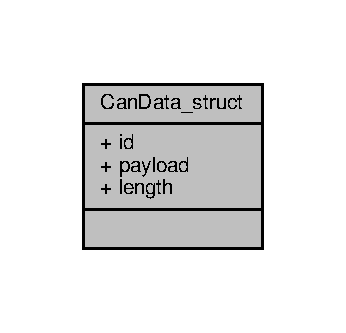
\includegraphics[width=166pt]{structCanData__struct__coll__graph}
\end{center}
\end{figure}
\subsection*{Public Attributes}
\begin{DoxyCompactItemize}
\item 
uint32\+\_\+t \hyperlink{structCanData__struct_a1f6f5483251189fc5819762739e6e84d}{id} = 0
\item 
uint8\+\_\+t \hyperlink{structCanData__struct_a0da7d3f1624043fc775968620c0be651}{payload} \mbox{[}8\mbox{]} = \{0,0,0,0,0,0,0,0\}
\item 
uint8\+\_\+t \hyperlink{structCanData__struct_ad1ca4194a316ab04be6e24276fb20055}{length} = 0
\end{DoxyCompactItemize}


\subsection{Member Data Documentation}
\mbox{\Hypertarget{structCanData__struct_a1f6f5483251189fc5819762739e6e84d}\label{structCanData__struct_a1f6f5483251189fc5819762739e6e84d}} 
\index{Can\+Data\+\_\+struct@{Can\+Data\+\_\+struct}!id@{id}}
\index{id@{id}!Can\+Data\+\_\+struct@{Can\+Data\+\_\+struct}}
\subsubsection{\texorpdfstring{id}{id}}
{\footnotesize\ttfamily uint32\+\_\+t Can\+Data\+\_\+struct\+::id = 0}

\mbox{\Hypertarget{structCanData__struct_ad1ca4194a316ab04be6e24276fb20055}\label{structCanData__struct_ad1ca4194a316ab04be6e24276fb20055}} 
\index{Can\+Data\+\_\+struct@{Can\+Data\+\_\+struct}!length@{length}}
\index{length@{length}!Can\+Data\+\_\+struct@{Can\+Data\+\_\+struct}}
\subsubsection{\texorpdfstring{length}{length}}
{\footnotesize\ttfamily uint8\+\_\+t Can\+Data\+\_\+struct\+::length = 0}

\mbox{\Hypertarget{structCanData__struct_a0da7d3f1624043fc775968620c0be651}\label{structCanData__struct_a0da7d3f1624043fc775968620c0be651}} 
\index{Can\+Data\+\_\+struct@{Can\+Data\+\_\+struct}!payload@{payload}}
\index{payload@{payload}!Can\+Data\+\_\+struct@{Can\+Data\+\_\+struct}}
\subsubsection{\texorpdfstring{payload}{payload}}
{\footnotesize\ttfamily uint8\+\_\+t Can\+Data\+\_\+struct\+::payload\mbox{[}8\mbox{]} = \{0,0,0,0,0,0,0,0\}}



The documentation for this struct was generated from the following file\+:\begin{DoxyCompactItemize}
\item 
/home/rjohan59/repos/bootcamp\+\_\+course/project/source\+\_\+code/utils/include/\hyperlink{can__buffer_8h}{can\+\_\+buffer.\+h}\end{DoxyCompactItemize}

\hypertarget{structscpp_1_1CanFrame}{}\section{scpp\+:\+:Can\+Frame Struct Reference}
\label{structscpp_1_1CanFrame}\index{scpp\+::\+Can\+Frame@{scpp\+::\+Can\+Frame}}


{\ttfamily \#include $<$socketcan.\+h$>$}



Collaboration diagram for scpp\+:\+:Can\+Frame\+:
\nopagebreak
\begin{figure}[H]
\begin{center}
\leavevmode
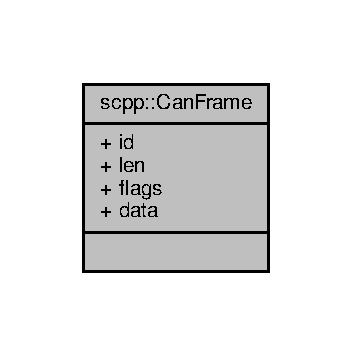
\includegraphics[width=169pt]{structscpp_1_1CanFrame__coll__graph}
\end{center}
\end{figure}
\subsection*{Public Attributes}
\begin{DoxyCompactItemize}
\item 
uint32\+\_\+t \hyperlink{structscpp_1_1CanFrame_a926c47e6fa4f8a2809b31ac85cc89b15}{id} = 0
\item 
uint8\+\_\+t \hyperlink{structscpp_1_1CanFrame_ab949305fcfb1820ea8ca338bfad7fe6a}{len} = 0
\item 
uint8\+\_\+t \hyperlink{structscpp_1_1CanFrame_a4b548ba3048832804bca2c05d6ee4787}{flags} = 0
\item 
uint8\+\_\+t \hyperlink{structscpp_1_1CanFrame_a61f2cb4a342280cd8710c22c3d672db5}{data} \mbox{[}64\mbox{]}
\end{DoxyCompactItemize}


\subsection{Member Data Documentation}
\mbox{\Hypertarget{structscpp_1_1CanFrame_a61f2cb4a342280cd8710c22c3d672db5}\label{structscpp_1_1CanFrame_a61f2cb4a342280cd8710c22c3d672db5}} 
\index{scpp\+::\+Can\+Frame@{scpp\+::\+Can\+Frame}!data@{data}}
\index{data@{data}!scpp\+::\+Can\+Frame@{scpp\+::\+Can\+Frame}}
\subsubsection{\texorpdfstring{data}{data}}
{\footnotesize\ttfamily uint8\+\_\+t scpp\+::\+Can\+Frame\+::data\mbox{[}64\mbox{]}}

\mbox{\Hypertarget{structscpp_1_1CanFrame_a4b548ba3048832804bca2c05d6ee4787}\label{structscpp_1_1CanFrame_a4b548ba3048832804bca2c05d6ee4787}} 
\index{scpp\+::\+Can\+Frame@{scpp\+::\+Can\+Frame}!flags@{flags}}
\index{flags@{flags}!scpp\+::\+Can\+Frame@{scpp\+::\+Can\+Frame}}
\subsubsection{\texorpdfstring{flags}{flags}}
{\footnotesize\ttfamily uint8\+\_\+t scpp\+::\+Can\+Frame\+::flags = 0}

\mbox{\Hypertarget{structscpp_1_1CanFrame_a926c47e6fa4f8a2809b31ac85cc89b15}\label{structscpp_1_1CanFrame_a926c47e6fa4f8a2809b31ac85cc89b15}} 
\index{scpp\+::\+Can\+Frame@{scpp\+::\+Can\+Frame}!id@{id}}
\index{id@{id}!scpp\+::\+Can\+Frame@{scpp\+::\+Can\+Frame}}
\subsubsection{\texorpdfstring{id}{id}}
{\footnotesize\ttfamily uint32\+\_\+t scpp\+::\+Can\+Frame\+::id = 0}

\mbox{\Hypertarget{structscpp_1_1CanFrame_ab949305fcfb1820ea8ca338bfad7fe6a}\label{structscpp_1_1CanFrame_ab949305fcfb1820ea8ca338bfad7fe6a}} 
\index{scpp\+::\+Can\+Frame@{scpp\+::\+Can\+Frame}!len@{len}}
\index{len@{len}!scpp\+::\+Can\+Frame@{scpp\+::\+Can\+Frame}}
\subsubsection{\texorpdfstring{len}{len}}
{\footnotesize\ttfamily uint8\+\_\+t scpp\+::\+Can\+Frame\+::len = 0}



The documentation for this struct was generated from the following file\+:\begin{DoxyCompactItemize}
\item 
/home/rjohan59/repos/bootcamp\+\_\+course/project/source\+\_\+code/utils/include/\hyperlink{socketcan_8h}{socketcan.\+h}\end{DoxyCompactItemize}

\hypertarget{classCanIOThread}{}\section{Can\+I\+O\+Thread Class Reference}
\label{classCanIOThread}\index{Can\+I\+O\+Thread@{Can\+I\+O\+Thread}}


{\ttfamily \#include $<$can\+\_\+io\+\_\+thread.\+h$>$}



Collaboration diagram for Can\+I\+O\+Thread\+:
\nopagebreak
\begin{figure}[H]
\begin{center}
\leavevmode
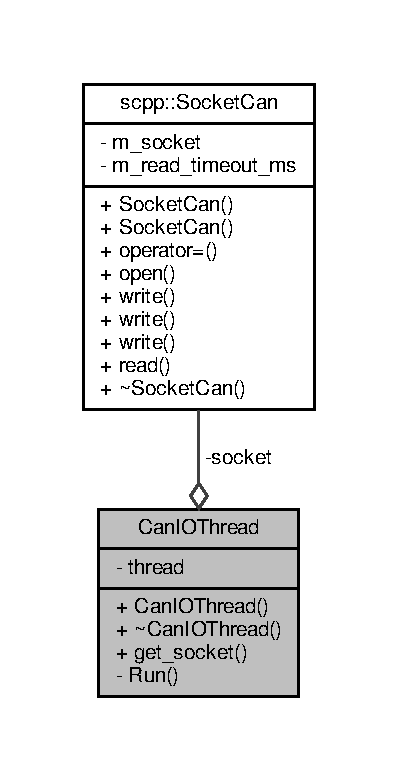
\includegraphics[width=191pt]{classCanIOThread__coll__graph}
\end{center}
\end{figure}
\subsection*{Public Member Functions}
\begin{DoxyCompactItemize}
\item 
\hyperlink{classCanIOThread_a5ab76331e5bd6ce26fcad85e8bd5d9f4}{Can\+I\+O\+Thread} (\hyperlink{classscpp_1_1SocketCan}{scpp\+::\+Socket\+Can} $\ast$\hyperlink{classCanIOThread_a4c0f06e7c73ea3afcb567ff7dbb41f30}{socket}, std\+::future$<$ void $>$ $\ast$future, uint8\+\_\+t $\ast$receive\+\_\+message\+\_\+id, const size\+\_\+t \&receive\+\_\+message\+\_\+id\+\_\+size)
\item 
\hyperlink{classCanIOThread_acbe9fb01fc351b5d0babe204ff086e5b}{$\sim$\+Can\+I\+O\+Thread} ()
\item 
\hyperlink{classscpp_1_1SocketCan}{scpp\+::\+Socket\+Can} $\ast$ \hyperlink{classCanIOThread_abd81d2bfe629d2abf8a3ee4e0d71c7e5}{get\+\_\+socket} ()
\end{DoxyCompactItemize}
\subsection*{Private Member Functions}
\begin{DoxyCompactItemize}
\item 
void \hyperlink{classCanIOThread_a1dfe981584e3e558df59211571ac9860}{Run} (std\+::future$<$ void $>$ $\ast$future, uint8\+\_\+t $\ast$receive\+\_\+message\+\_\+id, const size\+\_\+t \&receive\+\_\+message\+\_\+id\+\_\+size)
\end{DoxyCompactItemize}
\subsection*{Private Attributes}
\begin{DoxyCompactItemize}
\item 
std\+::thread \hyperlink{classCanIOThread_a7a0b5ee8f944e3e94d529311f064c1ac}{thread}
\item 
\hyperlink{classscpp_1_1SocketCan}{scpp\+::\+Socket\+Can} $\ast$ \hyperlink{classCanIOThread_a4c0f06e7c73ea3afcb567ff7dbb41f30}{socket}
\end{DoxyCompactItemize}


\subsection{Constructor \& Destructor Documentation}
\mbox{\Hypertarget{classCanIOThread_a5ab76331e5bd6ce26fcad85e8bd5d9f4}\label{classCanIOThread_a5ab76331e5bd6ce26fcad85e8bd5d9f4}} 
\index{Can\+I\+O\+Thread@{Can\+I\+O\+Thread}!Can\+I\+O\+Thread@{Can\+I\+O\+Thread}}
\index{Can\+I\+O\+Thread@{Can\+I\+O\+Thread}!Can\+I\+O\+Thread@{Can\+I\+O\+Thread}}
\subsubsection{\texorpdfstring{Can\+I\+O\+Thread()}{CanIOThread()}}
{\footnotesize\ttfamily Can\+I\+O\+Thread\+::\+Can\+I\+O\+Thread (\begin{DoxyParamCaption}\item[{\hyperlink{classscpp_1_1SocketCan}{scpp\+::\+Socket\+Can} $\ast$}]{socket,  }\item[{std\+::future$<$ void $>$ $\ast$}]{future,  }\item[{uint8\+\_\+t $\ast$}]{receive\+\_\+message\+\_\+id,  }\item[{const size\+\_\+t \&}]{receive\+\_\+message\+\_\+id\+\_\+size }\end{DoxyParamCaption})}

Constructor of \hyperlink{classCanIOThread}{Can\+I\+O\+Thread}. Assigns the class members and starts a thread on the function \char`\"{}\+Run\char`\"{} 
\begin{DoxyParams}{Parameters}
{\em socket} & used for read and write data to can \\
\hline
{\em receive\+\_\+message\+\_\+id} & list of I\+Ds that should be read \\
\hline
{\em receive\+\_\+message\+\_\+id\+\_\+size} & size of the list receive\+\_\+message\+\_\+id. \\
\hline
\end{DoxyParams}
Here is the call graph for this function\+:
\nopagebreak
\begin{figure}[H]
\begin{center}
\leavevmode
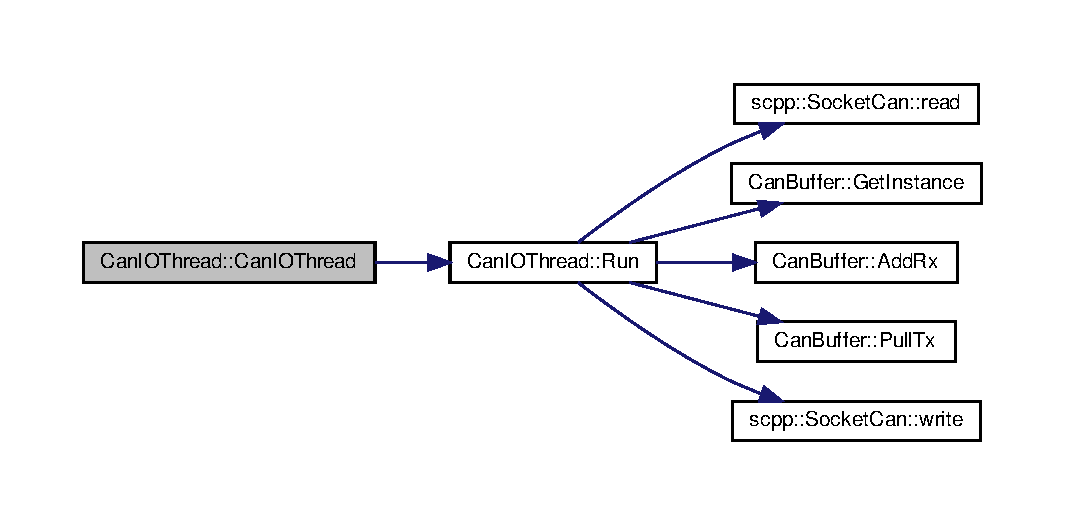
\includegraphics[width=350pt]{classCanIOThread_a5ab76331e5bd6ce26fcad85e8bd5d9f4_cgraph}
\end{center}
\end{figure}
\mbox{\Hypertarget{classCanIOThread_acbe9fb01fc351b5d0babe204ff086e5b}\label{classCanIOThread_acbe9fb01fc351b5d0babe204ff086e5b}} 
\index{Can\+I\+O\+Thread@{Can\+I\+O\+Thread}!````~Can\+I\+O\+Thread@{$\sim$\+Can\+I\+O\+Thread}}
\index{````~Can\+I\+O\+Thread@{$\sim$\+Can\+I\+O\+Thread}!Can\+I\+O\+Thread@{Can\+I\+O\+Thread}}
\subsubsection{\texorpdfstring{$\sim$\+Can\+I\+O\+Thread()}{~CanIOThread()}}
{\footnotesize\ttfamily Can\+I\+O\+Thread\+::$\sim$\+Can\+I\+O\+Thread (\begin{DoxyParamCaption}{ }\end{DoxyParamCaption})}

Destructor of \hyperlink{classCanIOThread}{Can\+I\+O\+Thread}. Informs the thread to stop (the Run function) and wait until it is done. 

\subsection{Member Function Documentation}
\mbox{\Hypertarget{classCanIOThread_abd81d2bfe629d2abf8a3ee4e0d71c7e5}\label{classCanIOThread_abd81d2bfe629d2abf8a3ee4e0d71c7e5}} 
\index{Can\+I\+O\+Thread@{Can\+I\+O\+Thread}!get\+\_\+socket@{get\+\_\+socket}}
\index{get\+\_\+socket@{get\+\_\+socket}!Can\+I\+O\+Thread@{Can\+I\+O\+Thread}}
\subsubsection{\texorpdfstring{get\+\_\+socket()}{get\_socket()}}
{\footnotesize\ttfamily \hyperlink{classscpp_1_1SocketCan}{scpp\+::\+Socket\+Can}$\ast$ Can\+I\+O\+Thread\+::get\+\_\+socket (\begin{DoxyParamCaption}{ }\end{DoxyParamCaption})}

\mbox{\Hypertarget{classCanIOThread_a1dfe981584e3e558df59211571ac9860}\label{classCanIOThread_a1dfe981584e3e558df59211571ac9860}} 
\index{Can\+I\+O\+Thread@{Can\+I\+O\+Thread}!Run@{Run}}
\index{Run@{Run}!Can\+I\+O\+Thread@{Can\+I\+O\+Thread}}
\subsubsection{\texorpdfstring{Run()}{Run()}}
{\footnotesize\ttfamily void Can\+I\+O\+Thread\+::\+Run (\begin{DoxyParamCaption}\item[{std\+::future$<$ void $>$ $\ast$}]{future,  }\item[{uint8\+\_\+t $\ast$}]{receive\+\_\+message\+\_\+id,  }\item[{const size\+\_\+t \&}]{receive\+\_\+message\+\_\+id\+\_\+size }\end{DoxyParamCaption})\hspace{0.3cm}{\ttfamily [private]}}

Reads data from C\+AN and writes it to the receive buffer. Pulls data from the transmit buffer and transmits it to can. Loops until a the future is set from outside of this class. 
\begin{DoxyParams}{Parameters}
{\em future} & future which will notify when the execution (the loop) should end \\
\hline
{\em receive\+\_\+message\+\_\+id} & list of I\+Ds that should be read \\
\hline
{\em receive\+\_\+message\+\_\+id\+\_\+size} & size of the list receive\+\_\+message\+\_\+id. \\
\hline
\end{DoxyParams}
Here is the call graph for this function\+:
\nopagebreak
\begin{figure}[H]
\begin{center}
\leavevmode
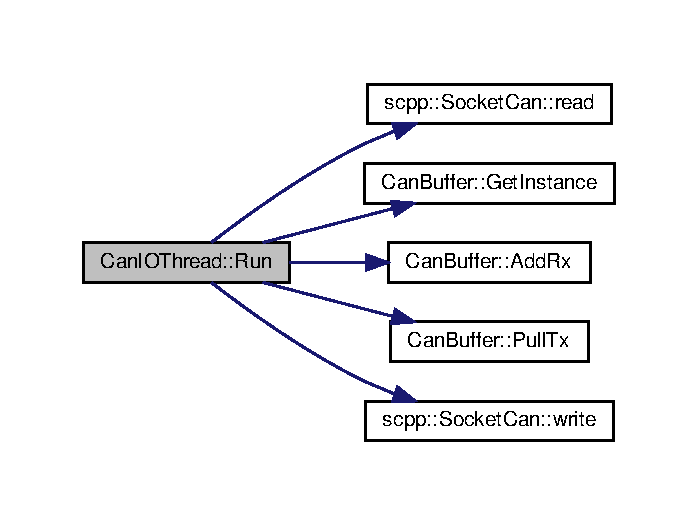
\includegraphics[width=335pt]{classCanIOThread_a1dfe981584e3e558df59211571ac9860_cgraph}
\end{center}
\end{figure}
Here is the caller graph for this function\+:
\nopagebreak
\begin{figure}[H]
\begin{center}
\leavevmode
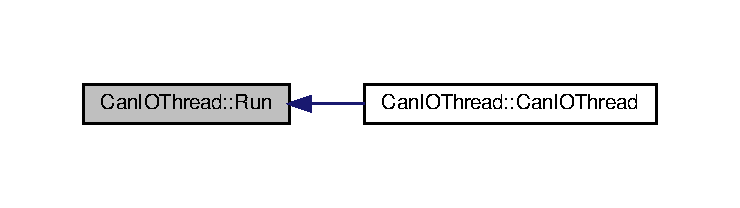
\includegraphics[width=350pt]{classCanIOThread_a1dfe981584e3e558df59211571ac9860_icgraph}
\end{center}
\end{figure}


\subsection{Member Data Documentation}
\mbox{\Hypertarget{classCanIOThread_a4c0f06e7c73ea3afcb567ff7dbb41f30}\label{classCanIOThread_a4c0f06e7c73ea3afcb567ff7dbb41f30}} 
\index{Can\+I\+O\+Thread@{Can\+I\+O\+Thread}!socket@{socket}}
\index{socket@{socket}!Can\+I\+O\+Thread@{Can\+I\+O\+Thread}}
\subsubsection{\texorpdfstring{socket}{socket}}
{\footnotesize\ttfamily \hyperlink{classscpp_1_1SocketCan}{scpp\+::\+Socket\+Can}$\ast$ Can\+I\+O\+Thread\+::socket\hspace{0.3cm}{\ttfamily [private]}}

\mbox{\Hypertarget{classCanIOThread_a7a0b5ee8f944e3e94d529311f064c1ac}\label{classCanIOThread_a7a0b5ee8f944e3e94d529311f064c1ac}} 
\index{Can\+I\+O\+Thread@{Can\+I\+O\+Thread}!thread@{thread}}
\index{thread@{thread}!Can\+I\+O\+Thread@{Can\+I\+O\+Thread}}
\subsubsection{\texorpdfstring{thread}{thread}}
{\footnotesize\ttfamily std\+::thread Can\+I\+O\+Thread\+::thread\hspace{0.3cm}{\ttfamily [private]}}



The documentation for this class was generated from the following files\+:\begin{DoxyCompactItemize}
\item 
/home/rjohan59/repos/bootcamp\+\_\+course/project/source\+\_\+code/utils/include/\hyperlink{can__io__thread_8h}{can\+\_\+io\+\_\+thread.\+h}\item 
/home/rjohan59/repos/bootcamp\+\_\+course/project/source\+\_\+code/utils/src/\hyperlink{can__io__thread_8cpp}{can\+\_\+io\+\_\+thread.\+cpp}\end{DoxyCompactItemize}

\hypertarget{classEngine}{}\section{Engine Class Reference}
\label{classEngine}\index{Engine@{Engine}}


{\ttfamily \#include $<$engine\+\_\+simulator.\+h$>$}



Collaboration diagram for Engine\+:
\nopagebreak
\begin{figure}[H]
\begin{center}
\leavevmode
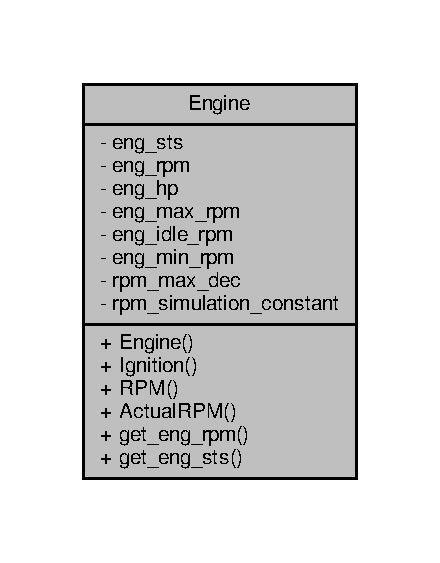
\includegraphics[width=211pt]{classEngine__coll__graph}
\end{center}
\end{figure}
\subsection*{Public Member Functions}
\begin{DoxyCompactItemize}
\item 
\hyperlink{classEngine_a756d6abb1d53627a0763f53490a774ef}{Engine} (const uint16\+\_\+t \&hp, const uint16\+\_\+t \&max\+\_\+rpm)
\item 
void \hyperlink{classEngine_a7e4b7cfcb9184beb80fed0ea60a3aad1}{Ignition} (const bool \&ign\+\_\+req, const uint8\+\_\+t \&speed, const uint8\+\_\+t \&brk\+\_\+pedal, const uint8\+\_\+t \&gear\+\_\+position)
\item 
void \hyperlink{classEngine_aaeaf10a957802225b43d088b5c2ce54b}{R\+PM} (const uint8\+\_\+t \&acc\+\_\+pedal, const uint8\+\_\+t \&brk\+\_\+pedal, const uint16\+\_\+t \&sampletime)
\item 
void \hyperlink{classEngine_a72bbd11160a8d916332b26e294133684}{Actual\+R\+PM} (const float \&speed, const float \&speed\+\_\+to\+\_\+rpm\+\_\+factor)
\item 
float \hyperlink{classEngine_a31646756334221f7967a114c64f188f4}{get\+\_\+eng\+\_\+rpm} ()
\item 
bool \hyperlink{classEngine_abf40022906338faef233d44a93ea01af}{get\+\_\+eng\+\_\+sts} ()
\end{DoxyCompactItemize}
\subsection*{Private Attributes}
\begin{DoxyCompactItemize}
\item 
bool \hyperlink{classEngine_a2c5cddbb86ed53703f2ed8182d505c82}{eng\+\_\+sts}
\item 
float \hyperlink{classEngine_aa502de3162f10d4e7f086cb08c817372}{eng\+\_\+rpm}
\item 
uint16\+\_\+t \hyperlink{classEngine_a450f51a16e7aa1af382193e8acf6e36a}{eng\+\_\+hp}
\item 
uint16\+\_\+t \hyperlink{classEngine_a2d840eecfbd0cc30d0063daee122b66f}{eng\+\_\+max\+\_\+rpm}
\item 
const uint16\+\_\+t \hyperlink{classEngine_a4a099af57c5bb8df6006aeab0e1f30ae}{eng\+\_\+idle\+\_\+rpm} = 900
\item 
const uint16\+\_\+t \hyperlink{classEngine_a83b157d748ed627fbeb06ae4a7b4514a}{eng\+\_\+min\+\_\+rpm} = 850
\item 
const uint16\+\_\+t \hyperlink{classEngine_ac03e3994b854b6ecbb3bf05dba2942a5}{rpm\+\_\+max\+\_\+dec} = 150
\item 
const float \hyperlink{classEngine_aac9426589cebccaa8cadf7cc7a0ba9be}{rpm\+\_\+simulation\+\_\+constant} = 5$\ast$pow(10,-\/7)
\end{DoxyCompactItemize}


\subsection{Constructor \& Destructor Documentation}
\mbox{\Hypertarget{classEngine_a756d6abb1d53627a0763f53490a774ef}\label{classEngine_a756d6abb1d53627a0763f53490a774ef}} 
\index{Engine@{Engine}!Engine@{Engine}}
\index{Engine@{Engine}!Engine@{Engine}}
\subsubsection{\texorpdfstring{Engine()}{Engine()}}
{\footnotesize\ttfamily Engine\+::\+Engine (\begin{DoxyParamCaption}\item[{const uint16\+\_\+t \&}]{hp,  }\item[{const uint16\+\_\+t \&}]{max\+\_\+rpm }\end{DoxyParamCaption})}

Constructor for \hyperlink{classEngine}{Engine}, sets horsepower and max rpm. 
\begin{DoxyParams}{Parameters}
{\em hp} & horsepower. \\
\hline
{\em max\+\_\+rpm} & maximum R\+PM. \\
\hline
\end{DoxyParams}


\subsection{Member Function Documentation}
\mbox{\Hypertarget{classEngine_a72bbd11160a8d916332b26e294133684}\label{classEngine_a72bbd11160a8d916332b26e294133684}} 
\index{Engine@{Engine}!Actual\+R\+PM@{Actual\+R\+PM}}
\index{Actual\+R\+PM@{Actual\+R\+PM}!Engine@{Engine}}
\subsubsection{\texorpdfstring{Actual\+R\+P\+M()}{ActualRPM()}}
{\footnotesize\ttfamily void Engine\+::\+Actual\+R\+PM (\begin{DoxyParamCaption}\item[{const float \&}]{speed,  }\item[{const float \&}]{speed\+\_\+to\+\_\+rpm\+\_\+factor }\end{DoxyParamCaption})}

Calculates actual R\+PM based on speed and speed to rpm factor. 
\begin{DoxyParams}{Parameters}
{\em speed} & current vehicle speed. \\
\hline
{\em speed\+\_\+to\+\_\+rpm\+\_\+factor} & factor to multiply with speed to receive actual R\+PM. \\
\hline
\end{DoxyParams}
Here is the caller graph for this function\+:
\nopagebreak
\begin{figure}[H]
\begin{center}
\leavevmode
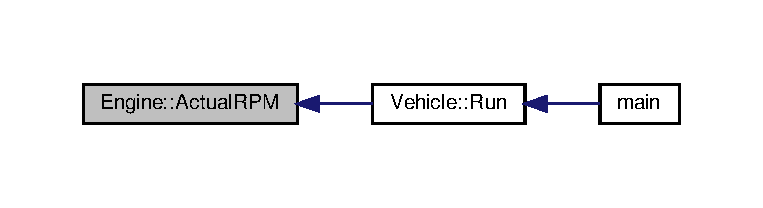
\includegraphics[width=350pt]{classEngine_a72bbd11160a8d916332b26e294133684_icgraph}
\end{center}
\end{figure}
\mbox{\Hypertarget{classEngine_a31646756334221f7967a114c64f188f4}\label{classEngine_a31646756334221f7967a114c64f188f4}} 
\index{Engine@{Engine}!get\+\_\+eng\+\_\+rpm@{get\+\_\+eng\+\_\+rpm}}
\index{get\+\_\+eng\+\_\+rpm@{get\+\_\+eng\+\_\+rpm}!Engine@{Engine}}
\subsubsection{\texorpdfstring{get\+\_\+eng\+\_\+rpm()}{get\_eng\_rpm()}}
{\footnotesize\ttfamily float Engine\+::get\+\_\+eng\+\_\+rpm (\begin{DoxyParamCaption}{ }\end{DoxyParamCaption})}

Get function for engine R\+PM. \begin{DoxyReturn}{Returns}
current R\+P\+M.\+temp\+\_\+float\+\_\+rpm 
\end{DoxyReturn}
Here is the caller graph for this function\+:
\nopagebreak
\begin{figure}[H]
\begin{center}
\leavevmode
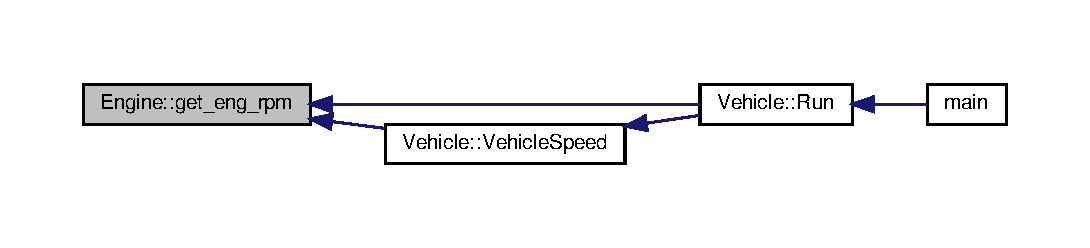
\includegraphics[width=350pt]{classEngine_a31646756334221f7967a114c64f188f4_icgraph}
\end{center}
\end{figure}
\mbox{\Hypertarget{classEngine_abf40022906338faef233d44a93ea01af}\label{classEngine_abf40022906338faef233d44a93ea01af}} 
\index{Engine@{Engine}!get\+\_\+eng\+\_\+sts@{get\+\_\+eng\+\_\+sts}}
\index{get\+\_\+eng\+\_\+sts@{get\+\_\+eng\+\_\+sts}!Engine@{Engine}}
\subsubsection{\texorpdfstring{get\+\_\+eng\+\_\+sts()}{get\_eng\_sts()}}
{\footnotesize\ttfamily bool Engine\+::get\+\_\+eng\+\_\+sts (\begin{DoxyParamCaption}{ }\end{DoxyParamCaption})}

Get function for engine status. \begin{DoxyReturn}{Returns}
current engine status. 
\end{DoxyReturn}
Here is the caller graph for this function\+:
\nopagebreak
\begin{figure}[H]
\begin{center}
\leavevmode
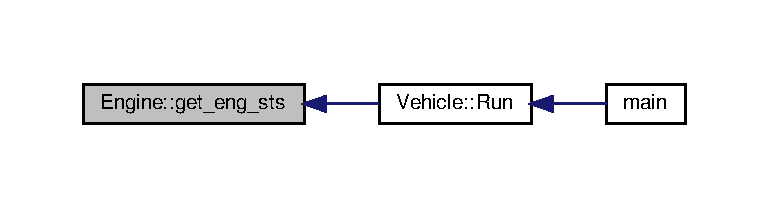
\includegraphics[width=350pt]{classEngine_abf40022906338faef233d44a93ea01af_icgraph}
\end{center}
\end{figure}
\mbox{\Hypertarget{classEngine_a7e4b7cfcb9184beb80fed0ea60a3aad1}\label{classEngine_a7e4b7cfcb9184beb80fed0ea60a3aad1}} 
\index{Engine@{Engine}!Ignition@{Ignition}}
\index{Ignition@{Ignition}!Engine@{Engine}}
\subsubsection{\texorpdfstring{Ignition()}{Ignition()}}
{\footnotesize\ttfamily void Engine\+::\+Ignition (\begin{DoxyParamCaption}\item[{const bool \&}]{ign\+\_\+req,  }\item[{const uint8\+\_\+t \&}]{speed,  }\item[{const uint8\+\_\+t \&}]{brk\+\_\+pedal,  }\item[{const uint8\+\_\+t \&}]{gear\+\_\+position }\end{DoxyParamCaption})}

Determines if engine should be on or off. 
\begin{DoxyParams}{Parameters}
{\em ign\+\_\+req} & ignition request from user. \\
\hline
{\em speed} & current vehicle speed. \\
\hline
{\em brk\+\_\+pedal} & \% that the brake pedal is pressed. \\
\hline
{\em gear\+\_\+position} & current gear lever position. \\
\hline
\end{DoxyParams}
Here is the caller graph for this function\+:
\nopagebreak
\begin{figure}[H]
\begin{center}
\leavevmode
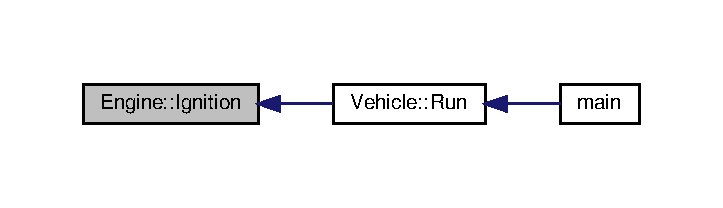
\includegraphics[width=347pt]{classEngine_a7e4b7cfcb9184beb80fed0ea60a3aad1_icgraph}
\end{center}
\end{figure}
\mbox{\Hypertarget{classEngine_aaeaf10a957802225b43d088b5c2ce54b}\label{classEngine_aaeaf10a957802225b43d088b5c2ce54b}} 
\index{Engine@{Engine}!R\+PM@{R\+PM}}
\index{R\+PM@{R\+PM}!Engine@{Engine}}
\subsubsection{\texorpdfstring{R\+P\+M()}{RPM()}}
{\footnotesize\ttfamily void Engine\+::\+R\+PM (\begin{DoxyParamCaption}\item[{const uint8\+\_\+t \&}]{acc\+\_\+pedal,  }\item[{const uint8\+\_\+t \&}]{brk\+\_\+pedal,  }\item[{const uint16\+\_\+t \&}]{sampletime }\end{DoxyParamCaption})}

Increases R\+PM based on user input. Checks that we dont exceed max R\+PM. 
\begin{DoxyParams}{Parameters}
{\em acc\+\_\+pedal} & \% that the acceleration pedal is pressed. \\
\hline
{\em brk\+\_\+pedal} & \% that the brake pedal is pressed. \\
\hline
\end{DoxyParams}
Here is the caller graph for this function\+:
\nopagebreak
\begin{figure}[H]
\begin{center}
\leavevmode
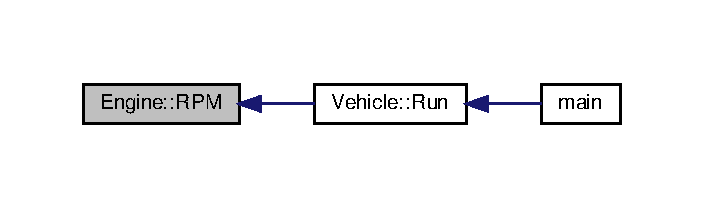
\includegraphics[width=338pt]{classEngine_aaeaf10a957802225b43d088b5c2ce54b_icgraph}
\end{center}
\end{figure}


\subsection{Member Data Documentation}
\mbox{\Hypertarget{classEngine_a450f51a16e7aa1af382193e8acf6e36a}\label{classEngine_a450f51a16e7aa1af382193e8acf6e36a}} 
\index{Engine@{Engine}!eng\+\_\+hp@{eng\+\_\+hp}}
\index{eng\+\_\+hp@{eng\+\_\+hp}!Engine@{Engine}}
\subsubsection{\texorpdfstring{eng\+\_\+hp}{eng\_hp}}
{\footnotesize\ttfamily uint16\+\_\+t Engine\+::eng\+\_\+hp\hspace{0.3cm}{\ttfamily [private]}}

\mbox{\Hypertarget{classEngine_a4a099af57c5bb8df6006aeab0e1f30ae}\label{classEngine_a4a099af57c5bb8df6006aeab0e1f30ae}} 
\index{Engine@{Engine}!eng\+\_\+idle\+\_\+rpm@{eng\+\_\+idle\+\_\+rpm}}
\index{eng\+\_\+idle\+\_\+rpm@{eng\+\_\+idle\+\_\+rpm}!Engine@{Engine}}
\subsubsection{\texorpdfstring{eng\+\_\+idle\+\_\+rpm}{eng\_idle\_rpm}}
{\footnotesize\ttfamily const uint16\+\_\+t Engine\+::eng\+\_\+idle\+\_\+rpm = 900\hspace{0.3cm}{\ttfamily [private]}}

\mbox{\Hypertarget{classEngine_a2d840eecfbd0cc30d0063daee122b66f}\label{classEngine_a2d840eecfbd0cc30d0063daee122b66f}} 
\index{Engine@{Engine}!eng\+\_\+max\+\_\+rpm@{eng\+\_\+max\+\_\+rpm}}
\index{eng\+\_\+max\+\_\+rpm@{eng\+\_\+max\+\_\+rpm}!Engine@{Engine}}
\subsubsection{\texorpdfstring{eng\+\_\+max\+\_\+rpm}{eng\_max\_rpm}}
{\footnotesize\ttfamily uint16\+\_\+t Engine\+::eng\+\_\+max\+\_\+rpm\hspace{0.3cm}{\ttfamily [private]}}

\mbox{\Hypertarget{classEngine_a83b157d748ed627fbeb06ae4a7b4514a}\label{classEngine_a83b157d748ed627fbeb06ae4a7b4514a}} 
\index{Engine@{Engine}!eng\+\_\+min\+\_\+rpm@{eng\+\_\+min\+\_\+rpm}}
\index{eng\+\_\+min\+\_\+rpm@{eng\+\_\+min\+\_\+rpm}!Engine@{Engine}}
\subsubsection{\texorpdfstring{eng\+\_\+min\+\_\+rpm}{eng\_min\_rpm}}
{\footnotesize\ttfamily const uint16\+\_\+t Engine\+::eng\+\_\+min\+\_\+rpm = 850\hspace{0.3cm}{\ttfamily [private]}}

\mbox{\Hypertarget{classEngine_aa502de3162f10d4e7f086cb08c817372}\label{classEngine_aa502de3162f10d4e7f086cb08c817372}} 
\index{Engine@{Engine}!eng\+\_\+rpm@{eng\+\_\+rpm}}
\index{eng\+\_\+rpm@{eng\+\_\+rpm}!Engine@{Engine}}
\subsubsection{\texorpdfstring{eng\+\_\+rpm}{eng\_rpm}}
{\footnotesize\ttfamily float Engine\+::eng\+\_\+rpm\hspace{0.3cm}{\ttfamily [private]}}

\mbox{\Hypertarget{classEngine_a2c5cddbb86ed53703f2ed8182d505c82}\label{classEngine_a2c5cddbb86ed53703f2ed8182d505c82}} 
\index{Engine@{Engine}!eng\+\_\+sts@{eng\+\_\+sts}}
\index{eng\+\_\+sts@{eng\+\_\+sts}!Engine@{Engine}}
\subsubsection{\texorpdfstring{eng\+\_\+sts}{eng\_sts}}
{\footnotesize\ttfamily bool Engine\+::eng\+\_\+sts\hspace{0.3cm}{\ttfamily [private]}}

\mbox{\Hypertarget{classEngine_ac03e3994b854b6ecbb3bf05dba2942a5}\label{classEngine_ac03e3994b854b6ecbb3bf05dba2942a5}} 
\index{Engine@{Engine}!rpm\+\_\+max\+\_\+dec@{rpm\+\_\+max\+\_\+dec}}
\index{rpm\+\_\+max\+\_\+dec@{rpm\+\_\+max\+\_\+dec}!Engine@{Engine}}
\subsubsection{\texorpdfstring{rpm\+\_\+max\+\_\+dec}{rpm\_max\_dec}}
{\footnotesize\ttfamily const uint16\+\_\+t Engine\+::rpm\+\_\+max\+\_\+dec = 150\hspace{0.3cm}{\ttfamily [private]}}

\mbox{\Hypertarget{classEngine_aac9426589cebccaa8cadf7cc7a0ba9be}\label{classEngine_aac9426589cebccaa8cadf7cc7a0ba9be}} 
\index{Engine@{Engine}!rpm\+\_\+simulation\+\_\+constant@{rpm\+\_\+simulation\+\_\+constant}}
\index{rpm\+\_\+simulation\+\_\+constant@{rpm\+\_\+simulation\+\_\+constant}!Engine@{Engine}}
\subsubsection{\texorpdfstring{rpm\+\_\+simulation\+\_\+constant}{rpm\_simulation\_constant}}
{\footnotesize\ttfamily const float Engine\+::rpm\+\_\+simulation\+\_\+constant = 5$\ast$pow(10,-\/7)\hspace{0.3cm}{\ttfamily [private]}}



The documentation for this class was generated from the following files\+:\begin{DoxyCompactItemize}
\item 
/home/rjohan59/repos/bootcamp\+\_\+course/project/source\+\_\+code/drivetrain/include/\hyperlink{engine__simulator_8h}{engine\+\_\+simulator.\+h}\item 
/home/rjohan59/repos/bootcamp\+\_\+course/project/source\+\_\+code/drivetrain/src/\hyperlink{engine__simulator_8cpp}{engine\+\_\+simulator.\+cpp}\end{DoxyCompactItemize}

\hypertarget{classGearbox}{}\section{Gearbox Class Reference}
\label{classGearbox}\index{Gearbox@{Gearbox}}


{\ttfamily \#include $<$gearbox\+\_\+simulator.\+h$>$}



Collaboration diagram for Gearbox\+:
\nopagebreak
\begin{figure}[H]
\begin{center}
\leavevmode
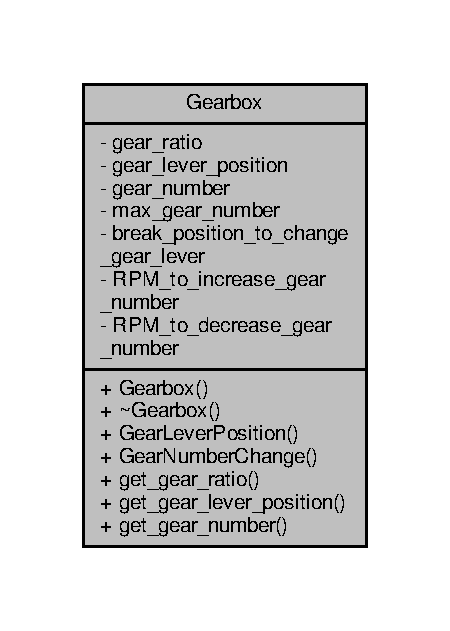
\includegraphics[width=216pt]{classGearbox__coll__graph}
\end{center}
\end{figure}
\subsection*{Public Member Functions}
\begin{DoxyCompactItemize}
\item 
\hyperlink{classGearbox_ad69644f532bef91882a7ee5142072db9}{Gearbox} (double $\ast$\hyperlink{classGearbox_abb63a875027a74947b345a080f012042}{gear\+\_\+ratio}, const uint8\+\_\+t \&gear\+\_\+ratio\+\_\+size)
\item 
\hyperlink{classGearbox_a61e8c826de0c32d2acdfca6710209b11}{$\sim$\+Gearbox} ()=default
\item 
void \hyperlink{classGearbox_aca889116aa57b83145c51a5fe6ca3319}{Gear\+Lever\+Position} (const uint8\+\_\+t \&gear\+\_\+position\+\_\+request, const uint8\+\_\+t \&speed, const uint8\+\_\+t \&brake\+\_\+pedal)
\item 
bool \hyperlink{classGearbox_a7204cb43a9a923283b7d8994e8d1317d}{Gear\+Number\+Change} (const float \&engine\+\_\+rpm)
\item 
double \hyperlink{classGearbox_ad53da0be7891d702873f2a97e0f49c3a}{get\+\_\+gear\+\_\+ratio} ()
\item 
uint8\+\_\+t \hyperlink{classGearbox_a6e3e4eefa42a5811396aee1fad572adc}{get\+\_\+gear\+\_\+lever\+\_\+position} ()
\item 
uint8\+\_\+t \hyperlink{classGearbox_afa81be24e956de8328e32fd1e361eff7}{get\+\_\+gear\+\_\+number} ()
\end{DoxyCompactItemize}
\subsection*{Private Attributes}
\begin{DoxyCompactItemize}
\item 
double $\ast$ \hyperlink{classGearbox_abb63a875027a74947b345a080f012042}{gear\+\_\+ratio}
\item 
uint8\+\_\+t \hyperlink{classGearbox_a1fb7a1973d59b2af8bfd43138c10a087}{gear\+\_\+lever\+\_\+position}
\item 
uint8\+\_\+t \hyperlink{classGearbox_a124962b15e4138b6d5cabbd47e3a85ec}{gear\+\_\+number}
\item 
uint8\+\_\+t \hyperlink{classGearbox_abe090c962b87301623d90d15cf61714c}{max\+\_\+gear\+\_\+number}
\item 
const uint8\+\_\+t \hyperlink{classGearbox_a3b7708c5a08bc9758a5317e59dbea5c9}{break\+\_\+position\+\_\+to\+\_\+change\+\_\+gear\+\_\+lever} = 10
\item 
const uint16\+\_\+t \hyperlink{classGearbox_a7730abcaf967e6b3709ae41bd1827c14}{R\+P\+M\+\_\+to\+\_\+increase\+\_\+gear\+\_\+number} = 6000
\item 
const uint16\+\_\+t \hyperlink{classGearbox_a4c111dfacfef644a60497c22d0b003d5}{R\+P\+M\+\_\+to\+\_\+decrease\+\_\+gear\+\_\+number} = 3500
\end{DoxyCompactItemize}


\subsection{Constructor \& Destructor Documentation}
\mbox{\Hypertarget{classGearbox_ad69644f532bef91882a7ee5142072db9}\label{classGearbox_ad69644f532bef91882a7ee5142072db9}} 
\index{Gearbox@{Gearbox}!Gearbox@{Gearbox}}
\index{Gearbox@{Gearbox}!Gearbox@{Gearbox}}
\subsubsection{\texorpdfstring{Gearbox()}{Gearbox()}}
{\footnotesize\ttfamily Gearbox\+::\+Gearbox (\begin{DoxyParamCaption}\item[{double $\ast$}]{gear\+\_\+ratio,  }\item[{const uint8\+\_\+t \&}]{gear\+\_\+ratio\+\_\+size }\end{DoxyParamCaption})}

Constructor of \hyperlink{classGearbox}{Gearbox}. Assigns the class members. 
\begin{DoxyParams}{Parameters}
{\em gear\+\_\+ratio} & gear ratio for each gear. Index representing the gear where index 0 specifies gear ratio for reverse \\
\hline
{\em gear\+\_\+ratio\+\_\+size} & the number of elements in gear\+\_\+ratio \\
\hline
\end{DoxyParams}
\mbox{\Hypertarget{classGearbox_a61e8c826de0c32d2acdfca6710209b11}\label{classGearbox_a61e8c826de0c32d2acdfca6710209b11}} 
\index{Gearbox@{Gearbox}!````~Gearbox@{$\sim$\+Gearbox}}
\index{````~Gearbox@{$\sim$\+Gearbox}!Gearbox@{Gearbox}}
\subsubsection{\texorpdfstring{$\sim$\+Gearbox()}{~Gearbox()}}
{\footnotesize\ttfamily Gearbox\+::$\sim$\+Gearbox (\begin{DoxyParamCaption}{ }\end{DoxyParamCaption})\hspace{0.3cm}{\ttfamily [default]}}



\subsection{Member Function Documentation}
\mbox{\Hypertarget{classGearbox_aca889116aa57b83145c51a5fe6ca3319}\label{classGearbox_aca889116aa57b83145c51a5fe6ca3319}} 
\index{Gearbox@{Gearbox}!Gear\+Lever\+Position@{Gear\+Lever\+Position}}
\index{Gear\+Lever\+Position@{Gear\+Lever\+Position}!Gearbox@{Gearbox}}
\subsubsection{\texorpdfstring{Gear\+Lever\+Position()}{GearLeverPosition()}}
{\footnotesize\ttfamily void Gearbox\+::\+Gear\+Lever\+Position (\begin{DoxyParamCaption}\item[{const uint8\+\_\+t \&}]{gear\+\_\+position\+\_\+request,  }\item[{const uint8\+\_\+t \&}]{speed,  }\item[{const uint8\+\_\+t \&}]{brake\+\_\+pedal }\end{DoxyParamCaption})}

Checks if a gear lever position switch should be performed. Switches if conditions are fulfilled and sets the gear number. 
\begin{DoxyParams}{Parameters}
{\em gear\+\_\+position\+\_\+request} & gear lever position request by user \\
\hline
{\em speed} & speed of the vehicle \\
\hline
{\em brake\+\_\+pedal} & brake pedal position request by user. 0-\/100\% \\
\hline
\end{DoxyParams}
Here is the caller graph for this function\+:
\nopagebreak
\begin{figure}[H]
\begin{center}
\leavevmode
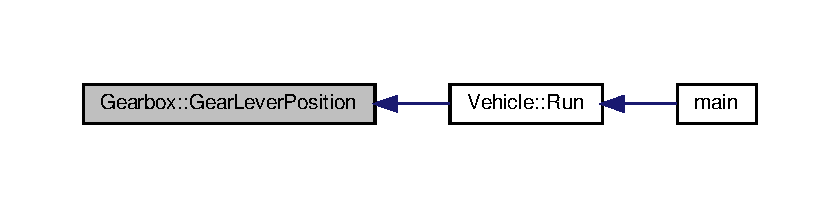
\includegraphics[width=350pt]{classGearbox_aca889116aa57b83145c51a5fe6ca3319_icgraph}
\end{center}
\end{figure}
\mbox{\Hypertarget{classGearbox_a7204cb43a9a923283b7d8994e8d1317d}\label{classGearbox_a7204cb43a9a923283b7d8994e8d1317d}} 
\index{Gearbox@{Gearbox}!Gear\+Number\+Change@{Gear\+Number\+Change}}
\index{Gear\+Number\+Change@{Gear\+Number\+Change}!Gearbox@{Gearbox}}
\subsubsection{\texorpdfstring{Gear\+Number\+Change()}{GearNumberChange()}}
{\footnotesize\ttfamily bool Gearbox\+::\+Gear\+Number\+Change (\begin{DoxyParamCaption}\item[{const float \&}]{engine\+\_\+rpm }\end{DoxyParamCaption})}

Checks if a gear number switch should be performed based on egine R\+PM. Switches if conditions are fulfilled 
\begin{DoxyParams}{Parameters}
{\em engine\+\_\+rpm} & engine R\+PM \\
\hline
\end{DoxyParams}
Here is the caller graph for this function\+:
\nopagebreak
\begin{figure}[H]
\begin{center}
\leavevmode
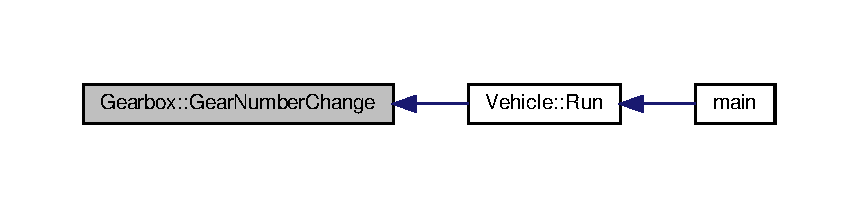
\includegraphics[width=350pt]{classGearbox_a7204cb43a9a923283b7d8994e8d1317d_icgraph}
\end{center}
\end{figure}
\mbox{\Hypertarget{classGearbox_a6e3e4eefa42a5811396aee1fad572adc}\label{classGearbox_a6e3e4eefa42a5811396aee1fad572adc}} 
\index{Gearbox@{Gearbox}!get\+\_\+gear\+\_\+lever\+\_\+position@{get\+\_\+gear\+\_\+lever\+\_\+position}}
\index{get\+\_\+gear\+\_\+lever\+\_\+position@{get\+\_\+gear\+\_\+lever\+\_\+position}!Gearbox@{Gearbox}}
\subsubsection{\texorpdfstring{get\+\_\+gear\+\_\+lever\+\_\+position()}{get\_gear\_lever\_position()}}
{\footnotesize\ttfamily uint8\+\_\+t Gearbox\+::get\+\_\+gear\+\_\+lever\+\_\+position (\begin{DoxyParamCaption}{ }\end{DoxyParamCaption})}

Get function for gear lever position (P = 0, N = 1, D = 2, R = 3) \begin{DoxyReturn}{Returns}
engaged gear lever position 
\end{DoxyReturn}
Here is the caller graph for this function\+:
\nopagebreak
\begin{figure}[H]
\begin{center}
\leavevmode
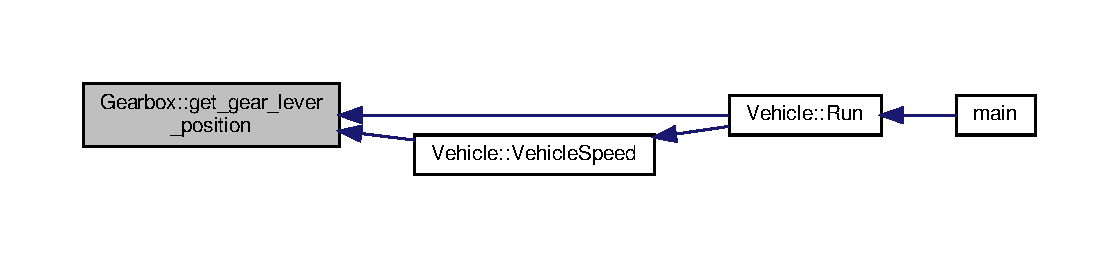
\includegraphics[width=350pt]{classGearbox_a6e3e4eefa42a5811396aee1fad572adc_icgraph}
\end{center}
\end{figure}
\mbox{\Hypertarget{classGearbox_afa81be24e956de8328e32fd1e361eff7}\label{classGearbox_afa81be24e956de8328e32fd1e361eff7}} 
\index{Gearbox@{Gearbox}!get\+\_\+gear\+\_\+number@{get\+\_\+gear\+\_\+number}}
\index{get\+\_\+gear\+\_\+number@{get\+\_\+gear\+\_\+number}!Gearbox@{Gearbox}}
\subsubsection{\texorpdfstring{get\+\_\+gear\+\_\+number()}{get\_gear\_number()}}
{\footnotesize\ttfamily uint8\+\_\+t Gearbox\+::get\+\_\+gear\+\_\+number (\begin{DoxyParamCaption}{ }\end{DoxyParamCaption})}

Get function for gear number (1, 2, 3, ...) \begin{DoxyReturn}{Returns}
engaged gear number 
\end{DoxyReturn}
Here is the caller graph for this function\+:
\nopagebreak
\begin{figure}[H]
\begin{center}
\leavevmode
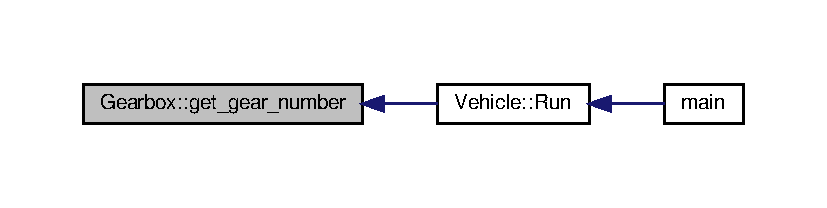
\includegraphics[width=350pt]{classGearbox_afa81be24e956de8328e32fd1e361eff7_icgraph}
\end{center}
\end{figure}
\mbox{\Hypertarget{classGearbox_ad53da0be7891d702873f2a97e0f49c3a}\label{classGearbox_ad53da0be7891d702873f2a97e0f49c3a}} 
\index{Gearbox@{Gearbox}!get\+\_\+gear\+\_\+ratio@{get\+\_\+gear\+\_\+ratio}}
\index{get\+\_\+gear\+\_\+ratio@{get\+\_\+gear\+\_\+ratio}!Gearbox@{Gearbox}}
\subsubsection{\texorpdfstring{get\+\_\+gear\+\_\+ratio()}{get\_gear\_ratio()}}
{\footnotesize\ttfamily double Gearbox\+::get\+\_\+gear\+\_\+ratio (\begin{DoxyParamCaption}{ }\end{DoxyParamCaption})}

Get function for gear ratio. \begin{DoxyReturn}{Returns}
gear ratio for the engaged gear number 
\end{DoxyReturn}
Here is the caller graph for this function\+:
\nopagebreak
\begin{figure}[H]
\begin{center}
\leavevmode
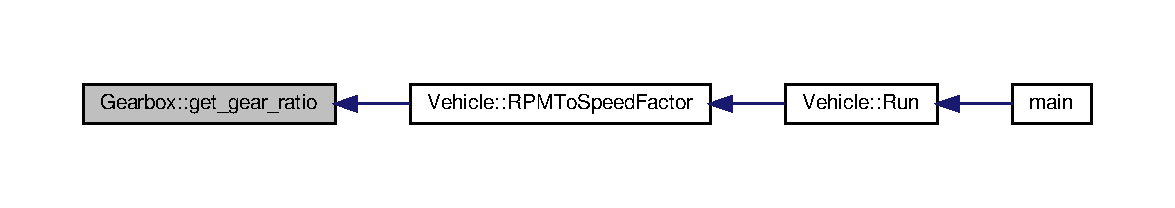
\includegraphics[width=350pt]{classGearbox_ad53da0be7891d702873f2a97e0f49c3a_icgraph}
\end{center}
\end{figure}


\subsection{Member Data Documentation}
\mbox{\Hypertarget{classGearbox_a3b7708c5a08bc9758a5317e59dbea5c9}\label{classGearbox_a3b7708c5a08bc9758a5317e59dbea5c9}} 
\index{Gearbox@{Gearbox}!break\+\_\+position\+\_\+to\+\_\+change\+\_\+gear\+\_\+lever@{break\+\_\+position\+\_\+to\+\_\+change\+\_\+gear\+\_\+lever}}
\index{break\+\_\+position\+\_\+to\+\_\+change\+\_\+gear\+\_\+lever@{break\+\_\+position\+\_\+to\+\_\+change\+\_\+gear\+\_\+lever}!Gearbox@{Gearbox}}
\subsubsection{\texorpdfstring{break\+\_\+position\+\_\+to\+\_\+change\+\_\+gear\+\_\+lever}{break\_position\_to\_change\_gear\_lever}}
{\footnotesize\ttfamily const uint8\+\_\+t Gearbox\+::break\+\_\+position\+\_\+to\+\_\+change\+\_\+gear\+\_\+lever = 10\hspace{0.3cm}{\ttfamily [private]}}

\mbox{\Hypertarget{classGearbox_a1fb7a1973d59b2af8bfd43138c10a087}\label{classGearbox_a1fb7a1973d59b2af8bfd43138c10a087}} 
\index{Gearbox@{Gearbox}!gear\+\_\+lever\+\_\+position@{gear\+\_\+lever\+\_\+position}}
\index{gear\+\_\+lever\+\_\+position@{gear\+\_\+lever\+\_\+position}!Gearbox@{Gearbox}}
\subsubsection{\texorpdfstring{gear\+\_\+lever\+\_\+position}{gear\_lever\_position}}
{\footnotesize\ttfamily uint8\+\_\+t Gearbox\+::gear\+\_\+lever\+\_\+position\hspace{0.3cm}{\ttfamily [private]}}

\mbox{\Hypertarget{classGearbox_a124962b15e4138b6d5cabbd47e3a85ec}\label{classGearbox_a124962b15e4138b6d5cabbd47e3a85ec}} 
\index{Gearbox@{Gearbox}!gear\+\_\+number@{gear\+\_\+number}}
\index{gear\+\_\+number@{gear\+\_\+number}!Gearbox@{Gearbox}}
\subsubsection{\texorpdfstring{gear\+\_\+number}{gear\_number}}
{\footnotesize\ttfamily uint8\+\_\+t Gearbox\+::gear\+\_\+number\hspace{0.3cm}{\ttfamily [private]}}

\mbox{\Hypertarget{classGearbox_abb63a875027a74947b345a080f012042}\label{classGearbox_abb63a875027a74947b345a080f012042}} 
\index{Gearbox@{Gearbox}!gear\+\_\+ratio@{gear\+\_\+ratio}}
\index{gear\+\_\+ratio@{gear\+\_\+ratio}!Gearbox@{Gearbox}}
\subsubsection{\texorpdfstring{gear\+\_\+ratio}{gear\_ratio}}
{\footnotesize\ttfamily double$\ast$ Gearbox\+::gear\+\_\+ratio\hspace{0.3cm}{\ttfamily [private]}}

\mbox{\Hypertarget{classGearbox_abe090c962b87301623d90d15cf61714c}\label{classGearbox_abe090c962b87301623d90d15cf61714c}} 
\index{Gearbox@{Gearbox}!max\+\_\+gear\+\_\+number@{max\+\_\+gear\+\_\+number}}
\index{max\+\_\+gear\+\_\+number@{max\+\_\+gear\+\_\+number}!Gearbox@{Gearbox}}
\subsubsection{\texorpdfstring{max\+\_\+gear\+\_\+number}{max\_gear\_number}}
{\footnotesize\ttfamily uint8\+\_\+t Gearbox\+::max\+\_\+gear\+\_\+number\hspace{0.3cm}{\ttfamily [private]}}

\mbox{\Hypertarget{classGearbox_a4c111dfacfef644a60497c22d0b003d5}\label{classGearbox_a4c111dfacfef644a60497c22d0b003d5}} 
\index{Gearbox@{Gearbox}!R\+P\+M\+\_\+to\+\_\+decrease\+\_\+gear\+\_\+number@{R\+P\+M\+\_\+to\+\_\+decrease\+\_\+gear\+\_\+number}}
\index{R\+P\+M\+\_\+to\+\_\+decrease\+\_\+gear\+\_\+number@{R\+P\+M\+\_\+to\+\_\+decrease\+\_\+gear\+\_\+number}!Gearbox@{Gearbox}}
\subsubsection{\texorpdfstring{R\+P\+M\+\_\+to\+\_\+decrease\+\_\+gear\+\_\+number}{RPM\_to\_decrease\_gear\_number}}
{\footnotesize\ttfamily const uint16\+\_\+t Gearbox\+::\+R\+P\+M\+\_\+to\+\_\+decrease\+\_\+gear\+\_\+number = 3500\hspace{0.3cm}{\ttfamily [private]}}

\mbox{\Hypertarget{classGearbox_a7730abcaf967e6b3709ae41bd1827c14}\label{classGearbox_a7730abcaf967e6b3709ae41bd1827c14}} 
\index{Gearbox@{Gearbox}!R\+P\+M\+\_\+to\+\_\+increase\+\_\+gear\+\_\+number@{R\+P\+M\+\_\+to\+\_\+increase\+\_\+gear\+\_\+number}}
\index{R\+P\+M\+\_\+to\+\_\+increase\+\_\+gear\+\_\+number@{R\+P\+M\+\_\+to\+\_\+increase\+\_\+gear\+\_\+number}!Gearbox@{Gearbox}}
\subsubsection{\texorpdfstring{R\+P\+M\+\_\+to\+\_\+increase\+\_\+gear\+\_\+number}{RPM\_to\_increase\_gear\_number}}
{\footnotesize\ttfamily const uint16\+\_\+t Gearbox\+::\+R\+P\+M\+\_\+to\+\_\+increase\+\_\+gear\+\_\+number = 6000\hspace{0.3cm}{\ttfamily [private]}}



The documentation for this class was generated from the following files\+:\begin{DoxyCompactItemize}
\item 
/home/rjohan59/repos/bootcamp\+\_\+course/project/source\+\_\+code/drivetrain/include/\hyperlink{gearbox__simulator_8h}{gearbox\+\_\+simulator.\+h}\item 
/home/rjohan59/repos/bootcamp\+\_\+course/project/source\+\_\+code/drivetrain/src/\hyperlink{gearbox__simulator_8cpp}{gearbox\+\_\+simulator.\+cpp}\end{DoxyCompactItemize}

\hypertarget{classInputReader}{}\section{Input\+Reader Class Reference}
\label{classInputReader}\index{Input\+Reader@{Input\+Reader}}


{\ttfamily \#include $<$keyboard\+\_\+input\+\_\+reader.\+h$>$}



Collaboration diagram for Input\+Reader\+:
\nopagebreak
\begin{figure}[H]
\begin{center}
\leavevmode
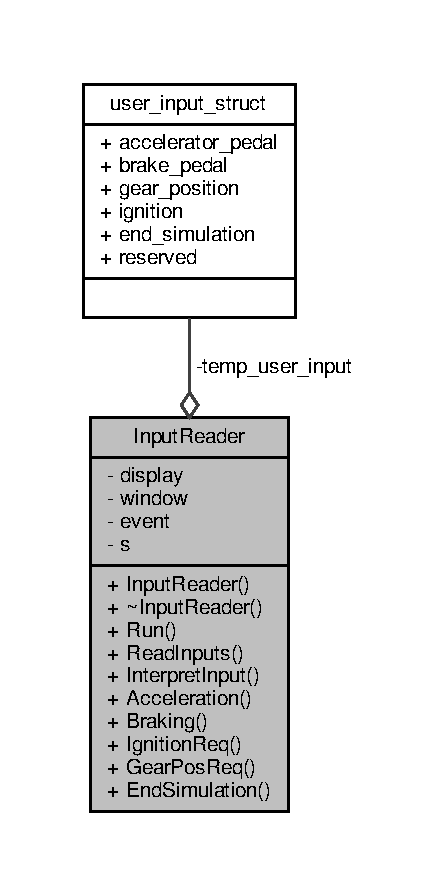
\includegraphics[width=210pt]{classInputReader__coll__graph}
\end{center}
\end{figure}
\subsection*{Public Member Functions}
\begin{DoxyCompactItemize}
\item 
\hyperlink{classInputReader_ae7d7eaec9edd0b8a5e6c5870f23070c3}{Input\+Reader} ()
\item 
\hyperlink{classInputReader_a38875ce3bae818dd0836da36fb7ea891}{$\sim$\+Input\+Reader} ()
\item 
bool \hyperlink{classInputReader_a258e1e58806e172a4339bb2aec9a85f0}{Run} ()
\item 
bool \hyperlink{classInputReader_a541f5d60fa0d9ee786d82f1541485a4a}{Read\+Inputs} ()
\item 
bool \hyperlink{classInputReader_a83a83d74ccb7cd6a29da3b558babaf1c}{Interpret\+Input} ()
\item 
void \hyperlink{classInputReader_a0740495343639fcf0759a1b8fe0fe2e0}{Acceleration} ()
\item 
void \hyperlink{classInputReader_ad35d36c2bac3f4b6bae2d2ad501873cb}{Braking} ()
\item 
void \hyperlink{classInputReader_a0a4c53621f5b7c8e3373341c1f383001}{Ignition\+Req} ()
\item 
void \hyperlink{classInputReader_aec41f6307eb1f4ca8308d4f002ce1cf0}{Gear\+Pos\+Req} ()
\item 
bool \hyperlink{classInputReader_af314d9877257c41a41d937e3ca00c679}{End\+Simulation} ()
\end{DoxyCompactItemize}
\subsection*{Private Attributes}
\begin{DoxyCompactItemize}
\item 
\hyperlink{user__input_8h_a4be483183ef50f2de9cefcb22df23699}{User\+Input} \hyperlink{classInputReader_ad19bb2b46ab677724d4fe3352cab13d6}{temp\+\_\+user\+\_\+input}
\item 
Display $\ast$ \hyperlink{classInputReader_ac8b258254da835100455ef83dd3921df}{display}
\item 
Window \hyperlink{classInputReader_aa27cb19e6c3d1fa1d968b798b5aaa6c5}{window}
\item 
X\+Event \hyperlink{classInputReader_a737042e6b612b74a6444d611297af66f}{event}
\item 
int \hyperlink{classInputReader_af8a0467bf9ab4a7e054eb46b77adf96a}{s}
\end{DoxyCompactItemize}


\subsection{Constructor \& Destructor Documentation}
\mbox{\Hypertarget{classInputReader_ae7d7eaec9edd0b8a5e6c5870f23070c3}\label{classInputReader_ae7d7eaec9edd0b8a5e6c5870f23070c3}} 
\index{Input\+Reader@{Input\+Reader}!Input\+Reader@{Input\+Reader}}
\index{Input\+Reader@{Input\+Reader}!Input\+Reader@{Input\+Reader}}
\subsubsection{\texorpdfstring{Input\+Reader()}{InputReader()}}
{\footnotesize\ttfamily Input\+Reader\+::\+Input\+Reader (\begin{DoxyParamCaption}{ }\end{DoxyParamCaption})}

Constructor for class \hyperlink{classInputReader}{Input\+Reader}, opens a display and changes settings wanted for the keyboard reading. Sets temp\+\_\+user\+\_\+input struct to 0 and adds it to the C\+AN buffer. \begin{DoxyReturn}{Returns}
Nothing is returned 
\end{DoxyReturn}
Here is the call graph for this function\+:
\nopagebreak
\begin{figure}[H]
\begin{center}
\leavevmode
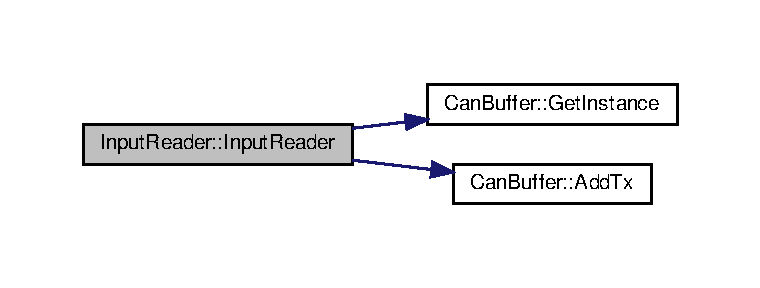
\includegraphics[width=350pt]{classInputReader_ae7d7eaec9edd0b8a5e6c5870f23070c3_cgraph}
\end{center}
\end{figure}
\mbox{\Hypertarget{classInputReader_a38875ce3bae818dd0836da36fb7ea891}\label{classInputReader_a38875ce3bae818dd0836da36fb7ea891}} 
\index{Input\+Reader@{Input\+Reader}!````~Input\+Reader@{$\sim$\+Input\+Reader}}
\index{````~Input\+Reader@{$\sim$\+Input\+Reader}!Input\+Reader@{Input\+Reader}}
\subsubsection{\texorpdfstring{$\sim$\+Input\+Reader()}{~InputReader()}}
{\footnotesize\ttfamily Input\+Reader\+::$\sim$\+Input\+Reader (\begin{DoxyParamCaption}{ }\end{DoxyParamCaption})}

Destructor for class \hyperlink{classInputReader}{Input\+Reader}, closes the display and resets settings for the keyboard. \begin{DoxyReturn}{Returns}
Nothing is returned 
\end{DoxyReturn}


\subsection{Member Function Documentation}
\mbox{\Hypertarget{classInputReader_a0740495343639fcf0759a1b8fe0fe2e0}\label{classInputReader_a0740495343639fcf0759a1b8fe0fe2e0}} 
\index{Input\+Reader@{Input\+Reader}!Acceleration@{Acceleration}}
\index{Acceleration@{Acceleration}!Input\+Reader@{Input\+Reader}}
\subsubsection{\texorpdfstring{Acceleration()}{Acceleration()}}
{\footnotesize\ttfamily void Input\+Reader\+::\+Acceleration (\begin{DoxyParamCaption}{ }\end{DoxyParamCaption})}

Increases or decreases acceleration value, stores it in temp\+\_\+user\+\_\+input. \begin{DoxyReturn}{Returns}
Nothing is returned. 
\end{DoxyReturn}
Here is the caller graph for this function\+:
\nopagebreak
\begin{figure}[H]
\begin{center}
\leavevmode
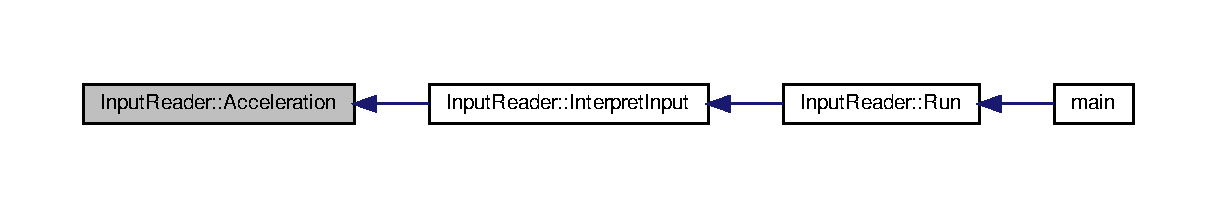
\includegraphics[width=350pt]{classInputReader_a0740495343639fcf0759a1b8fe0fe2e0_icgraph}
\end{center}
\end{figure}
\mbox{\Hypertarget{classInputReader_ad35d36c2bac3f4b6bae2d2ad501873cb}\label{classInputReader_ad35d36c2bac3f4b6bae2d2ad501873cb}} 
\index{Input\+Reader@{Input\+Reader}!Braking@{Braking}}
\index{Braking@{Braking}!Input\+Reader@{Input\+Reader}}
\subsubsection{\texorpdfstring{Braking()}{Braking()}}
{\footnotesize\ttfamily void Input\+Reader\+::\+Braking (\begin{DoxyParamCaption}{ }\end{DoxyParamCaption})}

Increases or decreases brake value, stores it in temp\+\_\+user\+\_\+input. \begin{DoxyReturn}{Returns}
Nothing is returned. 
\end{DoxyReturn}
Here is the caller graph for this function\+:
\nopagebreak
\begin{figure}[H]
\begin{center}
\leavevmode
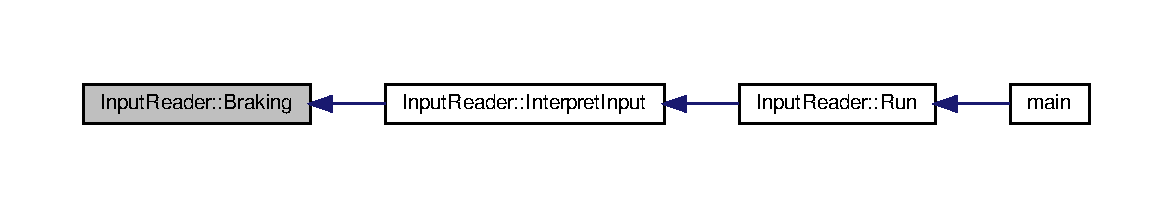
\includegraphics[width=350pt]{classInputReader_ad35d36c2bac3f4b6bae2d2ad501873cb_icgraph}
\end{center}
\end{figure}
\mbox{\Hypertarget{classInputReader_af314d9877257c41a41d937e3ca00c679}\label{classInputReader_af314d9877257c41a41d937e3ca00c679}} 
\index{Input\+Reader@{Input\+Reader}!End\+Simulation@{End\+Simulation}}
\index{End\+Simulation@{End\+Simulation}!Input\+Reader@{Input\+Reader}}
\subsubsection{\texorpdfstring{End\+Simulation()}{EndSimulation()}}
{\footnotesize\ttfamily bool Input\+Reader\+::\+End\+Simulation (\begin{DoxyParamCaption}{ }\end{DoxyParamCaption})}

Sets end simulation. \begin{DoxyReturn}{Returns}
Returns false. 
\end{DoxyReturn}
Here is the caller graph for this function\+:
\nopagebreak
\begin{figure}[H]
\begin{center}
\leavevmode
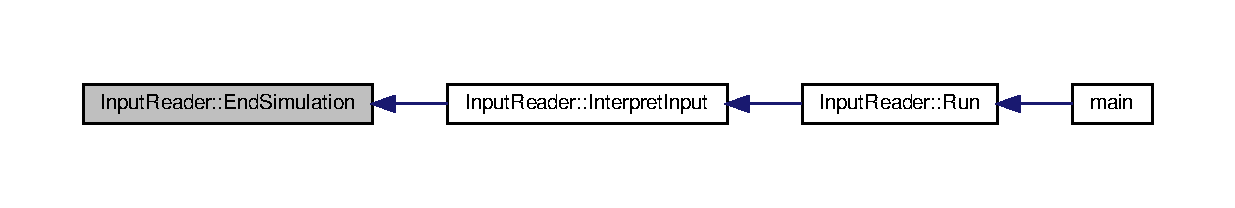
\includegraphics[width=350pt]{classInputReader_af314d9877257c41a41d937e3ca00c679_icgraph}
\end{center}
\end{figure}
\mbox{\Hypertarget{classInputReader_aec41f6307eb1f4ca8308d4f002ce1cf0}\label{classInputReader_aec41f6307eb1f4ca8308d4f002ce1cf0}} 
\index{Input\+Reader@{Input\+Reader}!Gear\+Pos\+Req@{Gear\+Pos\+Req}}
\index{Gear\+Pos\+Req@{Gear\+Pos\+Req}!Input\+Reader@{Input\+Reader}}
\subsubsection{\texorpdfstring{Gear\+Pos\+Req()}{GearPosReq()}}
{\footnotesize\ttfamily void Input\+Reader\+::\+Gear\+Pos\+Req (\begin{DoxyParamCaption}{ }\end{DoxyParamCaption})}

Determines which gear should be requested, stores it in temp\+\_\+user\+\_\+input. \begin{DoxyReturn}{Returns}
Nothing is returned. 
\end{DoxyReturn}
Here is the caller graph for this function\+:
\nopagebreak
\begin{figure}[H]
\begin{center}
\leavevmode
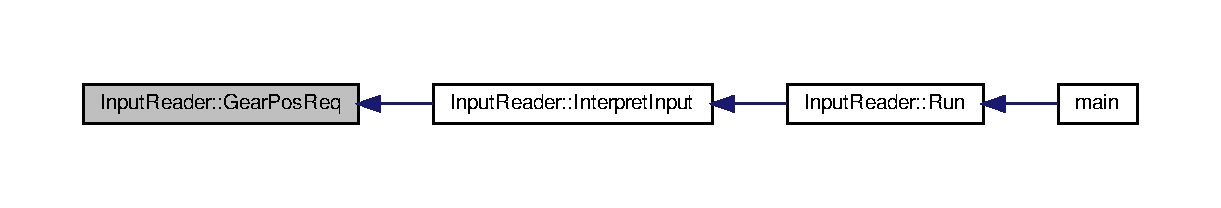
\includegraphics[width=350pt]{classInputReader_aec41f6307eb1f4ca8308d4f002ce1cf0_icgraph}
\end{center}
\end{figure}
\mbox{\Hypertarget{classInputReader_a0a4c53621f5b7c8e3373341c1f383001}\label{classInputReader_a0a4c53621f5b7c8e3373341c1f383001}} 
\index{Input\+Reader@{Input\+Reader}!Ignition\+Req@{Ignition\+Req}}
\index{Ignition\+Req@{Ignition\+Req}!Input\+Reader@{Input\+Reader}}
\subsubsection{\texorpdfstring{Ignition\+Req()}{IgnitionReq()}}
{\footnotesize\ttfamily void Input\+Reader\+::\+Ignition\+Req (\begin{DoxyParamCaption}{ }\end{DoxyParamCaption})}

Toggles the ignition request, stores it in temp\+\_\+user\+\_\+input. \begin{DoxyReturn}{Returns}
Nothing is returned. 
\end{DoxyReturn}
Here is the caller graph for this function\+:
\nopagebreak
\begin{figure}[H]
\begin{center}
\leavevmode
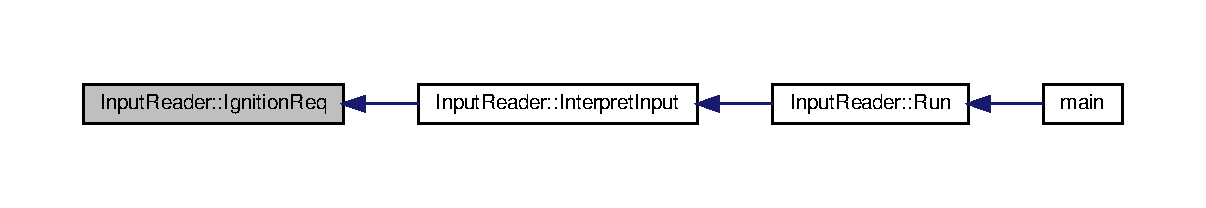
\includegraphics[width=350pt]{classInputReader_a0a4c53621f5b7c8e3373341c1f383001_icgraph}
\end{center}
\end{figure}
\mbox{\Hypertarget{classInputReader_a83a83d74ccb7cd6a29da3b558babaf1c}\label{classInputReader_a83a83d74ccb7cd6a29da3b558babaf1c}} 
\index{Input\+Reader@{Input\+Reader}!Interpret\+Input@{Interpret\+Input}}
\index{Interpret\+Input@{Interpret\+Input}!Input\+Reader@{Input\+Reader}}
\subsubsection{\texorpdfstring{Interpret\+Input()}{InterpretInput()}}
{\footnotesize\ttfamily bool Input\+Reader\+::\+Interpret\+Input (\begin{DoxyParamCaption}{ }\end{DoxyParamCaption})}

Decides appropriate action depending on which key was pressed. \begin{DoxyReturn}{Returns}
Returns true unless Esc key has been pressed. 
\end{DoxyReturn}
Here is the call graph for this function\+:
\nopagebreak
\begin{figure}[H]
\begin{center}
\leavevmode
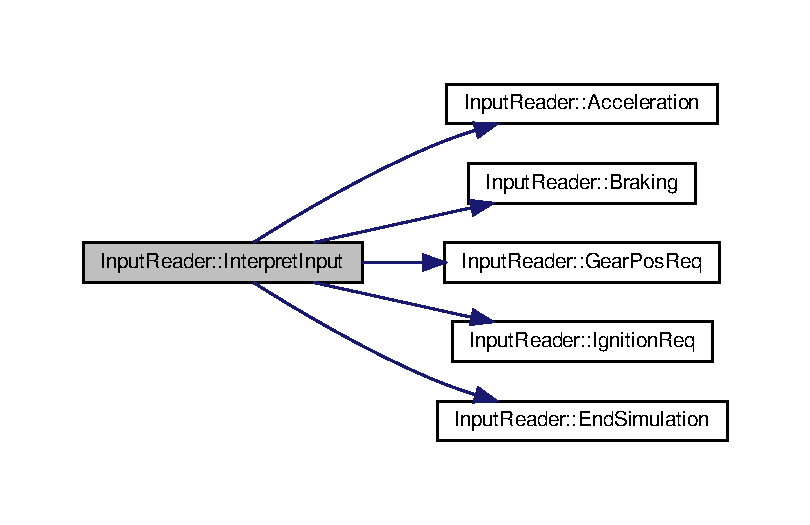
\includegraphics[width=350pt]{classInputReader_a83a83d74ccb7cd6a29da3b558babaf1c_cgraph}
\end{center}
\end{figure}
Here is the caller graph for this function\+:
\nopagebreak
\begin{figure}[H]
\begin{center}
\leavevmode
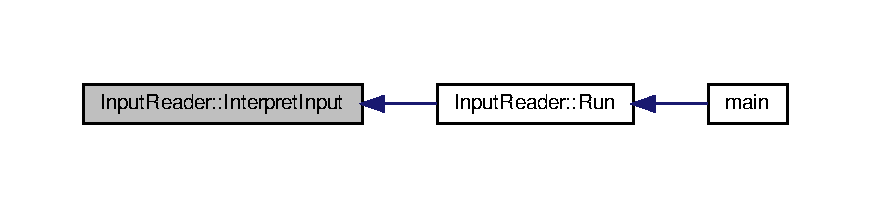
\includegraphics[width=350pt]{classInputReader_a83a83d74ccb7cd6a29da3b558babaf1c_icgraph}
\end{center}
\end{figure}
\mbox{\Hypertarget{classInputReader_a541f5d60fa0d9ee786d82f1541485a4a}\label{classInputReader_a541f5d60fa0d9ee786d82f1541485a4a}} 
\index{Input\+Reader@{Input\+Reader}!Read\+Inputs@{Read\+Inputs}}
\index{Read\+Inputs@{Read\+Inputs}!Input\+Reader@{Input\+Reader}}
\subsubsection{\texorpdfstring{Read\+Inputs()}{ReadInputs()}}
{\footnotesize\ttfamily bool Input\+Reader\+::\+Read\+Inputs (\begin{DoxyParamCaption}{ }\end{DoxyParamCaption})}

Reads inputs from the keyboard (blocking function). \begin{DoxyReturn}{Returns}
True if a Key\+Press has occurred, false for all other events. 
\end{DoxyReturn}
Here is the caller graph for this function\+:
\nopagebreak
\begin{figure}[H]
\begin{center}
\leavevmode
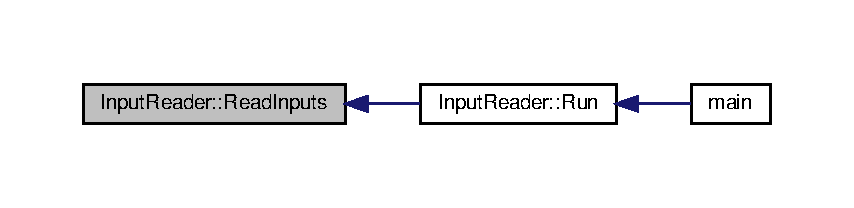
\includegraphics[width=350pt]{classInputReader_a541f5d60fa0d9ee786d82f1541485a4a_icgraph}
\end{center}
\end{figure}
\mbox{\Hypertarget{classInputReader_a258e1e58806e172a4339bb2aec9a85f0}\label{classInputReader_a258e1e58806e172a4339bb2aec9a85f0}} 
\index{Input\+Reader@{Input\+Reader}!Run@{Run}}
\index{Run@{Run}!Input\+Reader@{Input\+Reader}}
\subsubsection{\texorpdfstring{Run()}{Run()}}
{\footnotesize\ttfamily bool Input\+Reader\+::\+Run (\begin{DoxyParamCaption}{ }\end{DoxyParamCaption})}

Runs the main function of \hyperlink{classInputReader}{Input\+Reader}, calls functions Read\+Inputs and Interpret\+Input. Adds a message to \hyperlink{classCanBuffer}{Can\+Buffer} when input has been read and interpreted. \begin{DoxyReturn}{Returns}
Returns True if thread should continue running. 
\end{DoxyReturn}
Here is the call graph for this function\+:
\nopagebreak
\begin{figure}[H]
\begin{center}
\leavevmode
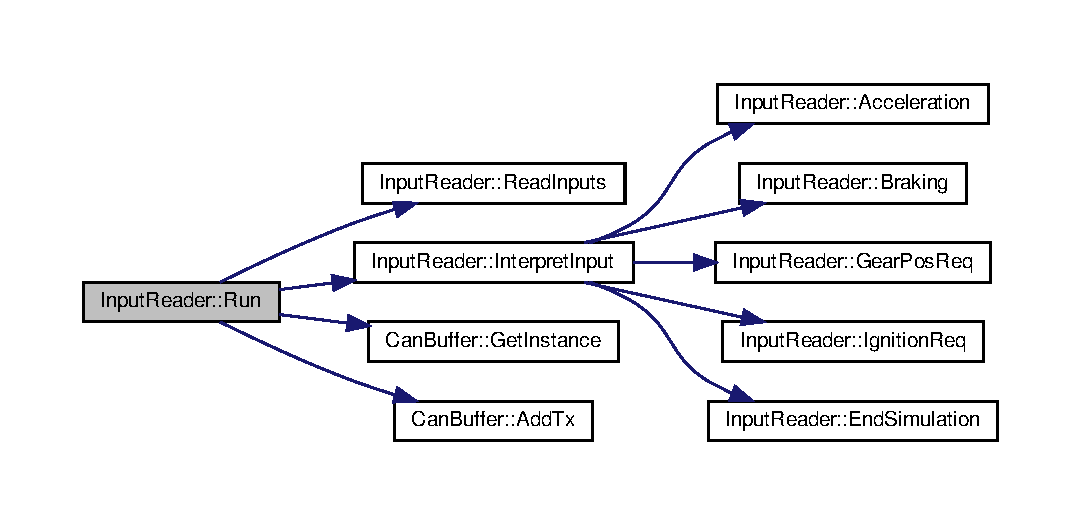
\includegraphics[width=350pt]{classInputReader_a258e1e58806e172a4339bb2aec9a85f0_cgraph}
\end{center}
\end{figure}
Here is the caller graph for this function\+:
\nopagebreak
\begin{figure}[H]
\begin{center}
\leavevmode
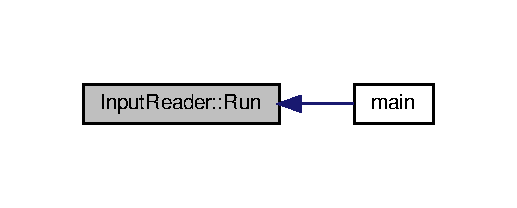
\includegraphics[width=248pt]{classInputReader_a258e1e58806e172a4339bb2aec9a85f0_icgraph}
\end{center}
\end{figure}


\subsection{Member Data Documentation}
\mbox{\Hypertarget{classInputReader_ac8b258254da835100455ef83dd3921df}\label{classInputReader_ac8b258254da835100455ef83dd3921df}} 
\index{Input\+Reader@{Input\+Reader}!display@{display}}
\index{display@{display}!Input\+Reader@{Input\+Reader}}
\subsubsection{\texorpdfstring{display}{display}}
{\footnotesize\ttfamily Display$\ast$ Input\+Reader\+::display\hspace{0.3cm}{\ttfamily [private]}}

\mbox{\Hypertarget{classInputReader_a737042e6b612b74a6444d611297af66f}\label{classInputReader_a737042e6b612b74a6444d611297af66f}} 
\index{Input\+Reader@{Input\+Reader}!event@{event}}
\index{event@{event}!Input\+Reader@{Input\+Reader}}
\subsubsection{\texorpdfstring{event}{event}}
{\footnotesize\ttfamily X\+Event Input\+Reader\+::event\hspace{0.3cm}{\ttfamily [private]}}

\mbox{\Hypertarget{classInputReader_af8a0467bf9ab4a7e054eb46b77adf96a}\label{classInputReader_af8a0467bf9ab4a7e054eb46b77adf96a}} 
\index{Input\+Reader@{Input\+Reader}!s@{s}}
\index{s@{s}!Input\+Reader@{Input\+Reader}}
\subsubsection{\texorpdfstring{s}{s}}
{\footnotesize\ttfamily int Input\+Reader\+::s\hspace{0.3cm}{\ttfamily [private]}}

\mbox{\Hypertarget{classInputReader_ad19bb2b46ab677724d4fe3352cab13d6}\label{classInputReader_ad19bb2b46ab677724d4fe3352cab13d6}} 
\index{Input\+Reader@{Input\+Reader}!temp\+\_\+user\+\_\+input@{temp\+\_\+user\+\_\+input}}
\index{temp\+\_\+user\+\_\+input@{temp\+\_\+user\+\_\+input}!Input\+Reader@{Input\+Reader}}
\subsubsection{\texorpdfstring{temp\+\_\+user\+\_\+input}{temp\_user\_input}}
{\footnotesize\ttfamily \hyperlink{user__input_8h_a4be483183ef50f2de9cefcb22df23699}{User\+Input} Input\+Reader\+::temp\+\_\+user\+\_\+input\hspace{0.3cm}{\ttfamily [private]}}

\mbox{\Hypertarget{classInputReader_aa27cb19e6c3d1fa1d968b798b5aaa6c5}\label{classInputReader_aa27cb19e6c3d1fa1d968b798b5aaa6c5}} 
\index{Input\+Reader@{Input\+Reader}!window@{window}}
\index{window@{window}!Input\+Reader@{Input\+Reader}}
\subsubsection{\texorpdfstring{window}{window}}
{\footnotesize\ttfamily Window Input\+Reader\+::window\hspace{0.3cm}{\ttfamily [private]}}



The documentation for this class was generated from the following files\+:\begin{DoxyCompactItemize}
\item 
/home/rjohan59/repos/bootcamp\+\_\+course/project/source\+\_\+code/input\+\_\+handler/include/\hyperlink{keyboard__input__reader_8h}{keyboard\+\_\+input\+\_\+reader.\+h}\item 
/home/rjohan59/repos/bootcamp\+\_\+course/project/source\+\_\+code/input\+\_\+handler/src/\hyperlink{keyboard__input__reader_8cpp}{keyboard\+\_\+input\+\_\+reader.\+cpp}\end{DoxyCompactItemize}

\hypertarget{classRingbuffer}{}\section{Ringbuffer$<$ T, size $>$ Class Template Reference}
\label{classRingbuffer}\index{Ringbuffer$<$ T, size $>$@{Ringbuffer$<$ T, size $>$}}


{\ttfamily \#include $<$ringbuffer.\+h$>$}



Collaboration diagram for Ringbuffer$<$ T, size $>$\+:
\nopagebreak
\begin{figure}[H]
\begin{center}
\leavevmode
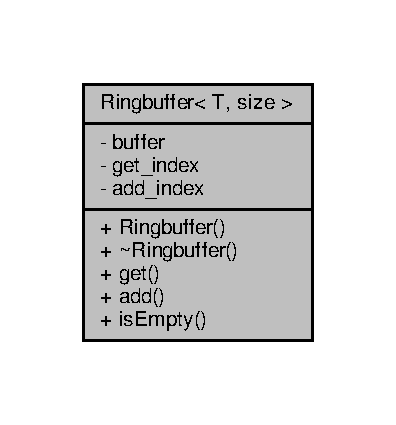
\includegraphics[width=190pt]{classRingbuffer__coll__graph}
\end{center}
\end{figure}
\subsection*{Public Member Functions}
\begin{DoxyCompactItemize}
\item 
\hyperlink{classRingbuffer_a8c05646994076508b9969a06cee6426a}{Ringbuffer} ()=default
\item 
\hyperlink{classRingbuffer_a67242601a0f115e26f221ea2e9ab77e7}{$\sim$\+Ringbuffer} ()
\item 
T \hyperlink{classRingbuffer_a21f95bebbc300f7b7287284ff5a9ea86}{get} ()
\item 
void \hyperlink{classRingbuffer_a88b2aac3e48efb366d16a10746da3420}{add} (T item)
\item 
bool \hyperlink{classRingbuffer_a2ebb965f90ff6a14f184619ef3dfeca6}{is\+Empty} ()
\end{DoxyCompactItemize}
\subsection*{Private Attributes}
\begin{DoxyCompactItemize}
\item 
T $\ast$ \hyperlink{classRingbuffer_a335ecc63190c7e834e1ef5c694c0513a}{buffer} = new T\mbox{[}size\mbox{]}
\item 
size\+\_\+t \hyperlink{classRingbuffer_a36eb74b7c7e5aa2f5804f9565b247306}{get\+\_\+index} = 0
\item 
size\+\_\+t \hyperlink{classRingbuffer_ad4ddec2757f8c74de1107f96a5b99205}{add\+\_\+index} = 0
\end{DoxyCompactItemize}


\subsection{Constructor \& Destructor Documentation}
\mbox{\Hypertarget{classRingbuffer_a8c05646994076508b9969a06cee6426a}\label{classRingbuffer_a8c05646994076508b9969a06cee6426a}} 
\index{Ringbuffer@{Ringbuffer}!Ringbuffer@{Ringbuffer}}
\index{Ringbuffer@{Ringbuffer}!Ringbuffer@{Ringbuffer}}
\subsubsection{\texorpdfstring{Ringbuffer()}{Ringbuffer()}}
{\footnotesize\ttfamily template$<$typename T , size\+\_\+t size = 100$>$ \\
\hyperlink{classRingbuffer}{Ringbuffer}$<$ T, size $>$\+::\hyperlink{classRingbuffer}{Ringbuffer} (\begin{DoxyParamCaption}{ }\end{DoxyParamCaption})\hspace{0.3cm}{\ttfamily [default]}}

\mbox{\Hypertarget{classRingbuffer_a67242601a0f115e26f221ea2e9ab77e7}\label{classRingbuffer_a67242601a0f115e26f221ea2e9ab77e7}} 
\index{Ringbuffer@{Ringbuffer}!````~Ringbuffer@{$\sim$\+Ringbuffer}}
\index{````~Ringbuffer@{$\sim$\+Ringbuffer}!Ringbuffer@{Ringbuffer}}
\subsubsection{\texorpdfstring{$\sim$\+Ringbuffer()}{~Ringbuffer()}}
{\footnotesize\ttfamily template$<$typename T , size\+\_\+t size = 100$>$ \\
\hyperlink{classRingbuffer}{Ringbuffer}$<$ T, size $>$\+::$\sim$\hyperlink{classRingbuffer}{Ringbuffer} (\begin{DoxyParamCaption}{ }\end{DoxyParamCaption})\hspace{0.3cm}{\ttfamily [inline]}}

Here is the call graph for this function\+:
\nopagebreak
\begin{figure}[H]
\begin{center}
\leavevmode
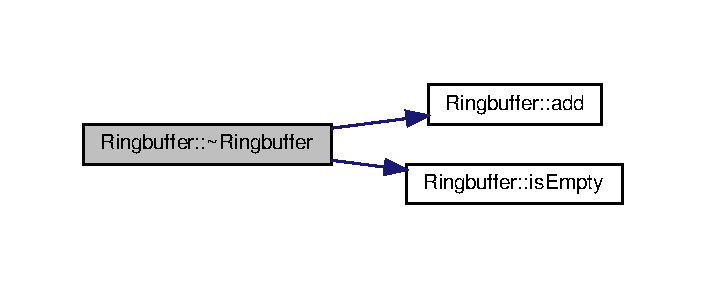
\includegraphics[width=339pt]{classRingbuffer_a67242601a0f115e26f221ea2e9ab77e7_cgraph}
\end{center}
\end{figure}


\subsection{Member Function Documentation}
\mbox{\Hypertarget{classRingbuffer_a88b2aac3e48efb366d16a10746da3420}\label{classRingbuffer_a88b2aac3e48efb366d16a10746da3420}} 
\index{Ringbuffer@{Ringbuffer}!add@{add}}
\index{add@{add}!Ringbuffer@{Ringbuffer}}
\subsubsection{\texorpdfstring{add()}{add()}}
{\footnotesize\ttfamily template$<$typename T , size\+\_\+t size$>$ \\
void \hyperlink{classRingbuffer}{Ringbuffer}$<$ T, size $>$\+::add (\begin{DoxyParamCaption}\item[{T}]{item }\end{DoxyParamCaption})}

Here is the caller graph for this function\+:
\nopagebreak
\begin{figure}[H]
\begin{center}
\leavevmode
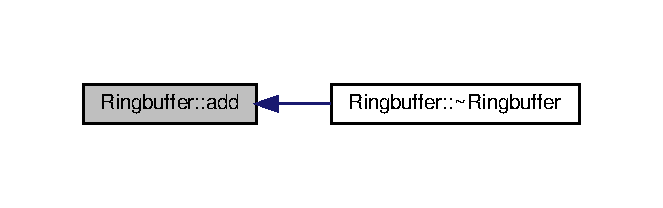
\includegraphics[width=318pt]{classRingbuffer_a88b2aac3e48efb366d16a10746da3420_icgraph}
\end{center}
\end{figure}
\mbox{\Hypertarget{classRingbuffer_a21f95bebbc300f7b7287284ff5a9ea86}\label{classRingbuffer_a21f95bebbc300f7b7287284ff5a9ea86}} 
\index{Ringbuffer@{Ringbuffer}!get@{get}}
\index{get@{get}!Ringbuffer@{Ringbuffer}}
\subsubsection{\texorpdfstring{get()}{get()}}
{\footnotesize\ttfamily template$<$typename T , size\+\_\+t size$>$ \\
T \hyperlink{classRingbuffer}{Ringbuffer}$<$ T, size $>$\+::get (\begin{DoxyParamCaption}{ }\end{DoxyParamCaption})}

\mbox{\Hypertarget{classRingbuffer_a2ebb965f90ff6a14f184619ef3dfeca6}\label{classRingbuffer_a2ebb965f90ff6a14f184619ef3dfeca6}} 
\index{Ringbuffer@{Ringbuffer}!is\+Empty@{is\+Empty}}
\index{is\+Empty@{is\+Empty}!Ringbuffer@{Ringbuffer}}
\subsubsection{\texorpdfstring{is\+Empty()}{isEmpty()}}
{\footnotesize\ttfamily template$<$typename T , size\+\_\+t size = 100$>$ \\
bool \hyperlink{classRingbuffer}{Ringbuffer}$<$ T, size $>$\+::is\+Empty (\begin{DoxyParamCaption}{ }\end{DoxyParamCaption})}

Here is the caller graph for this function\+:
\nopagebreak
\begin{figure}[H]
\begin{center}
\leavevmode
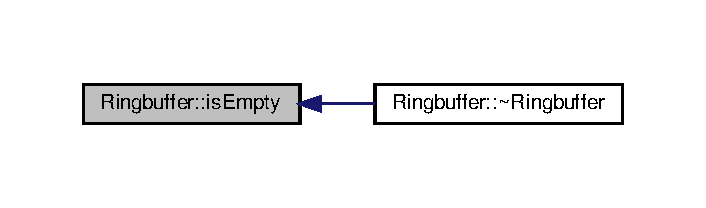
\includegraphics[width=339pt]{classRingbuffer_a2ebb965f90ff6a14f184619ef3dfeca6_icgraph}
\end{center}
\end{figure}


\subsection{Member Data Documentation}
\mbox{\Hypertarget{classRingbuffer_ad4ddec2757f8c74de1107f96a5b99205}\label{classRingbuffer_ad4ddec2757f8c74de1107f96a5b99205}} 
\index{Ringbuffer@{Ringbuffer}!add\+\_\+index@{add\+\_\+index}}
\index{add\+\_\+index@{add\+\_\+index}!Ringbuffer@{Ringbuffer}}
\subsubsection{\texorpdfstring{add\+\_\+index}{add\_index}}
{\footnotesize\ttfamily template$<$typename T , size\+\_\+t size = 100$>$ \\
size\+\_\+t \hyperlink{classRingbuffer}{Ringbuffer}$<$ T, size $>$\+::add\+\_\+index = 0\hspace{0.3cm}{\ttfamily [private]}}

\mbox{\Hypertarget{classRingbuffer_a335ecc63190c7e834e1ef5c694c0513a}\label{classRingbuffer_a335ecc63190c7e834e1ef5c694c0513a}} 
\index{Ringbuffer@{Ringbuffer}!buffer@{buffer}}
\index{buffer@{buffer}!Ringbuffer@{Ringbuffer}}
\subsubsection{\texorpdfstring{buffer}{buffer}}
{\footnotesize\ttfamily template$<$typename T , size\+\_\+t size = 100$>$ \\
T$\ast$ \hyperlink{classRingbuffer}{Ringbuffer}$<$ T, size $>$\+::buffer = new T\mbox{[}size\mbox{]}\hspace{0.3cm}{\ttfamily [private]}}

\mbox{\Hypertarget{classRingbuffer_a36eb74b7c7e5aa2f5804f9565b247306}\label{classRingbuffer_a36eb74b7c7e5aa2f5804f9565b247306}} 
\index{Ringbuffer@{Ringbuffer}!get\+\_\+index@{get\+\_\+index}}
\index{get\+\_\+index@{get\+\_\+index}!Ringbuffer@{Ringbuffer}}
\subsubsection{\texorpdfstring{get\+\_\+index}{get\_index}}
{\footnotesize\ttfamily template$<$typename T , size\+\_\+t size = 100$>$ \\
size\+\_\+t \hyperlink{classRingbuffer}{Ringbuffer}$<$ T, size $>$\+::get\+\_\+index = 0\hspace{0.3cm}{\ttfamily [private]}}



The documentation for this class was generated from the following file\+:\begin{DoxyCompactItemize}
\item 
/home/rjohan59/repos/bootcamp\+\_\+course/project/source\+\_\+code/drivetrain/include/\hyperlink{ringbuffer_8h}{ringbuffer.\+h}\end{DoxyCompactItemize}

\hypertarget{classscpp_1_1SocketCan}{}\section{scpp\+:\+:Socket\+Can Class Reference}
\label{classscpp_1_1SocketCan}\index{scpp\+::\+Socket\+Can@{scpp\+::\+Socket\+Can}}


{\ttfamily \#include $<$socketcan.\+h$>$}



Collaboration diagram for scpp\+:\+:Socket\+Can\+:
\nopagebreak
\begin{figure}[H]
\begin{center}
\leavevmode
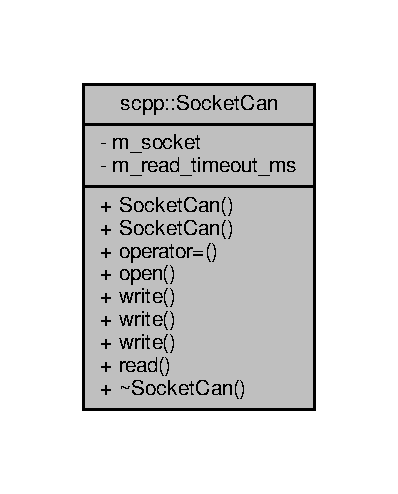
\includegraphics[width=191pt]{classscpp_1_1SocketCan__coll__graph}
\end{center}
\end{figure}
\subsection*{Public Member Functions}
\begin{DoxyCompactItemize}
\item 
\hyperlink{classscpp_1_1SocketCan_ac8947ab71c8ebf46f0bd0e7a3bd0e97a}{Socket\+Can} ()=default
\item 
\hyperlink{classscpp_1_1SocketCan_a837269bf5bc7edefb6ad17840ae3d867}{Socket\+Can} (const \hyperlink{classscpp_1_1SocketCan}{Socket\+Can} \&)=delete
\item 
\hyperlink{classscpp_1_1SocketCan}{Socket\+Can} \& \hyperlink{classscpp_1_1SocketCan_a474c925b2fb96b40a5cc549ba8134a44}{operator=} (const \hyperlink{classscpp_1_1SocketCan}{Socket\+Can} \&)=delete
\item 
\hyperlink{namespacescpp_abc60b9ed5f90c311397500d39ff15ef2}{Socket\+Can\+Status} \hyperlink{classscpp_1_1SocketCan_aa1ff7b90193c5beee33947a59c2e63bc}{open} (const char $\ast$can\+\_\+interface)
\item 
\hyperlink{namespacescpp_abc60b9ed5f90c311397500d39ff15ef2}{Socket\+Can\+Status} \hyperlink{classscpp_1_1SocketCan_af0e968a352380922dcde307e73b76f12}{write} (const uint8\+\_\+t $\ast$\+\_\+data, const uint32\+\_\+t \&\+\_\+id, const uint8\+\_\+t \&\+\_\+len)
\item 
\hyperlink{namespacescpp_abc60b9ed5f90c311397500d39ff15ef2}{Socket\+Can\+Status} \hyperlink{classscpp_1_1SocketCan_a323054409494c177ac8a5522d760c012}{write} (const \hyperlink{structscpp_1_1CanFrame}{Can\+Frame} \&msg)
\item 
\hyperlink{namespacescpp_abc60b9ed5f90c311397500d39ff15ef2}{Socket\+Can\+Status} \hyperlink{classscpp_1_1SocketCan_a3e4e4ca4931587c466801e01183942f4}{write} (struct canfd\+\_\+frame $\ast$frame)
\item 
\hyperlink{namespacescpp_abc60b9ed5f90c311397500d39ff15ef2}{Socket\+Can\+Status} \hyperlink{classscpp_1_1SocketCan_aa104c900d3e10722e3c1326c1322ee91}{read} (\hyperlink{structscpp_1_1CanFrame}{Can\+Frame} \&msg)
\item 
\hyperlink{classscpp_1_1SocketCan_abefe3a6fcbf0de1bf505d123eed9008e}{$\sim$\+Socket\+Can} ()
\end{DoxyCompactItemize}
\subsection*{Private Attributes}
\begin{DoxyCompactItemize}
\item 
int \hyperlink{classscpp_1_1SocketCan_a5a69eb3524f4dcc15bff5080934d60c8}{m\+\_\+socket} = -\/1
\item 
int32\+\_\+t \hyperlink{classscpp_1_1SocketCan_aa4d51fc60ada0d6ce29c112adedad63b}{m\+\_\+read\+\_\+timeout\+\_\+ms} = 3
\end{DoxyCompactItemize}


\subsection{Constructor \& Destructor Documentation}
\mbox{\Hypertarget{classscpp_1_1SocketCan_ac8947ab71c8ebf46f0bd0e7a3bd0e97a}\label{classscpp_1_1SocketCan_ac8947ab71c8ebf46f0bd0e7a3bd0e97a}} 
\index{scpp\+::\+Socket\+Can@{scpp\+::\+Socket\+Can}!Socket\+Can@{Socket\+Can}}
\index{Socket\+Can@{Socket\+Can}!scpp\+::\+Socket\+Can@{scpp\+::\+Socket\+Can}}
\subsubsection{\texorpdfstring{Socket\+Can()}{SocketCan()}\hspace{0.1cm}{\footnotesize\ttfamily [1/2]}}
{\footnotesize\ttfamily scpp\+::\+Socket\+Can\+::\+Socket\+Can (\begin{DoxyParamCaption}{ }\end{DoxyParamCaption})\hspace{0.3cm}{\ttfamily [default]}}

\mbox{\Hypertarget{classscpp_1_1SocketCan_a837269bf5bc7edefb6ad17840ae3d867}\label{classscpp_1_1SocketCan_a837269bf5bc7edefb6ad17840ae3d867}} 
\index{scpp\+::\+Socket\+Can@{scpp\+::\+Socket\+Can}!Socket\+Can@{Socket\+Can}}
\index{Socket\+Can@{Socket\+Can}!scpp\+::\+Socket\+Can@{scpp\+::\+Socket\+Can}}
\subsubsection{\texorpdfstring{Socket\+Can()}{SocketCan()}\hspace{0.1cm}{\footnotesize\ttfamily [2/2]}}
{\footnotesize\ttfamily scpp\+::\+Socket\+Can\+::\+Socket\+Can (\begin{DoxyParamCaption}\item[{const \hyperlink{classscpp_1_1SocketCan}{Socket\+Can} \&}]{ }\end{DoxyParamCaption})\hspace{0.3cm}{\ttfamily [delete]}}

\mbox{\Hypertarget{classscpp_1_1SocketCan_abefe3a6fcbf0de1bf505d123eed9008e}\label{classscpp_1_1SocketCan_abefe3a6fcbf0de1bf505d123eed9008e}} 
\index{scpp\+::\+Socket\+Can@{scpp\+::\+Socket\+Can}!````~Socket\+Can@{$\sim$\+Socket\+Can}}
\index{````~Socket\+Can@{$\sim$\+Socket\+Can}!scpp\+::\+Socket\+Can@{scpp\+::\+Socket\+Can}}
\subsubsection{\texorpdfstring{$\sim$\+Socket\+Can()}{~SocketCan()}}
{\footnotesize\ttfamily scpp\+::\+Socket\+Can\+::$\sim$\+Socket\+Can (\begin{DoxyParamCaption}{ }\end{DoxyParamCaption})}



\subsection{Member Function Documentation}
\mbox{\Hypertarget{classscpp_1_1SocketCan_aa1ff7b90193c5beee33947a59c2e63bc}\label{classscpp_1_1SocketCan_aa1ff7b90193c5beee33947a59c2e63bc}} 
\index{scpp\+::\+Socket\+Can@{scpp\+::\+Socket\+Can}!open@{open}}
\index{open@{open}!scpp\+::\+Socket\+Can@{scpp\+::\+Socket\+Can}}
\subsubsection{\texorpdfstring{open()}{open()}}
{\footnotesize\ttfamily \hyperlink{namespacescpp_abc60b9ed5f90c311397500d39ff15ef2}{Socket\+Can\+Status} scpp\+::\+Socket\+Can\+::open (\begin{DoxyParamCaption}\item[{const char $\ast$}]{can\+\_\+interface }\end{DoxyParamCaption})}

Here is the call graph for this function\+:
\nopagebreak
\begin{figure}[H]
\begin{center}
\leavevmode
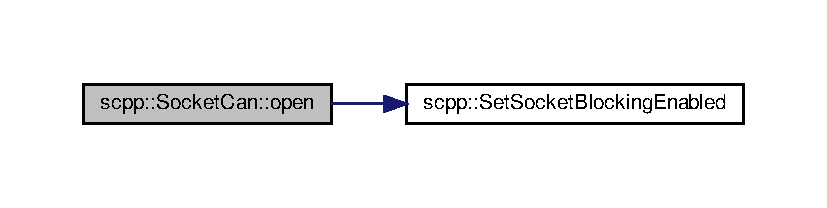
\includegraphics[width=350pt]{classscpp_1_1SocketCan_aa1ff7b90193c5beee33947a59c2e63bc_cgraph}
\end{center}
\end{figure}
Here is the caller graph for this function\+:
\nopagebreak
\begin{figure}[H]
\begin{center}
\leavevmode
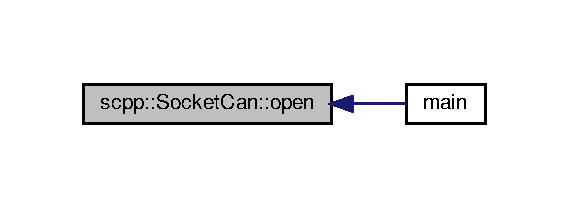
\includegraphics[width=273pt]{classscpp_1_1SocketCan_aa1ff7b90193c5beee33947a59c2e63bc_icgraph}
\end{center}
\end{figure}
\mbox{\Hypertarget{classscpp_1_1SocketCan_a474c925b2fb96b40a5cc549ba8134a44}\label{classscpp_1_1SocketCan_a474c925b2fb96b40a5cc549ba8134a44}} 
\index{scpp\+::\+Socket\+Can@{scpp\+::\+Socket\+Can}!operator=@{operator=}}
\index{operator=@{operator=}!scpp\+::\+Socket\+Can@{scpp\+::\+Socket\+Can}}
\subsubsection{\texorpdfstring{operator=()}{operator=()}}
{\footnotesize\ttfamily \hyperlink{classscpp_1_1SocketCan}{Socket\+Can}\& scpp\+::\+Socket\+Can\+::operator= (\begin{DoxyParamCaption}\item[{const \hyperlink{classscpp_1_1SocketCan}{Socket\+Can} \&}]{ }\end{DoxyParamCaption})\hspace{0.3cm}{\ttfamily [delete]}}

\mbox{\Hypertarget{classscpp_1_1SocketCan_aa104c900d3e10722e3c1326c1322ee91}\label{classscpp_1_1SocketCan_aa104c900d3e10722e3c1326c1322ee91}} 
\index{scpp\+::\+Socket\+Can@{scpp\+::\+Socket\+Can}!read@{read}}
\index{read@{read}!scpp\+::\+Socket\+Can@{scpp\+::\+Socket\+Can}}
\subsubsection{\texorpdfstring{read()}{read()}}
{\footnotesize\ttfamily \hyperlink{namespacescpp_abc60b9ed5f90c311397500d39ff15ef2}{Socket\+Can\+Status} scpp\+::\+Socket\+Can\+::read (\begin{DoxyParamCaption}\item[{\hyperlink{structscpp_1_1CanFrame}{Can\+Frame} \&}]{msg }\end{DoxyParamCaption})}

Here is the caller graph for this function\+:
\nopagebreak
\begin{figure}[H]
\begin{center}
\leavevmode
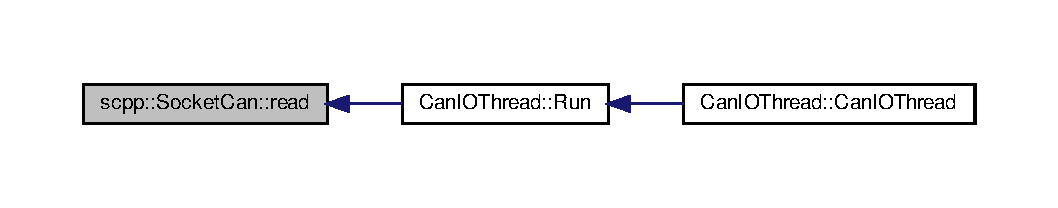
\includegraphics[width=350pt]{classscpp_1_1SocketCan_aa104c900d3e10722e3c1326c1322ee91_icgraph}
\end{center}
\end{figure}
\mbox{\Hypertarget{classscpp_1_1SocketCan_af0e968a352380922dcde307e73b76f12}\label{classscpp_1_1SocketCan_af0e968a352380922dcde307e73b76f12}} 
\index{scpp\+::\+Socket\+Can@{scpp\+::\+Socket\+Can}!write@{write}}
\index{write@{write}!scpp\+::\+Socket\+Can@{scpp\+::\+Socket\+Can}}
\subsubsection{\texorpdfstring{write()}{write()}\hspace{0.1cm}{\footnotesize\ttfamily [1/3]}}
{\footnotesize\ttfamily \hyperlink{namespacescpp_abc60b9ed5f90c311397500d39ff15ef2}{Socket\+Can\+Status} scpp\+::\+Socket\+Can\+::write (\begin{DoxyParamCaption}\item[{const uint8\+\_\+t $\ast$}]{\+\_\+data,  }\item[{const uint32\+\_\+t \&}]{\+\_\+id,  }\item[{const uint8\+\_\+t \&}]{\+\_\+len }\end{DoxyParamCaption})}

Here is the caller graph for this function\+:
\nopagebreak
\begin{figure}[H]
\begin{center}
\leavevmode
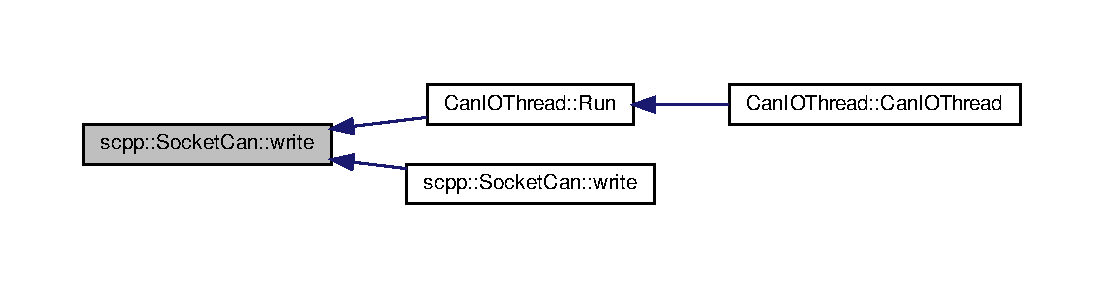
\includegraphics[width=350pt]{classscpp_1_1SocketCan_af0e968a352380922dcde307e73b76f12_icgraph}
\end{center}
\end{figure}
\mbox{\Hypertarget{classscpp_1_1SocketCan_a323054409494c177ac8a5522d760c012}\label{classscpp_1_1SocketCan_a323054409494c177ac8a5522d760c012}} 
\index{scpp\+::\+Socket\+Can@{scpp\+::\+Socket\+Can}!write@{write}}
\index{write@{write}!scpp\+::\+Socket\+Can@{scpp\+::\+Socket\+Can}}
\subsubsection{\texorpdfstring{write()}{write()}\hspace{0.1cm}{\footnotesize\ttfamily [2/3]}}
{\footnotesize\ttfamily \hyperlink{namespacescpp_abc60b9ed5f90c311397500d39ff15ef2}{Socket\+Can\+Status} scpp\+::\+Socket\+Can\+::write (\begin{DoxyParamCaption}\item[{const \hyperlink{structscpp_1_1CanFrame}{Can\+Frame} \&}]{msg }\end{DoxyParamCaption})}

Here is the call graph for this function\+:
\nopagebreak
\begin{figure}[H]
\begin{center}
\leavevmode
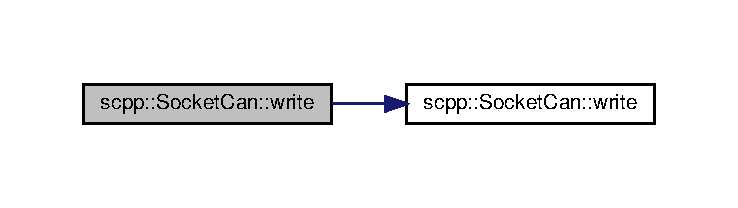
\includegraphics[width=350pt]{classscpp_1_1SocketCan_a323054409494c177ac8a5522d760c012_cgraph}
\end{center}
\end{figure}
\mbox{\Hypertarget{classscpp_1_1SocketCan_a3e4e4ca4931587c466801e01183942f4}\label{classscpp_1_1SocketCan_a3e4e4ca4931587c466801e01183942f4}} 
\index{scpp\+::\+Socket\+Can@{scpp\+::\+Socket\+Can}!write@{write}}
\index{write@{write}!scpp\+::\+Socket\+Can@{scpp\+::\+Socket\+Can}}
\subsubsection{\texorpdfstring{write()}{write()}\hspace{0.1cm}{\footnotesize\ttfamily [3/3]}}
{\footnotesize\ttfamily \hyperlink{namespacescpp_abc60b9ed5f90c311397500d39ff15ef2}{Socket\+Can\+Status} scpp\+::\+Socket\+Can\+::write (\begin{DoxyParamCaption}\item[{struct canfd\+\_\+frame $\ast$}]{frame }\end{DoxyParamCaption})}

Here is the call graph for this function\+:
\nopagebreak
\begin{figure}[H]
\begin{center}
\leavevmode
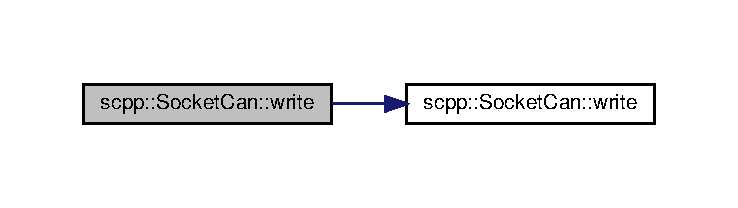
\includegraphics[width=350pt]{classscpp_1_1SocketCan_a3e4e4ca4931587c466801e01183942f4_cgraph}
\end{center}
\end{figure}


\subsection{Member Data Documentation}
\mbox{\Hypertarget{classscpp_1_1SocketCan_aa4d51fc60ada0d6ce29c112adedad63b}\label{classscpp_1_1SocketCan_aa4d51fc60ada0d6ce29c112adedad63b}} 
\index{scpp\+::\+Socket\+Can@{scpp\+::\+Socket\+Can}!m\+\_\+read\+\_\+timeout\+\_\+ms@{m\+\_\+read\+\_\+timeout\+\_\+ms}}
\index{m\+\_\+read\+\_\+timeout\+\_\+ms@{m\+\_\+read\+\_\+timeout\+\_\+ms}!scpp\+::\+Socket\+Can@{scpp\+::\+Socket\+Can}}
\subsubsection{\texorpdfstring{m\+\_\+read\+\_\+timeout\+\_\+ms}{m\_read\_timeout\_ms}}
{\footnotesize\ttfamily int32\+\_\+t scpp\+::\+Socket\+Can\+::m\+\_\+read\+\_\+timeout\+\_\+ms = 3\hspace{0.3cm}{\ttfamily [private]}}

\mbox{\Hypertarget{classscpp_1_1SocketCan_a5a69eb3524f4dcc15bff5080934d60c8}\label{classscpp_1_1SocketCan_a5a69eb3524f4dcc15bff5080934d60c8}} 
\index{scpp\+::\+Socket\+Can@{scpp\+::\+Socket\+Can}!m\+\_\+socket@{m\+\_\+socket}}
\index{m\+\_\+socket@{m\+\_\+socket}!scpp\+::\+Socket\+Can@{scpp\+::\+Socket\+Can}}
\subsubsection{\texorpdfstring{m\+\_\+socket}{m\_socket}}
{\footnotesize\ttfamily int scpp\+::\+Socket\+Can\+::m\+\_\+socket = -\/1\hspace{0.3cm}{\ttfamily [private]}}



The documentation for this class was generated from the following files\+:\begin{DoxyCompactItemize}
\item 
/home/rjohan59/repos/bootcamp\+\_\+course/project/source\+\_\+code/utils/include/\hyperlink{socketcan_8h}{socketcan.\+h}\item 
/home/rjohan59/repos/bootcamp\+\_\+course/project/source\+\_\+code/utils/src/\hyperlink{socketcan_8cpp}{socketcan.\+cpp}\end{DoxyCompactItemize}

\hypertarget{structuser__input__struct}{}\section{user\+\_\+input\+\_\+struct Struct Reference}
\label{structuser__input__struct}\index{user\+\_\+input\+\_\+struct@{user\+\_\+input\+\_\+struct}}


{\ttfamily \#include $<$user\+\_\+input.\+h$>$}



Collaboration diagram for user\+\_\+input\+\_\+struct\+:
\nopagebreak
\begin{figure}[H]
\begin{center}
\leavevmode
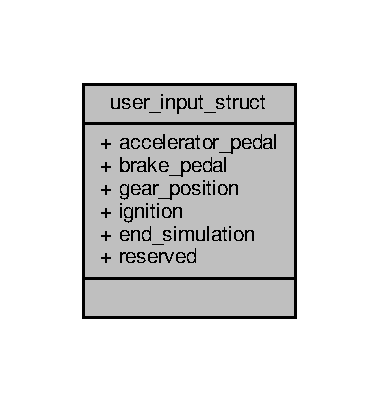
\includegraphics[width=182pt]{structuser__input__struct__coll__graph}
\end{center}
\end{figure}
\subsection*{Public Attributes}
\begin{DoxyCompactItemize}
\item 
uint8\+\_\+t \hyperlink{structuser__input__struct_a39c7303a5781506a884a8ddc6864f2df}{accelerator\+\_\+pedal}
\item 
uint8\+\_\+t \hyperlink{structuser__input__struct_a56ed67d835e5a9bde3de53c48fd1716e}{brake\+\_\+pedal}
\item 
uint8\+\_\+t \hyperlink{structuser__input__struct_ab8a73c513d97dc1278eff647a137bab4}{gear\+\_\+position}\+: 2
\item 
uint8\+\_\+t \hyperlink{structuser__input__struct_aea05665db1f1373882f6e149a1b6d6cd}{ignition}\+: 1
\item 
uint8\+\_\+t \hyperlink{structuser__input__struct_a3a25e9361a71de81d2f61e3c081388c3}{end\+\_\+simulation}\+: 1
\item 
uint8\+\_\+t \hyperlink{structuser__input__struct_af96dd6051734c0bba913919a208d3d13}{reserved}\+: 4
\end{DoxyCompactItemize}


\subsection{Member Data Documentation}
\mbox{\Hypertarget{structuser__input__struct_a39c7303a5781506a884a8ddc6864f2df}\label{structuser__input__struct_a39c7303a5781506a884a8ddc6864f2df}} 
\index{user\+\_\+input\+\_\+struct@{user\+\_\+input\+\_\+struct}!accelerator\+\_\+pedal@{accelerator\+\_\+pedal}}
\index{accelerator\+\_\+pedal@{accelerator\+\_\+pedal}!user\+\_\+input\+\_\+struct@{user\+\_\+input\+\_\+struct}}
\subsubsection{\texorpdfstring{accelerator\+\_\+pedal}{accelerator\_pedal}}
{\footnotesize\ttfamily uint8\+\_\+t user\+\_\+input\+\_\+struct\+::accelerator\+\_\+pedal}

\mbox{\Hypertarget{structuser__input__struct_a56ed67d835e5a9bde3de53c48fd1716e}\label{structuser__input__struct_a56ed67d835e5a9bde3de53c48fd1716e}} 
\index{user\+\_\+input\+\_\+struct@{user\+\_\+input\+\_\+struct}!brake\+\_\+pedal@{brake\+\_\+pedal}}
\index{brake\+\_\+pedal@{brake\+\_\+pedal}!user\+\_\+input\+\_\+struct@{user\+\_\+input\+\_\+struct}}
\subsubsection{\texorpdfstring{brake\+\_\+pedal}{brake\_pedal}}
{\footnotesize\ttfamily uint8\+\_\+t user\+\_\+input\+\_\+struct\+::brake\+\_\+pedal}

\mbox{\Hypertarget{structuser__input__struct_a3a25e9361a71de81d2f61e3c081388c3}\label{structuser__input__struct_a3a25e9361a71de81d2f61e3c081388c3}} 
\index{user\+\_\+input\+\_\+struct@{user\+\_\+input\+\_\+struct}!end\+\_\+simulation@{end\+\_\+simulation}}
\index{end\+\_\+simulation@{end\+\_\+simulation}!user\+\_\+input\+\_\+struct@{user\+\_\+input\+\_\+struct}}
\subsubsection{\texorpdfstring{end\+\_\+simulation}{end\_simulation}}
{\footnotesize\ttfamily uint8\+\_\+t user\+\_\+input\+\_\+struct\+::end\+\_\+simulation}

\mbox{\Hypertarget{structuser__input__struct_ab8a73c513d97dc1278eff647a137bab4}\label{structuser__input__struct_ab8a73c513d97dc1278eff647a137bab4}} 
\index{user\+\_\+input\+\_\+struct@{user\+\_\+input\+\_\+struct}!gear\+\_\+position@{gear\+\_\+position}}
\index{gear\+\_\+position@{gear\+\_\+position}!user\+\_\+input\+\_\+struct@{user\+\_\+input\+\_\+struct}}
\subsubsection{\texorpdfstring{gear\+\_\+position}{gear\_position}}
{\footnotesize\ttfamily uint8\+\_\+t user\+\_\+input\+\_\+struct\+::gear\+\_\+position}

\mbox{\Hypertarget{structuser__input__struct_aea05665db1f1373882f6e149a1b6d6cd}\label{structuser__input__struct_aea05665db1f1373882f6e149a1b6d6cd}} 
\index{user\+\_\+input\+\_\+struct@{user\+\_\+input\+\_\+struct}!ignition@{ignition}}
\index{ignition@{ignition}!user\+\_\+input\+\_\+struct@{user\+\_\+input\+\_\+struct}}
\subsubsection{\texorpdfstring{ignition}{ignition}}
{\footnotesize\ttfamily uint8\+\_\+t user\+\_\+input\+\_\+struct\+::ignition}

\mbox{\Hypertarget{structuser__input__struct_af96dd6051734c0bba913919a208d3d13}\label{structuser__input__struct_af96dd6051734c0bba913919a208d3d13}} 
\index{user\+\_\+input\+\_\+struct@{user\+\_\+input\+\_\+struct}!reserved@{reserved}}
\index{reserved@{reserved}!user\+\_\+input\+\_\+struct@{user\+\_\+input\+\_\+struct}}
\subsubsection{\texorpdfstring{reserved}{reserved}}
{\footnotesize\ttfamily uint8\+\_\+t user\+\_\+input\+\_\+struct\+::reserved}



The documentation for this struct was generated from the following file\+:\begin{DoxyCompactItemize}
\item 
/home/rjohan59/repos/bootcamp\+\_\+course/project/source\+\_\+code/utils/include/\hyperlink{user__input_8h}{user\+\_\+input.\+h}\end{DoxyCompactItemize}

\hypertarget{classVehicle}{}\section{Vehicle Class Reference}
\label{classVehicle}\index{Vehicle@{Vehicle}}


{\ttfamily \#include $<$vehicle.\+h$>$}



Collaboration diagram for Vehicle\+:
\nopagebreak
\begin{figure}[H]
\begin{center}
\leavevmode
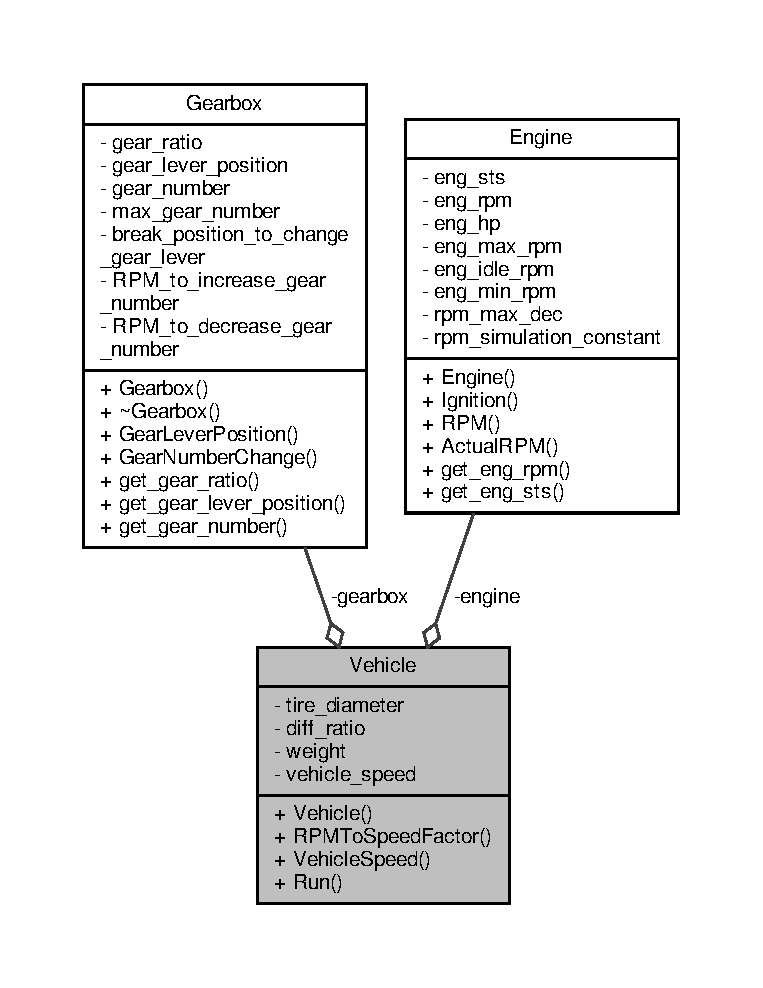
\includegraphics[width=350pt]{classVehicle__coll__graph}
\end{center}
\end{figure}
\subsection*{Public Member Functions}
\begin{DoxyCompactItemize}
\item 
\hyperlink{classVehicle_a545cb4416e5aa5c15311964a3de033fb}{Vehicle} (\hyperlink{classGearbox}{Gearbox} $\ast$\hyperlink{classVehicle_a5767df448358b995871f1caac195ea85}{gearbox}, \hyperlink{classEngine}{Engine} $\ast$\hyperlink{classVehicle_a84d681d0a67c864c023a84437d00ed21}{engine}, const float \&\hyperlink{classVehicle_ac24546ecc3efb25ea01e8d0e322c2785}{diff\+\_\+ratio}, const uint16\+\_\+t \&\hyperlink{classVehicle_aa7261c96ee3a5a4c039bf33432178fd9}{weight}, const float \&\hyperlink{classVehicle_ab36dab20fe34b27846ea5621693987f8}{tire\+\_\+diameter})
\item 
float \hyperlink{classVehicle_a52a12c60b5a8885dc9f95643c84958a8}{R\+P\+M\+To\+Speed\+Factor} ()
\item 
void \hyperlink{classVehicle_a0967229be7b0b40b3f84c86942e43a52}{Vehicle\+Speed} (const uint8\+\_\+t \&brk\+\_\+pedal, const float \&rpm\+\_\+to\+\_\+speed)
\item 
bool \hyperlink{classVehicle_a407e09d1ff69f43d3c4aa77f4f32a51c}{Run} ()
\end{DoxyCompactItemize}
\subsection*{Private Attributes}
\begin{DoxyCompactItemize}
\item 
\hyperlink{classEngine}{Engine} $\ast$ \hyperlink{classVehicle_a84d681d0a67c864c023a84437d00ed21}{engine}
\item 
\hyperlink{classGearbox}{Gearbox} $\ast$ \hyperlink{classVehicle_a5767df448358b995871f1caac195ea85}{gearbox}
\item 
float \hyperlink{classVehicle_ab36dab20fe34b27846ea5621693987f8}{tire\+\_\+diameter}
\item 
float \hyperlink{classVehicle_ac24546ecc3efb25ea01e8d0e322c2785}{diff\+\_\+ratio}
\item 
uint16\+\_\+t \hyperlink{classVehicle_aa7261c96ee3a5a4c039bf33432178fd9}{weight}
\item 
float \hyperlink{classVehicle_addeee407ebf67da1e69b608f6dda4656}{vehicle\+\_\+speed} =0
\end{DoxyCompactItemize}


\subsection{Constructor \& Destructor Documentation}
\mbox{\Hypertarget{classVehicle_a545cb4416e5aa5c15311964a3de033fb}\label{classVehicle_a545cb4416e5aa5c15311964a3de033fb}} 
\index{Vehicle@{Vehicle}!Vehicle@{Vehicle}}
\index{Vehicle@{Vehicle}!Vehicle@{Vehicle}}
\subsubsection{\texorpdfstring{Vehicle()}{Vehicle()}}
{\footnotesize\ttfamily Vehicle\+::\+Vehicle (\begin{DoxyParamCaption}\item[{\hyperlink{classGearbox}{Gearbox} $\ast$}]{gearbox,  }\item[{\hyperlink{classEngine}{Engine} $\ast$}]{engine,  }\item[{const float \&}]{diff\+\_\+ratio,  }\item[{const uint16\+\_\+t \&}]{weight,  }\item[{const float \&}]{tire\+\_\+diameter }\end{DoxyParamCaption})}

Constructor of \hyperlink{classVehicle}{Vehicle}. Assigns the class members. 
\begin{DoxyParams}{Parameters}
{\em gearbox} & gearbox simulation object \\
\hline
{\em engine} & engine simulation object \\
\hline
\end{DoxyParams}


\subsection{Member Function Documentation}
\mbox{\Hypertarget{classVehicle_a52a12c60b5a8885dc9f95643c84958a8}\label{classVehicle_a52a12c60b5a8885dc9f95643c84958a8}} 
\index{Vehicle@{Vehicle}!R\+P\+M\+To\+Speed\+Factor@{R\+P\+M\+To\+Speed\+Factor}}
\index{R\+P\+M\+To\+Speed\+Factor@{R\+P\+M\+To\+Speed\+Factor}!Vehicle@{Vehicle}}
\subsubsection{\texorpdfstring{R\+P\+M\+To\+Speed\+Factor()}{RPMToSpeedFactor()}}
{\footnotesize\ttfamily float Vehicle\+::\+R\+P\+M\+To\+Speed\+Factor (\begin{DoxyParamCaption}{ }\end{DoxyParamCaption})}

Function that calculates vehicle acceleration and speed 
\begin{DoxyParams}{Parameters}
{\em brake\+\_\+pedal} & brake pedal position \\
\hline
\end{DoxyParams}
\begin{DoxyReturn}{Returns}
calculated constant parapeter that can be used in the engine to 
\end{DoxyReturn}
Here is the call graph for this function\+:
\nopagebreak
\begin{figure}[H]
\begin{center}
\leavevmode
\includegraphics[width=350pt]{classVehicle_a52a12c60b5a8885dc9f95643c84958a8_cgraph}
\end{center}
\end{figure}
Here is the caller graph for this function\+:
\nopagebreak
\begin{figure}[H]
\begin{center}
\leavevmode
\includegraphics[width=350pt]{classVehicle_a52a12c60b5a8885dc9f95643c84958a8_icgraph}
\end{center}
\end{figure}
\mbox{\Hypertarget{classVehicle_a407e09d1ff69f43d3c4aa77f4f32a51c}\label{classVehicle_a407e09d1ff69f43d3c4aa77f4f32a51c}} 
\index{Vehicle@{Vehicle}!Run@{Run}}
\index{Run@{Run}!Vehicle@{Vehicle}}
\subsubsection{\texorpdfstring{Run()}{Run()}}
{\footnotesize\ttfamily bool Vehicle\+::\+Run (\begin{DoxyParamCaption}{ }\end{DoxyParamCaption})}

Pulls a C\+AN message from the receive buffer, checks the ID of the message and performs actions depending on the message. The output data will be put on the transmit buffer. Here is the call graph for this function\+:
\nopagebreak
\begin{figure}[H]
\begin{center}
\leavevmode
\includegraphics[width=350pt]{classVehicle_a407e09d1ff69f43d3c4aa77f4f32a51c_cgraph}
\end{center}
\end{figure}
Here is the caller graph for this function\+:
\nopagebreak
\begin{figure}[H]
\begin{center}
\leavevmode
\includegraphics[width=227pt]{classVehicle_a407e09d1ff69f43d3c4aa77f4f32a51c_icgraph}
\end{center}
\end{figure}
\mbox{\Hypertarget{classVehicle_a0967229be7b0b40b3f84c86942e43a52}\label{classVehicle_a0967229be7b0b40b3f84c86942e43a52}} 
\index{Vehicle@{Vehicle}!Vehicle\+Speed@{Vehicle\+Speed}}
\index{Vehicle\+Speed@{Vehicle\+Speed}!Vehicle@{Vehicle}}
\subsubsection{\texorpdfstring{Vehicle\+Speed()}{VehicleSpeed()}}
{\footnotesize\ttfamily void Vehicle\+::\+Vehicle\+Speed (\begin{DoxyParamCaption}\item[{const uint8\+\_\+t \&}]{brk\+\_\+pedal,  }\item[{const float \&}]{rpm\+\_\+to\+\_\+speed }\end{DoxyParamCaption})}

Here is the call graph for this function\+:
\nopagebreak
\begin{figure}[H]
\begin{center}
\leavevmode
\includegraphics[width=350pt]{classVehicle_a0967229be7b0b40b3f84c86942e43a52_cgraph}
\end{center}
\end{figure}
Here is the caller graph for this function\+:
\nopagebreak
\begin{figure}[H]
\begin{center}
\leavevmode
\includegraphics[width=350pt]{classVehicle_a0967229be7b0b40b3f84c86942e43a52_icgraph}
\end{center}
\end{figure}


\subsection{Member Data Documentation}
\mbox{\Hypertarget{classVehicle_ac24546ecc3efb25ea01e8d0e322c2785}\label{classVehicle_ac24546ecc3efb25ea01e8d0e322c2785}} 
\index{Vehicle@{Vehicle}!diff\+\_\+ratio@{diff\+\_\+ratio}}
\index{diff\+\_\+ratio@{diff\+\_\+ratio}!Vehicle@{Vehicle}}
\subsubsection{\texorpdfstring{diff\+\_\+ratio}{diff\_ratio}}
{\footnotesize\ttfamily float Vehicle\+::diff\+\_\+ratio\hspace{0.3cm}{\ttfamily [private]}}

\mbox{\Hypertarget{classVehicle_a84d681d0a67c864c023a84437d00ed21}\label{classVehicle_a84d681d0a67c864c023a84437d00ed21}} 
\index{Vehicle@{Vehicle}!engine@{engine}}
\index{engine@{engine}!Vehicle@{Vehicle}}
\subsubsection{\texorpdfstring{engine}{engine}}
{\footnotesize\ttfamily \hyperlink{classEngine}{Engine}$\ast$ Vehicle\+::engine\hspace{0.3cm}{\ttfamily [private]}}

\mbox{\Hypertarget{classVehicle_a5767df448358b995871f1caac195ea85}\label{classVehicle_a5767df448358b995871f1caac195ea85}} 
\index{Vehicle@{Vehicle}!gearbox@{gearbox}}
\index{gearbox@{gearbox}!Vehicle@{Vehicle}}
\subsubsection{\texorpdfstring{gearbox}{gearbox}}
{\footnotesize\ttfamily \hyperlink{classGearbox}{Gearbox}$\ast$ Vehicle\+::gearbox\hspace{0.3cm}{\ttfamily [private]}}

\mbox{\Hypertarget{classVehicle_ab36dab20fe34b27846ea5621693987f8}\label{classVehicle_ab36dab20fe34b27846ea5621693987f8}} 
\index{Vehicle@{Vehicle}!tire\+\_\+diameter@{tire\+\_\+diameter}}
\index{tire\+\_\+diameter@{tire\+\_\+diameter}!Vehicle@{Vehicle}}
\subsubsection{\texorpdfstring{tire\+\_\+diameter}{tire\_diameter}}
{\footnotesize\ttfamily float Vehicle\+::tire\+\_\+diameter\hspace{0.3cm}{\ttfamily [private]}}

\mbox{\Hypertarget{classVehicle_addeee407ebf67da1e69b608f6dda4656}\label{classVehicle_addeee407ebf67da1e69b608f6dda4656}} 
\index{Vehicle@{Vehicle}!vehicle\+\_\+speed@{vehicle\+\_\+speed}}
\index{vehicle\+\_\+speed@{vehicle\+\_\+speed}!Vehicle@{Vehicle}}
\subsubsection{\texorpdfstring{vehicle\+\_\+speed}{vehicle\_speed}}
{\footnotesize\ttfamily float Vehicle\+::vehicle\+\_\+speed =0\hspace{0.3cm}{\ttfamily [private]}}

\mbox{\Hypertarget{classVehicle_aa7261c96ee3a5a4c039bf33432178fd9}\label{classVehicle_aa7261c96ee3a5a4c039bf33432178fd9}} 
\index{Vehicle@{Vehicle}!weight@{weight}}
\index{weight@{weight}!Vehicle@{Vehicle}}
\subsubsection{\texorpdfstring{weight}{weight}}
{\footnotesize\ttfamily uint16\+\_\+t Vehicle\+::weight\hspace{0.3cm}{\ttfamily [private]}}



The documentation for this class was generated from the following files\+:\begin{DoxyCompactItemize}
\item 
/home/rjohan59/repos/bootcamp\+\_\+course/project/source\+\_\+code/drivetrain/include/\hyperlink{vehicle_8h}{vehicle.\+h}\item 
/home/rjohan59/repos/bootcamp\+\_\+course/project/source\+\_\+code/drivetrain/src/\hyperlink{vehicle_8cpp}{vehicle.\+cpp}\end{DoxyCompactItemize}

\chapter{File Documentation}
\hypertarget{engine__simulator_8h}{}\section{/home/rjohan59/repos/bootcamp\+\_\+course/project/source\+\_\+code/drivetrain/include/engine\+\_\+simulator.h File Reference}
\label{engine__simulator_8h}\index{/home/rjohan59/repos/bootcamp\+\_\+course/project/source\+\_\+code/drivetrain/include/engine\+\_\+simulator.\+h@{/home/rjohan59/repos/bootcamp\+\_\+course/project/source\+\_\+code/drivetrain/include/engine\+\_\+simulator.\+h}}
{\ttfamily \#include \char`\"{}user\+\_\+input.\+h\char`\"{}}\newline
{\ttfamily \#include $<$math.\+h$>$}\newline
Include dependency graph for engine\+\_\+simulator.\+h\+:
\nopagebreak
\begin{figure}[H]
\begin{center}
\leavevmode
\includegraphics[width=240pt]{engine__simulator_8h__incl}
\end{center}
\end{figure}
This graph shows which files directly or indirectly include this file\+:
\nopagebreak
\begin{figure}[H]
\begin{center}
\leavevmode
\includegraphics[width=350pt]{engine__simulator_8h__dep__incl}
\end{center}
\end{figure}
\subsection*{Classes}
\begin{DoxyCompactItemize}
\item 
class \hyperlink{classEngine}{Engine}
\end{DoxyCompactItemize}
\subsection*{Enumerations}
\begin{DoxyCompactItemize}
\item 
enum \hyperlink{engine__simulator_8h_a66f867cac759503312677c598e4d30f5}{Eng\+Sts} \+: uint8\+\_\+t \{ \hyperlink{engine__simulator_8h_a66f867cac759503312677c598e4d30f5ad8a892b94d3a94ea861543c085ae782b}{Off} = 0, 
\hyperlink{engine__simulator_8h_a66f867cac759503312677c598e4d30f5ad86d047cb88457a513e7287560fb2b31}{On} = 1
 \}
\end{DoxyCompactItemize}


\subsection{Enumeration Type Documentation}
\mbox{\Hypertarget{engine__simulator_8h_a66f867cac759503312677c598e4d30f5}\label{engine__simulator_8h_a66f867cac759503312677c598e4d30f5}} 
\index{engine\+\_\+simulator.\+h@{engine\+\_\+simulator.\+h}!Eng\+Sts@{Eng\+Sts}}
\index{Eng\+Sts@{Eng\+Sts}!engine\+\_\+simulator.\+h@{engine\+\_\+simulator.\+h}}
\subsubsection{\texorpdfstring{Eng\+Sts}{EngSts}}
{\footnotesize\ttfamily enum \hyperlink{engine__simulator_8h_a66f867cac759503312677c598e4d30f5}{Eng\+Sts} \+: uint8\+\_\+t}

\begin{DoxyEnumFields}{Enumerator}
\raisebox{\heightof{T}}[0pt][0pt]{\index{Off@{Off}!engine\+\_\+simulator.\+h@{engine\+\_\+simulator.\+h}}\index{engine\+\_\+simulator.\+h@{engine\+\_\+simulator.\+h}!Off@{Off}}}\mbox{\Hypertarget{engine__simulator_8h_a66f867cac759503312677c598e4d30f5ad8a892b94d3a94ea861543c085ae782b}\label{engine__simulator_8h_a66f867cac759503312677c598e4d30f5ad8a892b94d3a94ea861543c085ae782b}} 
Off&\\
\hline

\raisebox{\heightof{T}}[0pt][0pt]{\index{On@{On}!engine\+\_\+simulator.\+h@{engine\+\_\+simulator.\+h}}\index{engine\+\_\+simulator.\+h@{engine\+\_\+simulator.\+h}!On@{On}}}\mbox{\Hypertarget{engine__simulator_8h_a66f867cac759503312677c598e4d30f5ad86d047cb88457a513e7287560fb2b31}\label{engine__simulator_8h_a66f867cac759503312677c598e4d30f5ad86d047cb88457a513e7287560fb2b31}} 
On&\\
\hline

\end{DoxyEnumFields}

\hypertarget{gearbox__simulator_8h}{}\section{/home/rjohan59/repos/bootcamp\+\_\+course/project/source\+\_\+code/drivetrain/include/gearbox\+\_\+simulator.h File Reference}
\label{gearbox__simulator_8h}\index{/home/rjohan59/repos/bootcamp\+\_\+course/project/source\+\_\+code/drivetrain/include/gearbox\+\_\+simulator.\+h@{/home/rjohan59/repos/bootcamp\+\_\+course/project/source\+\_\+code/drivetrain/include/gearbox\+\_\+simulator.\+h}}
{\ttfamily \#include \char`\"{}user\+\_\+input.\+h\char`\"{}}\newline
Include dependency graph for gearbox\+\_\+simulator.\+h\+:
\nopagebreak
\begin{figure}[H]
\begin{center}
\leavevmode
\includegraphics[width=221pt]{gearbox__simulator_8h__incl}
\end{center}
\end{figure}
This graph shows which files directly or indirectly include this file\+:
\nopagebreak
\begin{figure}[H]
\begin{center}
\leavevmode
\includegraphics[width=350pt]{gearbox__simulator_8h__dep__incl}
\end{center}
\end{figure}
\subsection*{Classes}
\begin{DoxyCompactItemize}
\item 
class \hyperlink{classGearbox}{Gearbox}
\end{DoxyCompactItemize}

\hypertarget{ringbuffer_8h}{}\section{/home/rjohan59/repos/bootcamp\+\_\+course/project/source\+\_\+code/drivetrain/include/ringbuffer.h File Reference}
\label{ringbuffer_8h}\index{/home/rjohan59/repos/bootcamp\+\_\+course/project/source\+\_\+code/drivetrain/include/ringbuffer.\+h@{/home/rjohan59/repos/bootcamp\+\_\+course/project/source\+\_\+code/drivetrain/include/ringbuffer.\+h}}
{\ttfamily \#include $<$iostream$>$}\newline
Include dependency graph for ringbuffer.\+h\+:
\nopagebreak
\begin{figure}[H]
\begin{center}
\leavevmode
\includegraphics[width=209pt]{ringbuffer_8h__incl}
\end{center}
\end{figure}
\subsection*{Classes}
\begin{DoxyCompactItemize}
\item 
class \hyperlink{classRingbuffer}{Ringbuffer$<$ T, size $>$}
\end{DoxyCompactItemize}

\hypertarget{vehicle_8h}{}\section{/home/rjohan59/repos/bootcamp\+\_\+course/project/source\+\_\+code/drivetrain/include/vehicle.h File Reference}
\label{vehicle_8h}\index{/home/rjohan59/repos/bootcamp\+\_\+course/project/source\+\_\+code/drivetrain/include/vehicle.\+h@{/home/rjohan59/repos/bootcamp\+\_\+course/project/source\+\_\+code/drivetrain/include/vehicle.\+h}}
{\ttfamily \#include \char`\"{}engine\+\_\+simulator.\+h\char`\"{}}\newline
{\ttfamily \#include \char`\"{}gearbox\+\_\+simulator.\+h\char`\"{}}\newline
{\ttfamily \#include \char`\"{}user\+\_\+input.\+h\char`\"{}}\newline
{\ttfamily \#include \char`\"{}can\+\_\+buffer.\+h\char`\"{}}\newline
{\ttfamily \#include $<$thread$>$}\newline
Include dependency graph for vehicle.\+h\+:
\nopagebreak
\begin{figure}[H]
\begin{center}
\leavevmode
\includegraphics[width=350pt]{vehicle_8h__incl}
\end{center}
\end{figure}
This graph shows which files directly or indirectly include this file\+:
\nopagebreak
\begin{figure}[H]
\begin{center}
\leavevmode
\includegraphics[width=350pt]{vehicle_8h__dep__incl}
\end{center}
\end{figure}
\subsection*{Classes}
\begin{DoxyCompactItemize}
\item 
class \hyperlink{classVehicle}{Vehicle}
\end{DoxyCompactItemize}
\subsection*{Variables}
\begin{DoxyCompactItemize}
\item 
const uint32\+\_\+t \hyperlink{vehicle_8h_a7abcdb7b42f0351950ab18e61491d868}{transmit\+\_\+id} = 2
\item 
const uint8\+\_\+t \hyperlink{vehicle_8h_a551ca3bad83664aca3aeb8284f552c67}{transmit\+\_\+length} = 5
\item 
const uint16\+\_\+t \hyperlink{vehicle_8h_ad03a4c966aec416c3a2461f6136eeee3}{sampletime\+\_\+micro} = 5
\end{DoxyCompactItemize}


\subsection{Variable Documentation}
\mbox{\Hypertarget{vehicle_8h_ad03a4c966aec416c3a2461f6136eeee3}\label{vehicle_8h_ad03a4c966aec416c3a2461f6136eeee3}} 
\index{vehicle.\+h@{vehicle.\+h}!sampletime\+\_\+micro@{sampletime\+\_\+micro}}
\index{sampletime\+\_\+micro@{sampletime\+\_\+micro}!vehicle.\+h@{vehicle.\+h}}
\subsubsection{\texorpdfstring{sampletime\+\_\+micro}{sampletime\_micro}}
{\footnotesize\ttfamily const uint16\+\_\+t sampletime\+\_\+micro = 5}

\mbox{\Hypertarget{vehicle_8h_a7abcdb7b42f0351950ab18e61491d868}\label{vehicle_8h_a7abcdb7b42f0351950ab18e61491d868}} 
\index{vehicle.\+h@{vehicle.\+h}!transmit\+\_\+id@{transmit\+\_\+id}}
\index{transmit\+\_\+id@{transmit\+\_\+id}!vehicle.\+h@{vehicle.\+h}}
\subsubsection{\texorpdfstring{transmit\+\_\+id}{transmit\_id}}
{\footnotesize\ttfamily const uint32\+\_\+t transmit\+\_\+id = 2}

\mbox{\Hypertarget{vehicle_8h_a551ca3bad83664aca3aeb8284f552c67}\label{vehicle_8h_a551ca3bad83664aca3aeb8284f552c67}} 
\index{vehicle.\+h@{vehicle.\+h}!transmit\+\_\+length@{transmit\+\_\+length}}
\index{transmit\+\_\+length@{transmit\+\_\+length}!vehicle.\+h@{vehicle.\+h}}
\subsubsection{\texorpdfstring{transmit\+\_\+length}{transmit\_length}}
{\footnotesize\ttfamily const uint8\+\_\+t transmit\+\_\+length = 5}


\hypertarget{engine__simulator_8cpp}{}\section{/home/rjohan59/repos/bootcamp\+\_\+course/project/source\+\_\+code/drivetrain/src/engine\+\_\+simulator.cpp File Reference}
\label{engine__simulator_8cpp}\index{/home/rjohan59/repos/bootcamp\+\_\+course/project/source\+\_\+code/drivetrain/src/engine\+\_\+simulator.\+cpp@{/home/rjohan59/repos/bootcamp\+\_\+course/project/source\+\_\+code/drivetrain/src/engine\+\_\+simulator.\+cpp}}
{\ttfamily \#include $<$iostream$>$}\newline
{\ttfamily \#include \char`\"{}engine\+\_\+simulator.\+h\char`\"{}}\newline
{\ttfamily \#include \char`\"{}user\+\_\+input.\+h\char`\"{}}\newline
Include dependency graph for engine\+\_\+simulator.\+cpp\+:
\nopagebreak
\begin{figure}[H]
\begin{center}
\leavevmode
\includegraphics[width=288pt]{engine__simulator_8cpp__incl}
\end{center}
\end{figure}

\hypertarget{gearbox__simulator_8cpp}{}\section{/home/rjohan59/repos/bootcamp\+\_\+course/project/source\+\_\+code/drivetrain/src/gearbox\+\_\+simulator.cpp File Reference}
\label{gearbox__simulator_8cpp}\index{/home/rjohan59/repos/bootcamp\+\_\+course/project/source\+\_\+code/drivetrain/src/gearbox\+\_\+simulator.\+cpp@{/home/rjohan59/repos/bootcamp\+\_\+course/project/source\+\_\+code/drivetrain/src/gearbox\+\_\+simulator.\+cpp}}
{\ttfamily \#include \char`\"{}gearbox\+\_\+simulator.\+h\char`\"{}}\newline
Include dependency graph for gearbox\+\_\+simulator.\+cpp\+:
\nopagebreak
\begin{figure}[H]
\begin{center}
\leavevmode
\includegraphics[width=214pt]{gearbox__simulator_8cpp__incl}
\end{center}
\end{figure}

\hypertarget{drivetrain_2src_2main_8cpp}{}\section{/home/rjohan59/repos/bootcamp\+\_\+course/project/source\+\_\+code/drivetrain/src/main.cpp File Reference}
\label{drivetrain_2src_2main_8cpp}\index{/home/rjohan59/repos/bootcamp\+\_\+course/project/source\+\_\+code/drivetrain/src/main.\+cpp@{/home/rjohan59/repos/bootcamp\+\_\+course/project/source\+\_\+code/drivetrain/src/main.\+cpp}}
{\ttfamily \#include \char`\"{}vehicle.\+h\char`\"{}}\newline
{\ttfamily \#include \char`\"{}can\+\_\+io\+\_\+thread.\+h\char`\"{}}\newline
{\ttfamily \#include $<$iostream$>$}\newline
Include dependency graph for main.\+cpp\+:
\nopagebreak
\begin{figure}[H]
\begin{center}
\leavevmode
\includegraphics[width=350pt]{drivetrain_2src_2main_8cpp__incl}
\end{center}
\end{figure}
\subsection*{Functions}
\begin{DoxyCompactItemize}
\item 
int \hyperlink{drivetrain_2src_2main_8cpp_ae66f6b31b5ad750f1fe042a706a4e3d4}{main} ()
\end{DoxyCompactItemize}
\subsection*{Variables}
\begin{DoxyCompactItemize}
\item 
const float \hyperlink{drivetrain_2src_2main_8cpp_a3cb00d54bc228826aa4ab337278e45f1}{final\+\_\+gear} = 3.\+42
\item 
const float \hyperlink{drivetrain_2src_2main_8cpp_a5cfb00cce30511af424fbaef1e7c453d}{weight} = 1000
\item 
const float \hyperlink{drivetrain_2src_2main_8cpp_a984b3b132fccfa1fc4d70a9cd64de55c}{tire\+\_\+diameter} = 0.\+680
\end{DoxyCompactItemize}


\subsection{Function Documentation}
\mbox{\Hypertarget{drivetrain_2src_2main_8cpp_ae66f6b31b5ad750f1fe042a706a4e3d4}\label{drivetrain_2src_2main_8cpp_ae66f6b31b5ad750f1fe042a706a4e3d4}} 
\index{drivetrain/src/main.\+cpp@{drivetrain/src/main.\+cpp}!main@{main}}
\index{main@{main}!drivetrain/src/main.\+cpp@{drivetrain/src/main.\+cpp}}
\subsubsection{\texorpdfstring{main()}{main()}}
{\footnotesize\ttfamily int main (\begin{DoxyParamCaption}{ }\end{DoxyParamCaption})}

Here is the call graph for this function\+:
\nopagebreak
\begin{figure}[H]
\begin{center}
\leavevmode
\includegraphics[width=350pt]{drivetrain_2src_2main_8cpp_ae66f6b31b5ad750f1fe042a706a4e3d4_cgraph}
\end{center}
\end{figure}


\subsection{Variable Documentation}
\mbox{\Hypertarget{drivetrain_2src_2main_8cpp_a3cb00d54bc228826aa4ab337278e45f1}\label{drivetrain_2src_2main_8cpp_a3cb00d54bc228826aa4ab337278e45f1}} 
\index{drivetrain/src/main.\+cpp@{drivetrain/src/main.\+cpp}!final\+\_\+gear@{final\+\_\+gear}}
\index{final\+\_\+gear@{final\+\_\+gear}!drivetrain/src/main.\+cpp@{drivetrain/src/main.\+cpp}}
\subsubsection{\texorpdfstring{final\+\_\+gear}{final\_gear}}
{\footnotesize\ttfamily const float final\+\_\+gear = 3.\+42}

\mbox{\Hypertarget{drivetrain_2src_2main_8cpp_a984b3b132fccfa1fc4d70a9cd64de55c}\label{drivetrain_2src_2main_8cpp_a984b3b132fccfa1fc4d70a9cd64de55c}} 
\index{drivetrain/src/main.\+cpp@{drivetrain/src/main.\+cpp}!tire\+\_\+diameter@{tire\+\_\+diameter}}
\index{tire\+\_\+diameter@{tire\+\_\+diameter}!drivetrain/src/main.\+cpp@{drivetrain/src/main.\+cpp}}
\subsubsection{\texorpdfstring{tire\+\_\+diameter}{tire\_diameter}}
{\footnotesize\ttfamily const float tire\+\_\+diameter = 0.\+680}

\mbox{\Hypertarget{drivetrain_2src_2main_8cpp_a5cfb00cce30511af424fbaef1e7c453d}\label{drivetrain_2src_2main_8cpp_a5cfb00cce30511af424fbaef1e7c453d}} 
\index{drivetrain/src/main.\+cpp@{drivetrain/src/main.\+cpp}!weight@{weight}}
\index{weight@{weight}!drivetrain/src/main.\+cpp@{drivetrain/src/main.\+cpp}}
\subsubsection{\texorpdfstring{weight}{weight}}
{\footnotesize\ttfamily const float weight = 1000}


\hypertarget{input__handler_2src_2main_8cpp}{}\section{/home/rjohan59/repos/bootcamp\+\_\+course/project/source\+\_\+code/input\+\_\+handler/src/main.cpp File Reference}
\label{input__handler_2src_2main_8cpp}\index{/home/rjohan59/repos/bootcamp\+\_\+course/project/source\+\_\+code/input\+\_\+handler/src/main.\+cpp@{/home/rjohan59/repos/bootcamp\+\_\+course/project/source\+\_\+code/input\+\_\+handler/src/main.\+cpp}}
{\ttfamily \#include $<$thread$>$}\newline
{\ttfamily \#include $<$chrono$>$}\newline
{\ttfamily \#include $<$mutex$>$}\newline
{\ttfamily \#include $<$iostream$>$}\newline
{\ttfamily \#include $<$future$>$}\newline
{\ttfamily \#include $<$cstring$>$}\newline
{\ttfamily \#include \char`\"{}keyboard\+\_\+input\+\_\+reader.\+h\char`\"{}}\newline
{\ttfamily \#include \char`\"{}can\+\_\+io\+\_\+thread.\+h\char`\"{}}\newline
{\ttfamily \#include \char`\"{}can\+\_\+buffer.\+h\char`\"{}}\newline
Include dependency graph for main.\+cpp\+:
\nopagebreak
\begin{figure}[H]
\begin{center}
\leavevmode
\includegraphics[width=350pt]{input__handler_2src_2main_8cpp__incl}
\end{center}
\end{figure}
\subsection*{Functions}
\begin{DoxyCompactItemize}
\item 
int \hyperlink{input__handler_2src_2main_8cpp_ae66f6b31b5ad750f1fe042a706a4e3d4}{main} ()
\end{DoxyCompactItemize}


\subsection{Function Documentation}
\mbox{\Hypertarget{input__handler_2src_2main_8cpp_ae66f6b31b5ad750f1fe042a706a4e3d4}\label{input__handler_2src_2main_8cpp_ae66f6b31b5ad750f1fe042a706a4e3d4}} 
\index{input\+\_\+handler/src/main.\+cpp@{input\+\_\+handler/src/main.\+cpp}!main@{main}}
\index{main@{main}!input\+\_\+handler/src/main.\+cpp@{input\+\_\+handler/src/main.\+cpp}}
\subsubsection{\texorpdfstring{main()}{main()}}
{\footnotesize\ttfamily int main (\begin{DoxyParamCaption}{ }\end{DoxyParamCaption})}

Here is the call graph for this function\+:
\nopagebreak
\begin{figure}[H]
\begin{center}
\leavevmode
\includegraphics[width=350pt]{input__handler_2src_2main_8cpp_ae66f6b31b5ad750f1fe042a706a4e3d4_cgraph}
\end{center}
\end{figure}

\hypertarget{output__handler_2src_2main_8cpp}{}\section{/home/rjohan59/repos/bootcamp\+\_\+course/project/source\+\_\+code/output\+\_\+handler/src/main.cpp File Reference}
\label{output__handler_2src_2main_8cpp}\index{/home/rjohan59/repos/bootcamp\+\_\+course/project/source\+\_\+code/output\+\_\+handler/src/main.\+cpp@{/home/rjohan59/repos/bootcamp\+\_\+course/project/source\+\_\+code/output\+\_\+handler/src/main.\+cpp}}
{\ttfamily \#include $<$thread$>$}\newline
{\ttfamily \#include \char`\"{}can\+\_\+io\+\_\+thread.\+h\char`\"{}}\newline
{\ttfamily \#include $<$chrono$>$}\newline
{\ttfamily \#include $<$iostream$>$}\newline
{\ttfamily \#include \char`\"{}socketcan.\+h\char`\"{}}\newline
Include dependency graph for main.\+cpp\+:
\nopagebreak
\begin{figure}[H]
\begin{center}
\leavevmode
\includegraphics[width=350pt]{output__handler_2src_2main_8cpp__incl}
\end{center}
\end{figure}
\subsection*{Functions}
\begin{DoxyCompactItemize}
\item 
int \hyperlink{output__handler_2src_2main_8cpp_ae66f6b31b5ad750f1fe042a706a4e3d4}{main} ()
\end{DoxyCompactItemize}


\subsection{Function Documentation}
\mbox{\Hypertarget{output__handler_2src_2main_8cpp_ae66f6b31b5ad750f1fe042a706a4e3d4}\label{output__handler_2src_2main_8cpp_ae66f6b31b5ad750f1fe042a706a4e3d4}} 
\index{output\+\_\+handler/src/main.\+cpp@{output\+\_\+handler/src/main.\+cpp}!main@{main}}
\index{main@{main}!output\+\_\+handler/src/main.\+cpp@{output\+\_\+handler/src/main.\+cpp}}
\subsubsection{\texorpdfstring{main()}{main()}}
{\footnotesize\ttfamily int main (\begin{DoxyParamCaption}{ }\end{DoxyParamCaption})}

Here is the call graph for this function\+:
\nopagebreak
\begin{figure}[H]
\begin{center}
\leavevmode
\includegraphics[width=350pt]{output__handler_2src_2main_8cpp_ae66f6b31b5ad750f1fe042a706a4e3d4_cgraph}
\end{center}
\end{figure}

\hypertarget{vehicle_8cpp}{}\section{/home/rjohan59/repos/bootcamp\+\_\+course/project/source\+\_\+code/drivetrain/src/vehicle.cpp File Reference}
\label{vehicle_8cpp}\index{/home/rjohan59/repos/bootcamp\+\_\+course/project/source\+\_\+code/drivetrain/src/vehicle.\+cpp@{/home/rjohan59/repos/bootcamp\+\_\+course/project/source\+\_\+code/drivetrain/src/vehicle.\+cpp}}
{\ttfamily \#include \char`\"{}vehicle.\+h\char`\"{}}\newline
{\ttfamily \#include $<$iostream$>$}\newline
{\ttfamily \#include $<$math.\+h$>$}\newline
Include dependency graph for vehicle.\+cpp\+:
\nopagebreak
\begin{figure}[H]
\begin{center}
\leavevmode
\includegraphics[width=350pt]{vehicle_8cpp__incl}
\end{center}
\end{figure}
\subsection*{Functions}
\begin{DoxyCompactItemize}
\item 
float \hyperlink{vehicle_8cpp_a6597511c111033c86174e181164d1fdd}{calculate\+\_\+resistance} (uint16\+\_\+t \hyperlink{drivetrain_2src_2main_8cpp_a5cfb00cce30511af424fbaef1e7c453d}{weight}, float speed)
\item 
float \hyperlink{vehicle_8cpp_abbcf47b233d59122a5451591b6b6bebf}{calculate\+\_\+engine\+\_\+tq} (uint16\+\_\+t engine\+\_\+speed)
\item 
float \hyperlink{vehicle_8cpp_aa3ffa21149a5a339a380677de0e5d594}{calculate\+\_\+brake\+\_\+tq} (uint8\+\_\+t brake\+\_\+pedal)
\end{DoxyCompactItemize}


\subsection{Function Documentation}
\mbox{\Hypertarget{vehicle_8cpp_aa3ffa21149a5a339a380677de0e5d594}\label{vehicle_8cpp_aa3ffa21149a5a339a380677de0e5d594}} 
\index{vehicle.\+cpp@{vehicle.\+cpp}!calculate\+\_\+brake\+\_\+tq@{calculate\+\_\+brake\+\_\+tq}}
\index{calculate\+\_\+brake\+\_\+tq@{calculate\+\_\+brake\+\_\+tq}!vehicle.\+cpp@{vehicle.\+cpp}}
\subsubsection{\texorpdfstring{calculate\+\_\+brake\+\_\+tq()}{calculate\_brake\_tq()}}
{\footnotesize\ttfamily float calculate\+\_\+brake\+\_\+tq (\begin{DoxyParamCaption}\item[{uint8\+\_\+t}]{brake\+\_\+pedal }\end{DoxyParamCaption})}

Function that mimics brake pedal action might require calibration 
\begin{DoxyParams}{Parameters}
{\em brake\+\_\+pedal} & brake pedal position \\
\hline
\end{DoxyParams}
\begin{DoxyReturn}{Returns}
calculated brake force 
\end{DoxyReturn}
Here is the caller graph for this function\+:
\nopagebreak
\begin{figure}[H]
\begin{center}
\leavevmode
\includegraphics[width=350pt]{vehicle_8cpp_aa3ffa21149a5a339a380677de0e5d594_icgraph}
\end{center}
\end{figure}
\mbox{\Hypertarget{vehicle_8cpp_abbcf47b233d59122a5451591b6b6bebf}\label{vehicle_8cpp_abbcf47b233d59122a5451591b6b6bebf}} 
\index{vehicle.\+cpp@{vehicle.\+cpp}!calculate\+\_\+engine\+\_\+tq@{calculate\+\_\+engine\+\_\+tq}}
\index{calculate\+\_\+engine\+\_\+tq@{calculate\+\_\+engine\+\_\+tq}!vehicle.\+cpp@{vehicle.\+cpp}}
\subsubsection{\texorpdfstring{calculate\+\_\+engine\+\_\+tq()}{calculate\_engine\_tq()}}
{\footnotesize\ttfamily float calculate\+\_\+engine\+\_\+tq (\begin{DoxyParamCaption}\item[{uint16\+\_\+t}]{engine\+\_\+speed }\end{DoxyParamCaption})}

Function used to compute engine torque dependent on engine rpm, should be okey without calibraion 
\begin{DoxyParams}{Parameters}
{\em engine\+\_\+speed} & R\+PM of the engine \\
\hline
\end{DoxyParams}
\begin{DoxyReturn}{Returns}
calculated engine torqe 
\end{DoxyReturn}
\mbox{\Hypertarget{vehicle_8cpp_a6597511c111033c86174e181164d1fdd}\label{vehicle_8cpp_a6597511c111033c86174e181164d1fdd}} 
\index{vehicle.\+cpp@{vehicle.\+cpp}!calculate\+\_\+resistance@{calculate\+\_\+resistance}}
\index{calculate\+\_\+resistance@{calculate\+\_\+resistance}!vehicle.\+cpp@{vehicle.\+cpp}}
\subsubsection{\texorpdfstring{calculate\+\_\+resistance()}{calculate\_resistance()}}
{\footnotesize\ttfamily float calculate\+\_\+resistance (\begin{DoxyParamCaption}\item[{uint16\+\_\+t}]{weight,  }\item[{float}]{speed }\end{DoxyParamCaption})}

Function used to calculate vehicle rolling resistance depending on veh speed, needs calibration possibly 
\begin{DoxyParams}{Parameters}
{\em weight} & vehicle weight \\
\hline
{\em speed} & speed of the vehicle \\
\hline
\end{DoxyParams}
\begin{DoxyReturn}{Returns}
calculated rolling resistance 
\end{DoxyReturn}
Here is the caller graph for this function\+:
\nopagebreak
\begin{figure}[H]
\begin{center}
\leavevmode
\includegraphics[width=350pt]{vehicle_8cpp_a6597511c111033c86174e181164d1fdd_icgraph}
\end{center}
\end{figure}

\hypertarget{keyboard__input__reader_8h}{}\section{/home/rjohan59/repos/bootcamp\+\_\+course/project/source\+\_\+code/input\+\_\+handler/include/keyboard\+\_\+input\+\_\+reader.h File Reference}
\label{keyboard__input__reader_8h}\index{/home/rjohan59/repos/bootcamp\+\_\+course/project/source\+\_\+code/input\+\_\+handler/include/keyboard\+\_\+input\+\_\+reader.\+h@{/home/rjohan59/repos/bootcamp\+\_\+course/project/source\+\_\+code/input\+\_\+handler/include/keyboard\+\_\+input\+\_\+reader.\+h}}
{\ttfamily \#include $<$X11/\+Xlib.\+h$>$}\newline
{\ttfamily \#include $<$mutex$>$}\newline
{\ttfamily \#include \char`\"{}user\+\_\+input.\+h\char`\"{}}\newline
Include dependency graph for keyboard\+\_\+input\+\_\+reader.\+h\+:
\nopagebreak
\begin{figure}[H]
\begin{center}
\leavevmode
\includegraphics[width=268pt]{keyboard__input__reader_8h__incl}
\end{center}
\end{figure}
This graph shows which files directly or indirectly include this file\+:
\nopagebreak
\begin{figure}[H]
\begin{center}
\leavevmode
\includegraphics[width=350pt]{keyboard__input__reader_8h__dep__incl}
\end{center}
\end{figure}
\subsection*{Classes}
\begin{DoxyCompactItemize}
\item 
class \hyperlink{classInputReader}{Input\+Reader}
\end{DoxyCompactItemize}
\subsection*{Variables}
\begin{DoxyCompactItemize}
\item 
const unsigned int \hyperlink{keyboard__input__reader_8h_a53c0c56eebb7e585f88b64fe50de1791}{key\+\_\+escape} = 9
\item 
const unsigned int \hyperlink{keyboard__input__reader_8h_a672691f6d9b3e8ccd4f919ac2690a3b7}{key\+\_\+r} = 27
\item 
const unsigned int \hyperlink{keyboard__input__reader_8h_a7150b8066a082810791da4bcb3627263}{key\+\_\+p} = 33
\item 
const unsigned int \hyperlink{keyboard__input__reader_8h_af6dfed2a0ac519cf58e0457653f9b462}{key\+\_\+d} = 40
\item 
const unsigned int \hyperlink{keyboard__input__reader_8h_a7945d1f3fec383e9c618b960a6ecd2c5}{key\+\_\+n} = 57
\item 
const unsigned int \hyperlink{keyboard__input__reader_8h_a9c253b7bd350a94ad717f5ffefb3bc9d}{key\+\_\+up} = 111
\item 
const unsigned int \hyperlink{keyboard__input__reader_8h_a64e19103f73168ec6405a167b6d35d67}{key\+\_\+down} = 116
\item 
const unsigned int \hyperlink{keyboard__input__reader_8h_a3bc1dc413c10cddc14973f4e8e988549}{key\+\_\+left} = 113
\item 
const unsigned int \hyperlink{keyboard__input__reader_8h_a59c01dd1abeb08092cba203033a71fef}{key\+\_\+right} = 114
\item 
const unsigned int \hyperlink{keyboard__input__reader_8h_af8030d9bc41e1685c70826854fb40d52}{key\+\_\+space} = 65
\item 
const unsigned int \hyperlink{keyboard__input__reader_8h_a6243d4c3c92dadb304e192e0ac6e9602}{acc\+\_\+inc} = 10
\item 
const unsigned int \hyperlink{keyboard__input__reader_8h_a19fde39f21a491b6d27e428f85c11c3e}{acc\+\_\+dec} = 10
\item 
const unsigned int \hyperlink{keyboard__input__reader_8h_aff82c5c08c350b07aadfdc7746bf9132}{acc\+\_\+max} = 100
\item 
const unsigned int \hyperlink{keyboard__input__reader_8h_ac53cd0ece93387f641cce4c375170b2c}{acc\+\_\+min} = 0
\item 
const unsigned int \hyperlink{keyboard__input__reader_8h_ac8c74df11fa1cfe70df57d7c2e51fbd9}{brk\+\_\+inc} = 20
\item 
const unsigned int \hyperlink{keyboard__input__reader_8h_a50e4133e426cfbd2b117cc288117e900}{brk\+\_\+dec} = 20
\item 
const unsigned int \hyperlink{keyboard__input__reader_8h_a67c193ffe8ba245fe64b6cc478a6bfef}{brk\+\_\+max} = 100
\item 
const unsigned int \hyperlink{keyboard__input__reader_8h_a770c9918638fbeb6c5024dd3baa6a0eb}{brk\+\_\+min} = 0
\end{DoxyCompactItemize}


\subsection{Variable Documentation}
\mbox{\Hypertarget{keyboard__input__reader_8h_a19fde39f21a491b6d27e428f85c11c3e}\label{keyboard__input__reader_8h_a19fde39f21a491b6d27e428f85c11c3e}} 
\index{keyboard\+\_\+input\+\_\+reader.\+h@{keyboard\+\_\+input\+\_\+reader.\+h}!acc\+\_\+dec@{acc\+\_\+dec}}
\index{acc\+\_\+dec@{acc\+\_\+dec}!keyboard\+\_\+input\+\_\+reader.\+h@{keyboard\+\_\+input\+\_\+reader.\+h}}
\subsubsection{\texorpdfstring{acc\+\_\+dec}{acc\_dec}}
{\footnotesize\ttfamily const unsigned int acc\+\_\+dec = 10}

\mbox{\Hypertarget{keyboard__input__reader_8h_a6243d4c3c92dadb304e192e0ac6e9602}\label{keyboard__input__reader_8h_a6243d4c3c92dadb304e192e0ac6e9602}} 
\index{keyboard\+\_\+input\+\_\+reader.\+h@{keyboard\+\_\+input\+\_\+reader.\+h}!acc\+\_\+inc@{acc\+\_\+inc}}
\index{acc\+\_\+inc@{acc\+\_\+inc}!keyboard\+\_\+input\+\_\+reader.\+h@{keyboard\+\_\+input\+\_\+reader.\+h}}
\subsubsection{\texorpdfstring{acc\+\_\+inc}{acc\_inc}}
{\footnotesize\ttfamily const unsigned int acc\+\_\+inc = 10}

\mbox{\Hypertarget{keyboard__input__reader_8h_aff82c5c08c350b07aadfdc7746bf9132}\label{keyboard__input__reader_8h_aff82c5c08c350b07aadfdc7746bf9132}} 
\index{keyboard\+\_\+input\+\_\+reader.\+h@{keyboard\+\_\+input\+\_\+reader.\+h}!acc\+\_\+max@{acc\+\_\+max}}
\index{acc\+\_\+max@{acc\+\_\+max}!keyboard\+\_\+input\+\_\+reader.\+h@{keyboard\+\_\+input\+\_\+reader.\+h}}
\subsubsection{\texorpdfstring{acc\+\_\+max}{acc\_max}}
{\footnotesize\ttfamily const unsigned int acc\+\_\+max = 100}

\mbox{\Hypertarget{keyboard__input__reader_8h_ac53cd0ece93387f641cce4c375170b2c}\label{keyboard__input__reader_8h_ac53cd0ece93387f641cce4c375170b2c}} 
\index{keyboard\+\_\+input\+\_\+reader.\+h@{keyboard\+\_\+input\+\_\+reader.\+h}!acc\+\_\+min@{acc\+\_\+min}}
\index{acc\+\_\+min@{acc\+\_\+min}!keyboard\+\_\+input\+\_\+reader.\+h@{keyboard\+\_\+input\+\_\+reader.\+h}}
\subsubsection{\texorpdfstring{acc\+\_\+min}{acc\_min}}
{\footnotesize\ttfamily const unsigned int acc\+\_\+min = 0}

\mbox{\Hypertarget{keyboard__input__reader_8h_a50e4133e426cfbd2b117cc288117e900}\label{keyboard__input__reader_8h_a50e4133e426cfbd2b117cc288117e900}} 
\index{keyboard\+\_\+input\+\_\+reader.\+h@{keyboard\+\_\+input\+\_\+reader.\+h}!brk\+\_\+dec@{brk\+\_\+dec}}
\index{brk\+\_\+dec@{brk\+\_\+dec}!keyboard\+\_\+input\+\_\+reader.\+h@{keyboard\+\_\+input\+\_\+reader.\+h}}
\subsubsection{\texorpdfstring{brk\+\_\+dec}{brk\_dec}}
{\footnotesize\ttfamily const unsigned int brk\+\_\+dec = 20}

\mbox{\Hypertarget{keyboard__input__reader_8h_ac8c74df11fa1cfe70df57d7c2e51fbd9}\label{keyboard__input__reader_8h_ac8c74df11fa1cfe70df57d7c2e51fbd9}} 
\index{keyboard\+\_\+input\+\_\+reader.\+h@{keyboard\+\_\+input\+\_\+reader.\+h}!brk\+\_\+inc@{brk\+\_\+inc}}
\index{brk\+\_\+inc@{brk\+\_\+inc}!keyboard\+\_\+input\+\_\+reader.\+h@{keyboard\+\_\+input\+\_\+reader.\+h}}
\subsubsection{\texorpdfstring{brk\+\_\+inc}{brk\_inc}}
{\footnotesize\ttfamily const unsigned int brk\+\_\+inc = 20}

\mbox{\Hypertarget{keyboard__input__reader_8h_a67c193ffe8ba245fe64b6cc478a6bfef}\label{keyboard__input__reader_8h_a67c193ffe8ba245fe64b6cc478a6bfef}} 
\index{keyboard\+\_\+input\+\_\+reader.\+h@{keyboard\+\_\+input\+\_\+reader.\+h}!brk\+\_\+max@{brk\+\_\+max}}
\index{brk\+\_\+max@{brk\+\_\+max}!keyboard\+\_\+input\+\_\+reader.\+h@{keyboard\+\_\+input\+\_\+reader.\+h}}
\subsubsection{\texorpdfstring{brk\+\_\+max}{brk\_max}}
{\footnotesize\ttfamily const unsigned int brk\+\_\+max = 100}

\mbox{\Hypertarget{keyboard__input__reader_8h_a770c9918638fbeb6c5024dd3baa6a0eb}\label{keyboard__input__reader_8h_a770c9918638fbeb6c5024dd3baa6a0eb}} 
\index{keyboard\+\_\+input\+\_\+reader.\+h@{keyboard\+\_\+input\+\_\+reader.\+h}!brk\+\_\+min@{brk\+\_\+min}}
\index{brk\+\_\+min@{brk\+\_\+min}!keyboard\+\_\+input\+\_\+reader.\+h@{keyboard\+\_\+input\+\_\+reader.\+h}}
\subsubsection{\texorpdfstring{brk\+\_\+min}{brk\_min}}
{\footnotesize\ttfamily const unsigned int brk\+\_\+min = 0}

\mbox{\Hypertarget{keyboard__input__reader_8h_af6dfed2a0ac519cf58e0457653f9b462}\label{keyboard__input__reader_8h_af6dfed2a0ac519cf58e0457653f9b462}} 
\index{keyboard\+\_\+input\+\_\+reader.\+h@{keyboard\+\_\+input\+\_\+reader.\+h}!key\+\_\+d@{key\+\_\+d}}
\index{key\+\_\+d@{key\+\_\+d}!keyboard\+\_\+input\+\_\+reader.\+h@{keyboard\+\_\+input\+\_\+reader.\+h}}
\subsubsection{\texorpdfstring{key\+\_\+d}{key\_d}}
{\footnotesize\ttfamily const unsigned int key\+\_\+d = 40}

\mbox{\Hypertarget{keyboard__input__reader_8h_a64e19103f73168ec6405a167b6d35d67}\label{keyboard__input__reader_8h_a64e19103f73168ec6405a167b6d35d67}} 
\index{keyboard\+\_\+input\+\_\+reader.\+h@{keyboard\+\_\+input\+\_\+reader.\+h}!key\+\_\+down@{key\+\_\+down}}
\index{key\+\_\+down@{key\+\_\+down}!keyboard\+\_\+input\+\_\+reader.\+h@{keyboard\+\_\+input\+\_\+reader.\+h}}
\subsubsection{\texorpdfstring{key\+\_\+down}{key\_down}}
{\footnotesize\ttfamily const unsigned int key\+\_\+down = 116}

\mbox{\Hypertarget{keyboard__input__reader_8h_a53c0c56eebb7e585f88b64fe50de1791}\label{keyboard__input__reader_8h_a53c0c56eebb7e585f88b64fe50de1791}} 
\index{keyboard\+\_\+input\+\_\+reader.\+h@{keyboard\+\_\+input\+\_\+reader.\+h}!key\+\_\+escape@{key\+\_\+escape}}
\index{key\+\_\+escape@{key\+\_\+escape}!keyboard\+\_\+input\+\_\+reader.\+h@{keyboard\+\_\+input\+\_\+reader.\+h}}
\subsubsection{\texorpdfstring{key\+\_\+escape}{key\_escape}}
{\footnotesize\ttfamily const unsigned int key\+\_\+escape = 9}

\mbox{\Hypertarget{keyboard__input__reader_8h_a3bc1dc413c10cddc14973f4e8e988549}\label{keyboard__input__reader_8h_a3bc1dc413c10cddc14973f4e8e988549}} 
\index{keyboard\+\_\+input\+\_\+reader.\+h@{keyboard\+\_\+input\+\_\+reader.\+h}!key\+\_\+left@{key\+\_\+left}}
\index{key\+\_\+left@{key\+\_\+left}!keyboard\+\_\+input\+\_\+reader.\+h@{keyboard\+\_\+input\+\_\+reader.\+h}}
\subsubsection{\texorpdfstring{key\+\_\+left}{key\_left}}
{\footnotesize\ttfamily const unsigned int key\+\_\+left = 113}

\mbox{\Hypertarget{keyboard__input__reader_8h_a7945d1f3fec383e9c618b960a6ecd2c5}\label{keyboard__input__reader_8h_a7945d1f3fec383e9c618b960a6ecd2c5}} 
\index{keyboard\+\_\+input\+\_\+reader.\+h@{keyboard\+\_\+input\+\_\+reader.\+h}!key\+\_\+n@{key\+\_\+n}}
\index{key\+\_\+n@{key\+\_\+n}!keyboard\+\_\+input\+\_\+reader.\+h@{keyboard\+\_\+input\+\_\+reader.\+h}}
\subsubsection{\texorpdfstring{key\+\_\+n}{key\_n}}
{\footnotesize\ttfamily const unsigned int key\+\_\+n = 57}

\mbox{\Hypertarget{keyboard__input__reader_8h_a7150b8066a082810791da4bcb3627263}\label{keyboard__input__reader_8h_a7150b8066a082810791da4bcb3627263}} 
\index{keyboard\+\_\+input\+\_\+reader.\+h@{keyboard\+\_\+input\+\_\+reader.\+h}!key\+\_\+p@{key\+\_\+p}}
\index{key\+\_\+p@{key\+\_\+p}!keyboard\+\_\+input\+\_\+reader.\+h@{keyboard\+\_\+input\+\_\+reader.\+h}}
\subsubsection{\texorpdfstring{key\+\_\+p}{key\_p}}
{\footnotesize\ttfamily const unsigned int key\+\_\+p = 33}

\mbox{\Hypertarget{keyboard__input__reader_8h_a672691f6d9b3e8ccd4f919ac2690a3b7}\label{keyboard__input__reader_8h_a672691f6d9b3e8ccd4f919ac2690a3b7}} 
\index{keyboard\+\_\+input\+\_\+reader.\+h@{keyboard\+\_\+input\+\_\+reader.\+h}!key\+\_\+r@{key\+\_\+r}}
\index{key\+\_\+r@{key\+\_\+r}!keyboard\+\_\+input\+\_\+reader.\+h@{keyboard\+\_\+input\+\_\+reader.\+h}}
\subsubsection{\texorpdfstring{key\+\_\+r}{key\_r}}
{\footnotesize\ttfamily const unsigned int key\+\_\+r = 27}

\mbox{\Hypertarget{keyboard__input__reader_8h_a59c01dd1abeb08092cba203033a71fef}\label{keyboard__input__reader_8h_a59c01dd1abeb08092cba203033a71fef}} 
\index{keyboard\+\_\+input\+\_\+reader.\+h@{keyboard\+\_\+input\+\_\+reader.\+h}!key\+\_\+right@{key\+\_\+right}}
\index{key\+\_\+right@{key\+\_\+right}!keyboard\+\_\+input\+\_\+reader.\+h@{keyboard\+\_\+input\+\_\+reader.\+h}}
\subsubsection{\texorpdfstring{key\+\_\+right}{key\_right}}
{\footnotesize\ttfamily const unsigned int key\+\_\+right = 114}

\mbox{\Hypertarget{keyboard__input__reader_8h_af8030d9bc41e1685c70826854fb40d52}\label{keyboard__input__reader_8h_af8030d9bc41e1685c70826854fb40d52}} 
\index{keyboard\+\_\+input\+\_\+reader.\+h@{keyboard\+\_\+input\+\_\+reader.\+h}!key\+\_\+space@{key\+\_\+space}}
\index{key\+\_\+space@{key\+\_\+space}!keyboard\+\_\+input\+\_\+reader.\+h@{keyboard\+\_\+input\+\_\+reader.\+h}}
\subsubsection{\texorpdfstring{key\+\_\+space}{key\_space}}
{\footnotesize\ttfamily const unsigned int key\+\_\+space = 65}

\mbox{\Hypertarget{keyboard__input__reader_8h_a9c253b7bd350a94ad717f5ffefb3bc9d}\label{keyboard__input__reader_8h_a9c253b7bd350a94ad717f5ffefb3bc9d}} 
\index{keyboard\+\_\+input\+\_\+reader.\+h@{keyboard\+\_\+input\+\_\+reader.\+h}!key\+\_\+up@{key\+\_\+up}}
\index{key\+\_\+up@{key\+\_\+up}!keyboard\+\_\+input\+\_\+reader.\+h@{keyboard\+\_\+input\+\_\+reader.\+h}}
\subsubsection{\texorpdfstring{key\+\_\+up}{key\_up}}
{\footnotesize\ttfamily const unsigned int key\+\_\+up = 111}


\hypertarget{keyboard__input__reader_8cpp}{}\section{/home/rjohan59/repos/bootcamp\+\_\+course/project/source\+\_\+code/input\+\_\+handler/src/keyboard\+\_\+input\+\_\+reader.cpp File Reference}
\label{keyboard__input__reader_8cpp}\index{/home/rjohan59/repos/bootcamp\+\_\+course/project/source\+\_\+code/input\+\_\+handler/src/keyboard\+\_\+input\+\_\+reader.\+cpp@{/home/rjohan59/repos/bootcamp\+\_\+course/project/source\+\_\+code/input\+\_\+handler/src/keyboard\+\_\+input\+\_\+reader.\+cpp}}
{\ttfamily \#include \char`\"{}user\+\_\+input.\+h\char`\"{}}\newline
{\ttfamily \#include \char`\"{}keyboard\+\_\+input\+\_\+reader.\+h\char`\"{}}\newline
{\ttfamily \#include \char`\"{}can\+\_\+buffer.\+h\char`\"{}}\newline
{\ttfamily \#include $<$iostream$>$}\newline
{\ttfamily \#include $<$cstring$>$}\newline
Include dependency graph for keyboard\+\_\+input\+\_\+reader.\+cpp\+:
\nopagebreak
\begin{figure}[H]
\begin{center}
\leavevmode
\includegraphics[width=350pt]{keyboard__input__reader_8cpp__incl}
\end{center}
\end{figure}

\hypertarget{can__buffer_8h}{}\section{/home/rjohan59/repos/bootcamp\+\_\+course/project/source\+\_\+code/utils/include/can\+\_\+buffer.h File Reference}
\label{can__buffer_8h}\index{/home/rjohan59/repos/bootcamp\+\_\+course/project/source\+\_\+code/utils/include/can\+\_\+buffer.\+h@{/home/rjohan59/repos/bootcamp\+\_\+course/project/source\+\_\+code/utils/include/can\+\_\+buffer.\+h}}
{\ttfamily \#include \char`\"{}user\+\_\+input.\+h\char`\"{}}\newline
Include dependency graph for can\+\_\+buffer.\+h\+:
\nopagebreak
\begin{figure}[H]
\begin{center}
\leavevmode
\includegraphics[width=210pt]{can__buffer_8h__incl}
\end{center}
\end{figure}
This graph shows which files directly or indirectly include this file\+:
\nopagebreak
\begin{figure}[H]
\begin{center}
\leavevmode
\includegraphics[width=350pt]{can__buffer_8h__dep__incl}
\end{center}
\end{figure}
\subsection*{Classes}
\begin{DoxyCompactItemize}
\item 
struct \hyperlink{structCanData__struct}{Can\+Data\+\_\+struct}
\item 
class \hyperlink{classCanBuffer}{Can\+Buffer}
\end{DoxyCompactItemize}
\subsection*{Typedefs}
\begin{DoxyCompactItemize}
\item 
typedef struct \hyperlink{structCanData__struct}{Can\+Data\+\_\+struct} \hyperlink{can__buffer_8h_a7a5dfa274d7d04c73e0b6b3e4dbbb87c}{Can\+Data}
\end{DoxyCompactItemize}


\subsection{Typedef Documentation}
\mbox{\Hypertarget{can__buffer_8h_a7a5dfa274d7d04c73e0b6b3e4dbbb87c}\label{can__buffer_8h_a7a5dfa274d7d04c73e0b6b3e4dbbb87c}} 
\index{can\+\_\+buffer.\+h@{can\+\_\+buffer.\+h}!Can\+Data@{Can\+Data}}
\index{Can\+Data@{Can\+Data}!can\+\_\+buffer.\+h@{can\+\_\+buffer.\+h}}
\subsubsection{\texorpdfstring{Can\+Data}{CanData}}
{\footnotesize\ttfamily typedef struct \hyperlink{structCanData__struct}{Can\+Data\+\_\+struct}  \hyperlink{can__buffer_8h_a7a5dfa274d7d04c73e0b6b3e4dbbb87c}{Can\+Data}}


\hypertarget{can__io__thread_8h}{}\section{/home/rjohan59/repos/bootcamp\+\_\+course/project/source\+\_\+code/utils/include/can\+\_\+io\+\_\+thread.h File Reference}
\label{can__io__thread_8h}\index{/home/rjohan59/repos/bootcamp\+\_\+course/project/source\+\_\+code/utils/include/can\+\_\+io\+\_\+thread.\+h@{/home/rjohan59/repos/bootcamp\+\_\+course/project/source\+\_\+code/utils/include/can\+\_\+io\+\_\+thread.\+h}}
{\ttfamily \#include \char`\"{}user\+\_\+input.\+h\char`\"{}}\newline
{\ttfamily \#include \char`\"{}can\+\_\+buffer.\+h\char`\"{}}\newline
{\ttfamily \#include $<$thread$>$}\newline
{\ttfamily \#include \char`\"{}socketcan.\+h\char`\"{}}\newline
{\ttfamily \#include $<$string$>$}\newline
{\ttfamily \#include $<$future$>$}\newline
Include dependency graph for can\+\_\+io\+\_\+thread.\+h\+:
\nopagebreak
\begin{figure}[H]
\begin{center}
\leavevmode
\includegraphics[width=350pt]{can__io__thread_8h__incl}
\end{center}
\end{figure}
This graph shows which files directly or indirectly include this file\+:
\nopagebreak
\begin{figure}[H]
\begin{center}
\leavevmode
\includegraphics[width=350pt]{can__io__thread_8h__dep__incl}
\end{center}
\end{figure}
\subsection*{Classes}
\begin{DoxyCompactItemize}
\item 
class \hyperlink{classCanIOThread}{Can\+I\+O\+Thread}
\end{DoxyCompactItemize}

\hypertarget{socketcan_8h}{}\section{/home/rjohan59/repos/bootcamp\+\_\+course/project/source\+\_\+code/utils/include/socketcan.h File Reference}
\label{socketcan_8h}\index{/home/rjohan59/repos/bootcamp\+\_\+course/project/source\+\_\+code/utils/include/socketcan.\+h@{/home/rjohan59/repos/bootcamp\+\_\+course/project/source\+\_\+code/utils/include/socketcan.\+h}}
{\ttfamily \#include $<$cstdint$>$}\newline
{\ttfamily \#include $<$linux/can.\+h$>$}\newline
Include dependency graph for socketcan.\+h\+:
\nopagebreak
\begin{figure}[H]
\begin{center}
\leavevmode
\includegraphics[width=214pt]{socketcan_8h__incl}
\end{center}
\end{figure}
This graph shows which files directly or indirectly include this file\+:
\nopagebreak
\begin{figure}[H]
\begin{center}
\leavevmode
\includegraphics[width=350pt]{socketcan_8h__dep__incl}
\end{center}
\end{figure}
\subsection*{Classes}
\begin{DoxyCompactItemize}
\item 
struct \hyperlink{structscpp_1_1CanFrame}{scpp\+::\+Can\+Frame}
\item 
class \hyperlink{classscpp_1_1SocketCan}{scpp\+::\+Socket\+Can}
\end{DoxyCompactItemize}
\subsection*{Namespaces}
\begin{DoxyCompactItemize}
\item 
 \hyperlink{namespacescpp}{scpp}
\end{DoxyCompactItemize}
\subsection*{Enumerations}
\begin{DoxyCompactItemize}
\item 
enum \hyperlink{namespacescpp_abc60b9ed5f90c311397500d39ff15ef2}{scpp\+::\+Socket\+Can\+Status} \{ \newline
\hyperlink{namespacescpp_abc60b9ed5f90c311397500d39ff15ef2a53b5fdc5faaffef39e0e68f5a21d325e}{scpp\+::\+S\+T\+A\+T\+U\+S\+\_\+\+OK} = 1 $<$$<$ 0, 
\hyperlink{namespacescpp_abc60b9ed5f90c311397500d39ff15ef2aded24dcc95cb7802e507c43626f9b421}{scpp\+::\+S\+T\+A\+T\+U\+S\+\_\+\+S\+O\+C\+K\+E\+T\+\_\+\+C\+R\+E\+A\+T\+E\+\_\+\+E\+R\+R\+OR} = 1 $<$$<$ 2, 
\hyperlink{namespacescpp_abc60b9ed5f90c311397500d39ff15ef2a252ae5e35f3ed5052bedce23d61608e6}{scpp\+::\+S\+T\+A\+T\+U\+S\+\_\+\+I\+N\+T\+E\+R\+F\+A\+C\+E\+\_\+\+N\+A\+M\+E\+\_\+\+T\+O\+\_\+\+I\+D\+X\+\_\+\+E\+R\+R\+OR} = 1 $<$$<$ 3, 
\hyperlink{namespacescpp_abc60b9ed5f90c311397500d39ff15ef2ac225743b21fce584ff408ae539f787dc}{scpp\+::\+S\+T\+A\+T\+U\+S\+\_\+\+M\+T\+U\+\_\+\+E\+R\+R\+OR} = 1 $<$$<$ 4, 
\newline
\hyperlink{namespacescpp_abc60b9ed5f90c311397500d39ff15ef2ae8db68c020fb95b48e69d9692851fe8b}{scpp\+::\+S\+T\+A\+T\+U\+S\+\_\+\+C\+A\+N\+F\+D\+\_\+\+N\+O\+T\+\_\+\+S\+U\+P\+P\+O\+R\+T\+ED} = 1 $<$$<$ 5, 
\hyperlink{namespacescpp_abc60b9ed5f90c311397500d39ff15ef2ad201ecb521d02b418c77f468fd01d0d4}{scpp\+::\+S\+T\+A\+T\+U\+S\+\_\+\+E\+N\+A\+B\+L\+E\+\_\+\+F\+D\+\_\+\+S\+U\+P\+P\+O\+R\+T\+\_\+\+E\+R\+R\+OR} = 1 $<$$<$ 6, 
\hyperlink{namespacescpp_abc60b9ed5f90c311397500d39ff15ef2a918ddd3e17c5ee4817cc69c1573a085e}{scpp\+::\+S\+T\+A\+T\+U\+S\+\_\+\+W\+R\+I\+T\+E\+\_\+\+E\+R\+R\+OR} = 1 $<$$<$ 7, 
\hyperlink{namespacescpp_abc60b9ed5f90c311397500d39ff15ef2aeff45184006bb41061453d3c006d2790}{scpp\+::\+S\+T\+A\+T\+U\+S\+\_\+\+R\+E\+A\+D\+\_\+\+E\+R\+R\+OR} = 1 $<$$<$ 8, 
\newline
\hyperlink{namespacescpp_abc60b9ed5f90c311397500d39ff15ef2a88c97d9764f286b7ad6ae18813d5268b}{scpp\+::\+S\+T\+A\+T\+U\+S\+\_\+\+B\+I\+N\+D\+\_\+\+E\+R\+R\+OR} = 1$<$$<$9, 
\hyperlink{namespacescpp_abc60b9ed5f90c311397500d39ff15ef2a87cc201637559e32e65cd179ca92e63a}{scpp\+::\+S\+T\+A\+T\+U\+S\+\_\+\+N\+O\+T\+H\+I\+N\+G\+\_\+\+T\+O\+\_\+\+R\+E\+AD} = 1$<$$<$10
 \}
\end{DoxyCompactItemize}

\hypertarget{user__input_8h}{}\section{/home/rjohan59/repos/bootcamp\+\_\+course/project/source\+\_\+code/utils/include/user\+\_\+input.h File Reference}
\label{user__input_8h}\index{/home/rjohan59/repos/bootcamp\+\_\+course/project/source\+\_\+code/utils/include/user\+\_\+input.\+h@{/home/rjohan59/repos/bootcamp\+\_\+course/project/source\+\_\+code/utils/include/user\+\_\+input.\+h}}
{\ttfamily \#include $<$cstdint$>$}\newline
{\ttfamily \#include $<$mutex$>$}\newline
Include dependency graph for user\+\_\+input.\+h\+:
\nopagebreak
\begin{figure}[H]
\begin{center}
\leavevmode
\includegraphics[width=210pt]{user__input_8h__incl}
\end{center}
\end{figure}
This graph shows which files directly or indirectly include this file\+:
\nopagebreak
\begin{figure}[H]
\begin{center}
\leavevmode
\includegraphics[width=350pt]{user__input_8h__dep__incl}
\end{center}
\end{figure}
\subsection*{Classes}
\begin{DoxyCompactItemize}
\item 
struct \hyperlink{structuser__input__struct}{user\+\_\+input\+\_\+struct}
\end{DoxyCompactItemize}
\subsection*{Typedefs}
\begin{DoxyCompactItemize}
\item 
typedef struct \hyperlink{structuser__input__struct}{user\+\_\+input\+\_\+struct} \hyperlink{user__input_8h_a4be483183ef50f2de9cefcb22df23699}{User\+Input}
\end{DoxyCompactItemize}
\subsection*{Functions}
\begin{DoxyCompactItemize}
\item 
void \hyperlink{user__input_8h_a276e827f58989797d0c566bf539a746a}{Encode\+Payload} (uint8\+\_\+t $\ast$payload, std\+::mutex $\ast$mtx, \hyperlink{user__input_8h_a4be483183ef50f2de9cefcb22df23699}{User\+Input} $\ast$user\+\_\+input)
\end{DoxyCompactItemize}
\subsection*{Variables}
\begin{DoxyCompactItemize}
\item 
const uint32\+\_\+t \hyperlink{user__input_8h_a1668b9020615692aa8845933f8a98fee}{msg\+\_\+id} = 1
\item 
const uint8\+\_\+t \hyperlink{user__input_8h_a0cec136e973f484ef70d1bb67a865b44}{msg\+\_\+len} = 3
\item 
const uint8\+\_\+t \hyperlink{user__input_8h_aff560b7f9afc14f0076e75913314f3dd}{P} = 0
\item 
const uint8\+\_\+t \hyperlink{user__input_8h_a3a6afdc6c2effffb266aa6f4494122a9}{N} = 1
\item 
const uint8\+\_\+t \hyperlink{user__input_8h_a2b401e7169d8be320e82f9edf9f66545}{D} = 2
\item 
const uint8\+\_\+t \hyperlink{user__input_8h_a84d1f17701dbd2edd99056eabd95e1b9}{R} = 3
\item 
const uint8\+\_\+t \hyperlink{user__input_8h_aef6d0b2ed6476c410cc60397dfe9f6cc}{ignition\+\_\+on} = 1
\item 
const uint8\+\_\+t \hyperlink{user__input_8h_a010e103efdb178fae2dbbf12070ffb2d}{ignition\+\_\+off} = 0
\item 
const uint8\+\_\+t \hyperlink{user__input_8h_ac8d37c89866e8fb3339f0a0d16ab10cb}{end} = 1
\end{DoxyCompactItemize}


\subsection{Typedef Documentation}
\mbox{\Hypertarget{user__input_8h_a4be483183ef50f2de9cefcb22df23699}\label{user__input_8h_a4be483183ef50f2de9cefcb22df23699}} 
\index{user\+\_\+input.\+h@{user\+\_\+input.\+h}!User\+Input@{User\+Input}}
\index{User\+Input@{User\+Input}!user\+\_\+input.\+h@{user\+\_\+input.\+h}}
\subsubsection{\texorpdfstring{User\+Input}{UserInput}}
{\footnotesize\ttfamily typedef struct \hyperlink{structuser__input__struct}{user\+\_\+input\+\_\+struct}  \hyperlink{user__input_8h_a4be483183ef50f2de9cefcb22df23699}{User\+Input}}



\subsection{Function Documentation}
\mbox{\Hypertarget{user__input_8h_a276e827f58989797d0c566bf539a746a}\label{user__input_8h_a276e827f58989797d0c566bf539a746a}} 
\index{user\+\_\+input.\+h@{user\+\_\+input.\+h}!Encode\+Payload@{Encode\+Payload}}
\index{Encode\+Payload@{Encode\+Payload}!user\+\_\+input.\+h@{user\+\_\+input.\+h}}
\subsubsection{\texorpdfstring{Encode\+Payload()}{EncodePayload()}}
{\footnotesize\ttfamily void Encode\+Payload (\begin{DoxyParamCaption}\item[{uint8\+\_\+t $\ast$}]{payload,  }\item[{std\+::mutex $\ast$}]{mtx,  }\item[{\hyperlink{user__input_8h_a4be483183ef50f2de9cefcb22df23699}{User\+Input} $\ast$}]{user\+\_\+input }\end{DoxyParamCaption})}



\subsection{Variable Documentation}
\mbox{\Hypertarget{user__input_8h_a2b401e7169d8be320e82f9edf9f66545}\label{user__input_8h_a2b401e7169d8be320e82f9edf9f66545}} 
\index{user\+\_\+input.\+h@{user\+\_\+input.\+h}!D@{D}}
\index{D@{D}!user\+\_\+input.\+h@{user\+\_\+input.\+h}}
\subsubsection{\texorpdfstring{D}{D}}
{\footnotesize\ttfamily const uint8\+\_\+t D = 2}

\mbox{\Hypertarget{user__input_8h_ac8d37c89866e8fb3339f0a0d16ab10cb}\label{user__input_8h_ac8d37c89866e8fb3339f0a0d16ab10cb}} 
\index{user\+\_\+input.\+h@{user\+\_\+input.\+h}!end@{end}}
\index{end@{end}!user\+\_\+input.\+h@{user\+\_\+input.\+h}}
\subsubsection{\texorpdfstring{end}{end}}
{\footnotesize\ttfamily const uint8\+\_\+t end = 1}

\mbox{\Hypertarget{user__input_8h_a010e103efdb178fae2dbbf12070ffb2d}\label{user__input_8h_a010e103efdb178fae2dbbf12070ffb2d}} 
\index{user\+\_\+input.\+h@{user\+\_\+input.\+h}!ignition\+\_\+off@{ignition\+\_\+off}}
\index{ignition\+\_\+off@{ignition\+\_\+off}!user\+\_\+input.\+h@{user\+\_\+input.\+h}}
\subsubsection{\texorpdfstring{ignition\+\_\+off}{ignition\_off}}
{\footnotesize\ttfamily const uint8\+\_\+t ignition\+\_\+off = 0}

\mbox{\Hypertarget{user__input_8h_aef6d0b2ed6476c410cc60397dfe9f6cc}\label{user__input_8h_aef6d0b2ed6476c410cc60397dfe9f6cc}} 
\index{user\+\_\+input.\+h@{user\+\_\+input.\+h}!ignition\+\_\+on@{ignition\+\_\+on}}
\index{ignition\+\_\+on@{ignition\+\_\+on}!user\+\_\+input.\+h@{user\+\_\+input.\+h}}
\subsubsection{\texorpdfstring{ignition\+\_\+on}{ignition\_on}}
{\footnotesize\ttfamily const uint8\+\_\+t ignition\+\_\+on = 1}

\mbox{\Hypertarget{user__input_8h_a1668b9020615692aa8845933f8a98fee}\label{user__input_8h_a1668b9020615692aa8845933f8a98fee}} 
\index{user\+\_\+input.\+h@{user\+\_\+input.\+h}!msg\+\_\+id@{msg\+\_\+id}}
\index{msg\+\_\+id@{msg\+\_\+id}!user\+\_\+input.\+h@{user\+\_\+input.\+h}}
\subsubsection{\texorpdfstring{msg\+\_\+id}{msg\_id}}
{\footnotesize\ttfamily const uint32\+\_\+t msg\+\_\+id = 1}

\mbox{\Hypertarget{user__input_8h_a0cec136e973f484ef70d1bb67a865b44}\label{user__input_8h_a0cec136e973f484ef70d1bb67a865b44}} 
\index{user\+\_\+input.\+h@{user\+\_\+input.\+h}!msg\+\_\+len@{msg\+\_\+len}}
\index{msg\+\_\+len@{msg\+\_\+len}!user\+\_\+input.\+h@{user\+\_\+input.\+h}}
\subsubsection{\texorpdfstring{msg\+\_\+len}{msg\_len}}
{\footnotesize\ttfamily const uint8\+\_\+t msg\+\_\+len = 3}

\mbox{\Hypertarget{user__input_8h_a3a6afdc6c2effffb266aa6f4494122a9}\label{user__input_8h_a3a6afdc6c2effffb266aa6f4494122a9}} 
\index{user\+\_\+input.\+h@{user\+\_\+input.\+h}!N@{N}}
\index{N@{N}!user\+\_\+input.\+h@{user\+\_\+input.\+h}}
\subsubsection{\texorpdfstring{N}{N}}
{\footnotesize\ttfamily const uint8\+\_\+t N = 1}

\mbox{\Hypertarget{user__input_8h_aff560b7f9afc14f0076e75913314f3dd}\label{user__input_8h_aff560b7f9afc14f0076e75913314f3dd}} 
\index{user\+\_\+input.\+h@{user\+\_\+input.\+h}!P@{P}}
\index{P@{P}!user\+\_\+input.\+h@{user\+\_\+input.\+h}}
\subsubsection{\texorpdfstring{P}{P}}
{\footnotesize\ttfamily const uint8\+\_\+t P = 0}

\mbox{\Hypertarget{user__input_8h_a84d1f17701dbd2edd99056eabd95e1b9}\label{user__input_8h_a84d1f17701dbd2edd99056eabd95e1b9}} 
\index{user\+\_\+input.\+h@{user\+\_\+input.\+h}!R@{R}}
\index{R@{R}!user\+\_\+input.\+h@{user\+\_\+input.\+h}}
\subsubsection{\texorpdfstring{R}{R}}
{\footnotesize\ttfamily const uint8\+\_\+t R = 3}


\hypertarget{can__buffer_8cpp}{}\section{/home/rjohan59/repos/bootcamp\+\_\+course/project/source\+\_\+code/utils/src/can\+\_\+buffer.cpp File Reference}
\label{can__buffer_8cpp}\index{/home/rjohan59/repos/bootcamp\+\_\+course/project/source\+\_\+code/utils/src/can\+\_\+buffer.\+cpp@{/home/rjohan59/repos/bootcamp\+\_\+course/project/source\+\_\+code/utils/src/can\+\_\+buffer.\+cpp}}
{\ttfamily \#include $<$thread$>$}\newline
{\ttfamily \#include $<$cstring$>$}\newline
{\ttfamily \#include $<$iostream$>$}\newline
{\ttfamily \#include \char`\"{}user\+\_\+input.\+h\char`\"{}}\newline
{\ttfamily \#include \char`\"{}can\+\_\+buffer.\+h\char`\"{}}\newline
Include dependency graph for can\+\_\+buffer.\+cpp\+:
\nopagebreak
\begin{figure}[H]
\begin{center}
\leavevmode
\includegraphics[width=350pt]{can__buffer_8cpp__incl}
\end{center}
\end{figure}

\hypertarget{can__io__thread_8cpp}{}\section{/home/rjohan59/repos/bootcamp\+\_\+course/project/source\+\_\+code/utils/src/can\+\_\+io\+\_\+thread.cpp File Reference}
\label{can__io__thread_8cpp}\index{/home/rjohan59/repos/bootcamp\+\_\+course/project/source\+\_\+code/utils/src/can\+\_\+io\+\_\+thread.\+cpp@{/home/rjohan59/repos/bootcamp\+\_\+course/project/source\+\_\+code/utils/src/can\+\_\+io\+\_\+thread.\+cpp}}
{\ttfamily \#include \char`\"{}can\+\_\+io\+\_\+thread.\+h\char`\"{}}\newline
{\ttfamily \#include $<$iostream$>$}\newline
{\ttfamily \#include \char`\"{}user\+\_\+input.\+h\char`\"{}}\newline
Include dependency graph for can\+\_\+io\+\_\+thread.\+cpp\+:
\nopagebreak
\begin{figure}[H]
\begin{center}
\leavevmode
\includegraphics[width=350pt]{can__io__thread_8cpp__incl}
\end{center}
\end{figure}

\hypertarget{socketcan_8cpp}{}\section{/home/rjohan59/repos/bootcamp\+\_\+course/project/source\+\_\+code/utils/src/socketcan.cpp File Reference}
\label{socketcan_8cpp}\index{/home/rjohan59/repos/bootcamp\+\_\+course/project/source\+\_\+code/utils/src/socketcan.\+cpp@{/home/rjohan59/repos/bootcamp\+\_\+course/project/source\+\_\+code/utils/src/socketcan.\+cpp}}
{\ttfamily \#include $<$iostream$>$}\newline
{\ttfamily \#include $<$unistd.\+h$>$}\newline
{\ttfamily \#include $<$cstring$>$}\newline
{\ttfamily \#include $<$net/if.\+h$>$}\newline
{\ttfamily \#include $<$sys/ioctl.\+h$>$}\newline
{\ttfamily \#include $<$sys/socket.\+h$>$}\newline
{\ttfamily \#include $<$linux/can/raw.\+h$>$}\newline
{\ttfamily \#include \char`\"{}socketcan.\+h\char`\"{}}\newline
{\ttfamily \#include $<$fcntl.\+h$>$}\newline
Include dependency graph for socketcan.\+cpp\+:
\nopagebreak
\begin{figure}[H]
\begin{center}
\leavevmode
\includegraphics[width=350pt]{socketcan_8cpp__incl}
\end{center}
\end{figure}
\subsection*{Namespaces}
\begin{DoxyCompactItemize}
\item 
 \hyperlink{namespacescpp}{scpp}
\end{DoxyCompactItemize}
\subsection*{Functions}
\begin{DoxyCompactItemize}
\item 
bool \hyperlink{namespacescpp_a7acc4f95274c9fdd3fccecbb5e0a9b4c}{scpp\+::\+Set\+Socket\+Blocking\+Enabled} (int fd, bool blocking)
\end{DoxyCompactItemize}

%--- End generated contents ---

% Index
\backmatter
\newpage
\phantomsection
\clearemptydoublepage
\addcontentsline{toc}{chapter}{Index}
\printindex

\end{document}
